% Plantilla para un Trabajo Fin de Grado de la Universidad de Granada,
% adaptada para el Doble Grado en Ingeniería Informática y Matemáticas.
%
%  Autor: Mario Román.
%  Licencia: GNU GPLv2.
%
% Esta plantilla es una adaptación al castellano de la plantilla
% classicthesis de André Miede, que puede obtenerse en:
%  https://ctan.org/tex-archive/macros/latex/contrib/classicthesis?lang=en
% La plantilla original se licencia en GNU GPLv2.
%
% Esta plantilla usa símbolos de la Universidad de Granada sujetos a la normativa
% de identidad visual corporativa, que puede encontrarse en:
% http://secretariageneral.ugr.es/pages/ivc/normativa
%
% La compilación se realiza con las siguientes instrucciones:
%   pdflatex --shell-escape main.tex
%   bibtex main
%   pdflatex --shell-escape main.tex
%   pdflatex --shell-escape main.tex

% Opciones del tipo de documento
\documentclass[oneside,openright,titlepage,numbers=noenddot,openany,headinclude,footinclude=true,
cleardoublepage=empty,abstractoff,BCOR=5mm,paper=a4,fontsize=12pt,main=spanish]{scrreprt}

% Paquetes de latex que se cargan al inicio. Cubren la entrada de
% texto, gráficos, código fuente y símbolos.
\usepackage[utf8]{inputenc}
\usepackage[T1]{fontenc}
\usepackage{fixltx2e}
\usepackage{graphicx} % Inclusión de imágenes.
\usepackage{grffile}  % Distintos formatos para imágenes.
\usepackage{longtable} % Tablas multipágina.
\usepackage{wrapfig} % Coloca texto alrededor de una figura.
\usepackage{rotating}
\usepackage[normalem]{ulem}
\usepackage{amsmath}
\usepackage{textcomp}
\usepackage{amssymb}
\usepackage{capt-of}
\usepackage[colorlinks=true]{hyperref}
\usepackage{tikz} % Diagramas conmutativos.
\usepackage{minted} % Código fuente.
\usepackage[T1]{fontenc}
\usepackage{natbib}
\usepackage{algorithm} % Algoritmos
\usepackage{algpseudocode}
\usepackage{slashbox}
\usepackage{xcolor,colortbl}

% Plantilla classicthesis
\usepackage[beramono,eulerchapternumbers,linedheaders,parts,a5paper,dottedtoc,
manychapters,pdfspacing]{classicthesis}

% Geometría y espaciado de párrafos.
\setcounter{secnumdepth}{0}
\usepackage{enumitem}
\setitemize{noitemsep,topsep=0pt,parsep=0pt,partopsep=0pt}
\setlist[enumerate]{topsep=0pt,itemsep=-1ex,partopsep=1ex,parsep=1ex}
\usepackage[top=1in, bottom=1.5in, left=1in, right=1in]{geometry}
\setlength\itemsep{0em}
\setlength{\parindent}{0pt}
\usepackage{parskip}
\usepackage{setspace}

% Profundidad de la tabla de contenidos.
\setcounter{secnumdepth}{3}

% Usa el paquete minted para mostrar trozos de código.
% Pueden seleccionarse el lenguaje apropiado y el estilo del código.
\usepackage{minted}
\usemintedstyle{colorful}
\setminted{fontsize=\small}
\setminted[haskell]{linenos=false,fontsize=\small}
\renewcommand{\theFancyVerbLine}{\sffamily\textcolor[rgb]{0.5,0.5,1.0}{\oldstylenums{\arabic{FancyVerbLine}}}}

% Path para las imágenes
\graphicspath{{figures/}}

\usepackage[titletoc]{appendix}

% Archivos de configuración.
%------------------------
% Bibliotecas para matemáticas de latex
%------------------------
\usepackage{amsthm}
\usepackage{amsmath}
\usepackage{tikz}
\usepackage{tikz-cd}
\usetikzlibrary{shapes,fit}
\usepackage{bussproofs}
\EnableBpAbbreviations{}
\usepackage{mathtools}
\usepackage{scalerel}
\usepackage{stmaryrd}

%------------------------
% Estilos para los teoremas
%------------------------
\theoremstyle{plain}
\newtheorem{theorem}{Teorema}
\newtheorem{proposition}{Proposición}
\newtheorem{lemma}{Lema}
\newtheorem{corollary}{Corolario}
\theoremstyle{definition}
\newtheorem{definition}{Definición}
\newtheorem{proofs}{Demostración}
\theoremstyle{remark}
\newtheorem{remark}{Comentario}
\newtheorem{exampleth}{Ejemplo}

\begingroup\makeatletter\@for\theoremstyle:=definition,remark,plain\do{\expandafter\g@addto@macro\csname th@\theoremstyle\endcsname{\addtolength\thm@preskip\parskip}}\endgroup

%------------------------
% Macros
% ------------------------

% Aquí pueden añadirse abreviaturas para comandos de latex
% frequentemente usados.
\newcommand*\diff{\mathop{}\!\mathrm{d}}  % En macros.tex se almacenan las opciones y comandos para escribir matemáticas.
% ****************************************************************************************************
% classicthesis-config.tex 
% formerly known as loadpackages.sty, classicthesis-ldpkg.sty, and classicthesis-preamble.sty 
% Use it at the beginning of your ClassicThesis.tex, or as a LaTeX Preamble 
% in your ClassicThesis.{tex,lyx} with % ****************************************************************************************************
% classicthesis-config.tex 
% formerly known as loadpackages.sty, classicthesis-ldpkg.sty, and classicthesis-preamble.sty 
% Use it at the beginning of your ClassicThesis.tex, or as a LaTeX Preamble 
% in your ClassicThesis.{tex,lyx} with % ****************************************************************************************************
% classicthesis-config.tex 
% formerly known as loadpackages.sty, classicthesis-ldpkg.sty, and classicthesis-preamble.sty 
% Use it at the beginning of your ClassicThesis.tex, or as a LaTeX Preamble 
% in your ClassicThesis.{tex,lyx} with \input{classicthesis-config}
% ****************************************************************************************************  
% If you like the classicthesis, then I would appreciate a postcard. 
% My address can be found in the file ClassicThesis.pdf. A collection 
% of the postcards I received so far is available online at 
% http://postcards.miede.de
% ****************************************************************************************************


% ****************************************************************************************************
% 0. Set the encoding of your files. UTF-8 is the only sensible encoding nowadays. If you can't read
% äöüßáéçèê∂åëæƒÏ€ then change the encoding setting in your editor, not the line below. If your editor
% does not support utf8 use another editor!
% ****************************************************************************************************
\PassOptionsToPackage{utf8x}{inputenc}
	\usepackage{inputenc}

% ****************************************************************************************************
% 1. Configure classicthesis for your needs here, e.g., remove "drafting" below 
% in order to deactivate the time-stamp on the pages
% ****************************************************************************************************
\PassOptionsToPackage{eulerchapternumbers,listings,drafting,%
		pdfspacing,%floatperchapter,%linedheaders,%
                subfig,beramono,eulermath,parts,dottedtoc}{classicthesis}                                        
% ********************************************************************
% Available options for classicthesis.sty 
% (see ClassicThesis.pdf for more information):
% drafting
% parts nochapters linedheaders
% eulerchapternumbers beramono eulermath pdfspacing minionprospacing
% tocaligned dottedtoc manychapters
% listings floatperchapter subfig
% ********************************************************************

% ****************************************************************************************************
% 2. Personal data and user ad-hoc commands
% ****************************************************************************************************
\newcommand{\myTitle}{A Classic Thesis Style\xspace}
\newcommand{\mySubtitle}{An Homage to The Elements of Typographic Style\xspace}
\newcommand{\myDegree}{Doktor-Ingenieur (Dr.-Ing.)\xspace}
\newcommand{\myName}{André Miede\xspace}
\newcommand{\myProf}{Put name here\xspace}
\newcommand{\myOtherProf}{Put name here\xspace}
\newcommand{\mySupervisor}{Put name here\xspace}
\newcommand{\myFaculty}{Put data here\xspace}
\newcommand{\myDepartment}{Put data here\xspace}
\newcommand{\myUni}{Put data here\xspace}
\newcommand{\myLocation}{Saarbrücken\xspace}
\newcommand{\myTime}{September 2015\xspace}
%\newcommand{\myVersion}{version 4.2\xspace}

% ********************************************************************
% Setup, finetuning, and useful commands
% ********************************************************************
\newcounter{dummy} % necessary for correct hyperlinks (to index, bib, etc.)
\newlength{\abcd} % for ab..z string length calculation
\providecommand{\mLyX}{L\kern-.1667em\lower.25em\hbox{Y}\kern-.125emX\@}
\newcommand{\ie}{i.\,e.}
\newcommand{\Ie}{I.\,e.}
\newcommand{\eg}{e.\,g.}
\newcommand{\Eg}{E.\,g.} 
% ****************************************************************************************************


% ****************************************************************************************************
% 3. Loading some handy packages
% ****************************************************************************************************
% ******************************************************************** 
% Packages with options that might require adjustments
% ******************************************************************** 
%\PassOptionsToPackage{ngerman,american}{babel}   % change this to your language(s)
% Spanish languages need extra options in order to work with this template
% \PassOptionsToPackage{es-lcroman,spanish}{babel}
\usepackage[main=spanish]{babel}

%\usepackage{csquotes}
% \PassOptionsToPackage{%
%     %backend=biber, %instead of bibtex
% 	backend=bibtex8,bibencoding=ascii,%
% 	language=auto,%
% 	style=alpha,%
%     %style=authoryear-comp, % Author 1999, 2010
%     %bibstyle=authoryear,dashed=false, % dashed: substitute rep. author with ---
%     sorting=nyt, % name, year, title
%     maxbibnames=10, % default: 3, et al.
%     %backref=true,%
%     natbib=true % natbib compatibility mode (\citep and \citet still work)
% }{biblatex}
%     \usepackage{biblatex}

% \PassOptionsToPackage{fleqn}{amsmath}       % math environments and more by the AMS 
%     \usepackage{amsmath}

% ******************************************************************** 
% General useful packages
% ******************************************************************** 
\PassOptionsToPackage{T1}{fontenc} % T2A for cyrillics
    \usepackage{fontenc}     
\usepackage{textcomp} % fix warning with missing font shapes
\usepackage{scrhack} % fix warnings when using KOMA with listings package          
\usepackage{xspace} % to get the spacing after macros right  
\usepackage{mparhack} % get marginpar right
\usepackage{fixltx2e} % fixes some LaTeX stuff --> since 2015 in the LaTeX kernel (see below)
%\usepackage[latest]{latexrelease} % will be used once available in more distributions (ISSUE #107)
\PassOptionsToPackage{printonlyused,smaller}{acronym} 
    \usepackage{acronym} % nice macros for handling all acronyms in the thesis
    %\renewcommand{\bflabel}[1]{{#1}\hfill} % fix the list of acronyms --> no longer working
    %\renewcommand*{\acsfont}[1]{\textsc{#1}} 
    \renewcommand*{\aclabelfont}[1]{\acsfont{#1}}
% ****************************************************************************************************


% ****************************************************************************************************
% 4. Setup floats: tables, (sub)figures, and captions
% ****************************************************************************************************
\usepackage{tabularx} % better tables
    \setlength{\extrarowheight}{3pt} % increase table row height
\newcommand{\tableheadline}[1]{\multicolumn{1}{c}{\spacedlowsmallcaps{#1}}}
\newcommand{\myfloatalign}{\centering} % to be used with each float for alignment
\usepackage{caption}
% Thanks to cgnieder and Claus Lahiri
% http://tex.stackexchange.com/questions/69349/spacedlowsmallcaps-in-caption-label
% [REMOVED DUE TO OTHER PROBLEMS, SEE ISSUE #82]    
%\DeclareCaptionLabelFormat{smallcaps}{\bothIfFirst{#1}{~}\MakeTextLowercase{\textsc{#2}}}
%\captionsetup{font=small,labelformat=smallcaps} % format=hang,
\captionsetup{font=small} % format=hang,
\usepackage{subfig}  
% ****************************************************************************************************


% ****************************************************************************************************
% 5. Setup code listings
% ****************************************************************************************************
% \usepackage{listings} 
% %\lstset{emph={trueIndex,root},emphstyle=\color{BlueViolet}}%\underbar} % for special keywords
% \lstset{language={Haskell},morekeywords={PassOptionsToPackage,selectlanguage},keywordstyle=\color{RoyalBlue},basicstyle=\small\ttfamily,commentstyle=\color{Green}\ttfamily,stringstyle=\rmfamily,numbers=none,numberstyle=\scriptsize,stepnumber=5,numbersep=8pt,showstringspaces=false,breaklines=true,belowcaptionskip=.75\baselineskip} 
% ****************************************************************************************************             


% ****************************************************************************************************
% 6. PDFLaTeX, hyperreferences and citation backreferences
% ****************************************************************************************************
% ********************************************************************
% Using PDFLaTeX
% ********************************************************************
\PassOptionsToPackage{pdftex,hyperfootnotes=false,pdfpagelabels}{hyperref}
    \usepackage{hyperref}  % backref linktocpage pagebackref
\pdfcompresslevel=9
\pdfadjustspacing=1 
\PassOptionsToPackage{pdftex}{graphicx}
    \usepackage{graphicx} 
 

% ********************************************************************
% Hyperreferences
% ********************************************************************
\hypersetup{%
    %draft, % = no hyperlinking at all (useful in b/w printouts)
    colorlinks=true, linktocpage=true, pdfstartpage=3, pdfstartview=FitV,%
    % uncomment the following line if you want to have black links (e.g., for printing)
    %colorlinks=false, linktocpage=false, pdfstartpage=3, pdfstartview=FitV, pdfborder={0 0 0},%
    breaklinks=true, pdfpagemode=UseNone, pageanchor=true, pdfpagemode=UseOutlines,%
    plainpages=false, bookmarksnumbered, bookmarksopen=true, bookmarksopenlevel=1,%
    hypertexnames=true, pdfhighlight=/O,%nesting=true,%frenchlinks,%
    urlcolor=webbrown, linkcolor=RoyalBlue, citecolor=webgreen, %pagecolor=RoyalBlue,%
    %urlcolor=Black, linkcolor=Black, citecolor=Black, %pagecolor=Black,%
    pdftitle={\myTitle},%
    pdfauthor={\textcopyright\ \myName, \myUni, \myFaculty},%
    pdfsubject={},%
    pdfkeywords={},%
    pdfcreator={pdfLaTeX},%
    pdfproducer={LaTeX with hyperref and classicthesis}%
}   

% ********************************************************************
% Setup autoreferences
% ********************************************************************
% There are some issues regarding autorefnames
% http://www.ureader.de/msg/136221647.aspx
% http://www.tex.ac.uk/cgi-bin/texfaq2html?label=latexwords
% you have to redefine the makros for the 
% language you use, e.g., american, ngerman
% (as chosen when loading babel/AtBeginDocument)
% ********************************************************************
\makeatletter
\@ifpackageloaded{babel}%
    {%
       \addto\extrasamerican{%
			\renewcommand*{\figureautorefname}{Figure}%
			\renewcommand*{\tableautorefname}{Table}%
			\renewcommand*{\partautorefname}{Part}%
			\renewcommand*{\chapterautorefname}{Chapter}%
			\renewcommand*{\sectionautorefname}{Section}%
			\renewcommand*{\subsectionautorefname}{Section}%
			\renewcommand*{\subsubsectionautorefname}{Section}%     
                }%
       \addto\extrasngerman{% 
			\renewcommand*{\paragraphautorefname}{Absatz}%
			\renewcommand*{\subparagraphautorefname}{Unterabsatz}%
			\renewcommand*{\footnoteautorefname}{Fu\"snote}%
			\renewcommand*{\FancyVerbLineautorefname}{Zeile}%
			\renewcommand*{\theoremautorefname}{Theorem}%
			\renewcommand*{\appendixautorefname}{Anhang}%
			\renewcommand*{\equationautorefname}{Gleichung}%        
			\renewcommand*{\itemautorefname}{Punkt}%
                }%  
            % Fix to getting autorefs for subfigures right (thanks to Belinda Vogt for changing the definition)
            \providecommand{\subfigureautorefname}{\figureautorefname}%             
    }{\relax}
\makeatother


% ****************************************************************************************************
% 7. Last calls before the bar closes
% ****************************************************************************************************
% ********************************************************************
% Development Stuff
% ********************************************************************
\listfiles
%\PassOptionsToPackage{l2tabu,orthodox,abort}{nag}
%   \usepackage{nag}
%\PassOptionsToPackage{warning, all}{onlyamsmath}
%   \usepackage{onlyamsmath}

% ********************************************************************
% Last, but not least...
% ********************************************************************
\usepackage{classicthesis} 
% ****************************************************************************************************


% ****************************************************************************************************
% 8. Further adjustments (experimental)
% ****************************************************************************************************
% ********************************************************************
% Changing the text area
% ********************************************************************
%\linespread{1.05} % a bit more for Palatino
%\areaset[current]{312pt}{761pt} % 686 (factor 2.2) + 33 head + 42 head \the\footskip
%\setlength{\marginparwidth}{7em}%
%\setlength{\marginparsep}{2em}%

% ********************************************************************
% Using different fonts
% ********************************************************************
%\usepackage[oldstylenums]{kpfonts} % oldstyle notextcomp
%\usepackage[osf]{libertine}
%\usepackage[light,condensed,math]{iwona}
%\renewcommand{\sfdefault}{iwona}
%\usepackage{lmodern} % <-- no osf support :-(
%\usepackage{cfr-lm} % 
%\usepackage[urw-garamond]{mathdesign} <-- no osf support :-(
%\usepackage[default,osfigures]{opensans} % scale=0.95 
%\usepackage[sfdefault]{FiraSans}
% ****************************************************************************************************

% ****************************************************************************************************  
% If you like the classicthesis, then I would appreciate a postcard. 
% My address can be found in the file ClassicThesis.pdf. A collection 
% of the postcards I received so far is available online at 
% http://postcards.miede.de
% ****************************************************************************************************


% ****************************************************************************************************
% 0. Set the encoding of your files. UTF-8 is the only sensible encoding nowadays. If you can't read
% äöüßáéçèê∂åëæƒÏ€ then change the encoding setting in your editor, not the line below. If your editor
% does not support utf8 use another editor!
% ****************************************************************************************************
\PassOptionsToPackage{utf8x}{inputenc}
	\usepackage{inputenc}

% ****************************************************************************************************
% 1. Configure classicthesis for your needs here, e.g., remove "drafting" below 
% in order to deactivate the time-stamp on the pages
% ****************************************************************************************************
\PassOptionsToPackage{eulerchapternumbers,listings,drafting,%
		pdfspacing,%floatperchapter,%linedheaders,%
                subfig,beramono,eulermath,parts,dottedtoc}{classicthesis}                                        
% ********************************************************************
% Available options for classicthesis.sty 
% (see ClassicThesis.pdf for more information):
% drafting
% parts nochapters linedheaders
% eulerchapternumbers beramono eulermath pdfspacing minionprospacing
% tocaligned dottedtoc manychapters
% listings floatperchapter subfig
% ********************************************************************

% ****************************************************************************************************
% 2. Personal data and user ad-hoc commands
% ****************************************************************************************************
\newcommand{\myTitle}{A Classic Thesis Style\xspace}
\newcommand{\mySubtitle}{An Homage to The Elements of Typographic Style\xspace}
\newcommand{\myDegree}{Doktor-Ingenieur (Dr.-Ing.)\xspace}
\newcommand{\myName}{André Miede\xspace}
\newcommand{\myProf}{Put name here\xspace}
\newcommand{\myOtherProf}{Put name here\xspace}
\newcommand{\mySupervisor}{Put name here\xspace}
\newcommand{\myFaculty}{Put data here\xspace}
\newcommand{\myDepartment}{Put data here\xspace}
\newcommand{\myUni}{Put data here\xspace}
\newcommand{\myLocation}{Saarbrücken\xspace}
\newcommand{\myTime}{September 2015\xspace}
%\newcommand{\myVersion}{version 4.2\xspace}

% ********************************************************************
% Setup, finetuning, and useful commands
% ********************************************************************
\newcounter{dummy} % necessary for correct hyperlinks (to index, bib, etc.)
\newlength{\abcd} % for ab..z string length calculation
\providecommand{\mLyX}{L\kern-.1667em\lower.25em\hbox{Y}\kern-.125emX\@}
\newcommand{\ie}{i.\,e.}
\newcommand{\Ie}{I.\,e.}
\newcommand{\eg}{e.\,g.}
\newcommand{\Eg}{E.\,g.} 
% ****************************************************************************************************


% ****************************************************************************************************
% 3. Loading some handy packages
% ****************************************************************************************************
% ******************************************************************** 
% Packages with options that might require adjustments
% ******************************************************************** 
%\PassOptionsToPackage{ngerman,american}{babel}   % change this to your language(s)
% Spanish languages need extra options in order to work with this template
% \PassOptionsToPackage{es-lcroman,spanish}{babel}
\usepackage[main=spanish]{babel}

%\usepackage{csquotes}
% \PassOptionsToPackage{%
%     %backend=biber, %instead of bibtex
% 	backend=bibtex8,bibencoding=ascii,%
% 	language=auto,%
% 	style=alpha,%
%     %style=authoryear-comp, % Author 1999, 2010
%     %bibstyle=authoryear,dashed=false, % dashed: substitute rep. author with ---
%     sorting=nyt, % name, year, title
%     maxbibnames=10, % default: 3, et al.
%     %backref=true,%
%     natbib=true % natbib compatibility mode (\citep and \citet still work)
% }{biblatex}
%     \usepackage{biblatex}

% \PassOptionsToPackage{fleqn}{amsmath}       % math environments and more by the AMS 
%     \usepackage{amsmath}

% ******************************************************************** 
% General useful packages
% ******************************************************************** 
\PassOptionsToPackage{T1}{fontenc} % T2A for cyrillics
    \usepackage{fontenc}     
\usepackage{textcomp} % fix warning with missing font shapes
\usepackage{scrhack} % fix warnings when using KOMA with listings package          
\usepackage{xspace} % to get the spacing after macros right  
\usepackage{mparhack} % get marginpar right
\usepackage{fixltx2e} % fixes some LaTeX stuff --> since 2015 in the LaTeX kernel (see below)
%\usepackage[latest]{latexrelease} % will be used once available in more distributions (ISSUE #107)
\PassOptionsToPackage{printonlyused,smaller}{acronym} 
    \usepackage{acronym} % nice macros for handling all acronyms in the thesis
    %\renewcommand{\bflabel}[1]{{#1}\hfill} % fix the list of acronyms --> no longer working
    %\renewcommand*{\acsfont}[1]{\textsc{#1}} 
    \renewcommand*{\aclabelfont}[1]{\acsfont{#1}}
% ****************************************************************************************************


% ****************************************************************************************************
% 4. Setup floats: tables, (sub)figures, and captions
% ****************************************************************************************************
\usepackage{tabularx} % better tables
    \setlength{\extrarowheight}{3pt} % increase table row height
\newcommand{\tableheadline}[1]{\multicolumn{1}{c}{\spacedlowsmallcaps{#1}}}
\newcommand{\myfloatalign}{\centering} % to be used with each float for alignment
\usepackage{caption}
% Thanks to cgnieder and Claus Lahiri
% http://tex.stackexchange.com/questions/69349/spacedlowsmallcaps-in-caption-label
% [REMOVED DUE TO OTHER PROBLEMS, SEE ISSUE #82]    
%\DeclareCaptionLabelFormat{smallcaps}{\bothIfFirst{#1}{~}\MakeTextLowercase{\textsc{#2}}}
%\captionsetup{font=small,labelformat=smallcaps} % format=hang,
\captionsetup{font=small} % format=hang,
\usepackage{subfig}  
% ****************************************************************************************************


% ****************************************************************************************************
% 5. Setup code listings
% ****************************************************************************************************
% \usepackage{listings} 
% %\lstset{emph={trueIndex,root},emphstyle=\color{BlueViolet}}%\underbar} % for special keywords
% \lstset{language={Haskell},morekeywords={PassOptionsToPackage,selectlanguage},keywordstyle=\color{RoyalBlue},basicstyle=\small\ttfamily,commentstyle=\color{Green}\ttfamily,stringstyle=\rmfamily,numbers=none,numberstyle=\scriptsize,stepnumber=5,numbersep=8pt,showstringspaces=false,breaklines=true,belowcaptionskip=.75\baselineskip} 
% ****************************************************************************************************             


% ****************************************************************************************************
% 6. PDFLaTeX, hyperreferences and citation backreferences
% ****************************************************************************************************
% ********************************************************************
% Using PDFLaTeX
% ********************************************************************
\PassOptionsToPackage{pdftex,hyperfootnotes=false,pdfpagelabels}{hyperref}
    \usepackage{hyperref}  % backref linktocpage pagebackref
\pdfcompresslevel=9
\pdfadjustspacing=1 
\PassOptionsToPackage{pdftex}{graphicx}
    \usepackage{graphicx} 
 

% ********************************************************************
% Hyperreferences
% ********************************************************************
\hypersetup{%
    %draft, % = no hyperlinking at all (useful in b/w printouts)
    colorlinks=true, linktocpage=true, pdfstartpage=3, pdfstartview=FitV,%
    % uncomment the following line if you want to have black links (e.g., for printing)
    %colorlinks=false, linktocpage=false, pdfstartpage=3, pdfstartview=FitV, pdfborder={0 0 0},%
    breaklinks=true, pdfpagemode=UseNone, pageanchor=true, pdfpagemode=UseOutlines,%
    plainpages=false, bookmarksnumbered, bookmarksopen=true, bookmarksopenlevel=1,%
    hypertexnames=true, pdfhighlight=/O,%nesting=true,%frenchlinks,%
    urlcolor=webbrown, linkcolor=RoyalBlue, citecolor=webgreen, %pagecolor=RoyalBlue,%
    %urlcolor=Black, linkcolor=Black, citecolor=Black, %pagecolor=Black,%
    pdftitle={\myTitle},%
    pdfauthor={\textcopyright\ \myName, \myUni, \myFaculty},%
    pdfsubject={},%
    pdfkeywords={},%
    pdfcreator={pdfLaTeX},%
    pdfproducer={LaTeX with hyperref and classicthesis}%
}   

% ********************************************************************
% Setup autoreferences
% ********************************************************************
% There are some issues regarding autorefnames
% http://www.ureader.de/msg/136221647.aspx
% http://www.tex.ac.uk/cgi-bin/texfaq2html?label=latexwords
% you have to redefine the makros for the 
% language you use, e.g., american, ngerman
% (as chosen when loading babel/AtBeginDocument)
% ********************************************************************
\makeatletter
\@ifpackageloaded{babel}%
    {%
       \addto\extrasamerican{%
			\renewcommand*{\figureautorefname}{Figure}%
			\renewcommand*{\tableautorefname}{Table}%
			\renewcommand*{\partautorefname}{Part}%
			\renewcommand*{\chapterautorefname}{Chapter}%
			\renewcommand*{\sectionautorefname}{Section}%
			\renewcommand*{\subsectionautorefname}{Section}%
			\renewcommand*{\subsubsectionautorefname}{Section}%     
                }%
       \addto\extrasngerman{% 
			\renewcommand*{\paragraphautorefname}{Absatz}%
			\renewcommand*{\subparagraphautorefname}{Unterabsatz}%
			\renewcommand*{\footnoteautorefname}{Fu\"snote}%
			\renewcommand*{\FancyVerbLineautorefname}{Zeile}%
			\renewcommand*{\theoremautorefname}{Theorem}%
			\renewcommand*{\appendixautorefname}{Anhang}%
			\renewcommand*{\equationautorefname}{Gleichung}%        
			\renewcommand*{\itemautorefname}{Punkt}%
                }%  
            % Fix to getting autorefs for subfigures right (thanks to Belinda Vogt for changing the definition)
            \providecommand{\subfigureautorefname}{\figureautorefname}%             
    }{\relax}
\makeatother


% ****************************************************************************************************
% 7. Last calls before the bar closes
% ****************************************************************************************************
% ********************************************************************
% Development Stuff
% ********************************************************************
\listfiles
%\PassOptionsToPackage{l2tabu,orthodox,abort}{nag}
%   \usepackage{nag}
%\PassOptionsToPackage{warning, all}{onlyamsmath}
%   \usepackage{onlyamsmath}

% ********************************************************************
% Last, but not least...
% ********************************************************************
\usepackage{classicthesis} 
% ****************************************************************************************************


% ****************************************************************************************************
% 8. Further adjustments (experimental)
% ****************************************************************************************************
% ********************************************************************
% Changing the text area
% ********************************************************************
%\linespread{1.05} % a bit more for Palatino
%\areaset[current]{312pt}{761pt} % 686 (factor 2.2) + 33 head + 42 head \the\footskip
%\setlength{\marginparwidth}{7em}%
%\setlength{\marginparsep}{2em}%

% ********************************************************************
% Using different fonts
% ********************************************************************
%\usepackage[oldstylenums]{kpfonts} % oldstyle notextcomp
%\usepackage[osf]{libertine}
%\usepackage[light,condensed,math]{iwona}
%\renewcommand{\sfdefault}{iwona}
%\usepackage{lmodern} % <-- no osf support :-(
%\usepackage{cfr-lm} % 
%\usepackage[urw-garamond]{mathdesign} <-- no osf support :-(
%\usepackage[default,osfigures]{opensans} % scale=0.95 
%\usepackage[sfdefault]{FiraSans}
% ****************************************************************************************************

% ****************************************************************************************************  
% If you like the classicthesis, then I would appreciate a postcard. 
% My address can be found in the file ClassicThesis.pdf. A collection 
% of the postcards I received so far is available online at 
% http://postcards.miede.de
% ****************************************************************************************************


% ****************************************************************************************************
% 0. Set the encoding of your files. UTF-8 is the only sensible encoding nowadays. If you can't read
% äöüßáéçèê∂åëæƒÏ€ then change the encoding setting in your editor, not the line below. If your editor
% does not support utf8 use another editor!
% ****************************************************************************************************
\PassOptionsToPackage{utf8x}{inputenc}
	\usepackage{inputenc}

% ****************************************************************************************************
% 1. Configure classicthesis for your needs here, e.g., remove "drafting" below 
% in order to deactivate the time-stamp on the pages
% ****************************************************************************************************
\PassOptionsToPackage{eulerchapternumbers,listings,drafting,%
		pdfspacing,%floatperchapter,%linedheaders,%
                subfig,beramono,eulermath,parts,dottedtoc}{classicthesis}                                        
% ********************************************************************
% Available options for classicthesis.sty 
% (see ClassicThesis.pdf for more information):
% drafting
% parts nochapters linedheaders
% eulerchapternumbers beramono eulermath pdfspacing minionprospacing
% tocaligned dottedtoc manychapters
% listings floatperchapter subfig
% ********************************************************************

% ****************************************************************************************************
% 2. Personal data and user ad-hoc commands
% ****************************************************************************************************
\newcommand{\myTitle}{A Classic Thesis Style\xspace}
\newcommand{\mySubtitle}{An Homage to The Elements of Typographic Style\xspace}
\newcommand{\myDegree}{Doktor-Ingenieur (Dr.-Ing.)\xspace}
\newcommand{\myName}{André Miede\xspace}
\newcommand{\myProf}{Put name here\xspace}
\newcommand{\myOtherProf}{Put name here\xspace}
\newcommand{\mySupervisor}{Put name here\xspace}
\newcommand{\myFaculty}{Put data here\xspace}
\newcommand{\myDepartment}{Put data here\xspace}
\newcommand{\myUni}{Put data here\xspace}
\newcommand{\myLocation}{Saarbrücken\xspace}
\newcommand{\myTime}{September 2015\xspace}
%\newcommand{\myVersion}{version 4.2\xspace}

% ********************************************************************
% Setup, finetuning, and useful commands
% ********************************************************************
\newcounter{dummy} % necessary for correct hyperlinks (to index, bib, etc.)
\newlength{\abcd} % for ab..z string length calculation
\providecommand{\mLyX}{L\kern-.1667em\lower.25em\hbox{Y}\kern-.125emX\@}
\newcommand{\ie}{i.\,e.}
\newcommand{\Ie}{I.\,e.}
\newcommand{\eg}{e.\,g.}
\newcommand{\Eg}{E.\,g.} 
% ****************************************************************************************************


% ****************************************************************************************************
% 3. Loading some handy packages
% ****************************************************************************************************
% ******************************************************************** 
% Packages with options that might require adjustments
% ******************************************************************** 
%\PassOptionsToPackage{ngerman,american}{babel}   % change this to your language(s)
% Spanish languages need extra options in order to work with this template
% \PassOptionsToPackage{es-lcroman,spanish}{babel}
\usepackage[main=spanish]{babel}

%\usepackage{csquotes}
% \PassOptionsToPackage{%
%     %backend=biber, %instead of bibtex
% 	backend=bibtex8,bibencoding=ascii,%
% 	language=auto,%
% 	style=alpha,%
%     %style=authoryear-comp, % Author 1999, 2010
%     %bibstyle=authoryear,dashed=false, % dashed: substitute rep. author with ---
%     sorting=nyt, % name, year, title
%     maxbibnames=10, % default: 3, et al.
%     %backref=true,%
%     natbib=true % natbib compatibility mode (\citep and \citet still work)
% }{biblatex}
%     \usepackage{biblatex}

% \PassOptionsToPackage{fleqn}{amsmath}       % math environments and more by the AMS 
%     \usepackage{amsmath}

% ******************************************************************** 
% General useful packages
% ******************************************************************** 
\PassOptionsToPackage{T1}{fontenc} % T2A for cyrillics
    \usepackage{fontenc}     
\usepackage{textcomp} % fix warning with missing font shapes
\usepackage{scrhack} % fix warnings when using KOMA with listings package          
\usepackage{xspace} % to get the spacing after macros right  
\usepackage{mparhack} % get marginpar right
\usepackage{fixltx2e} % fixes some LaTeX stuff --> since 2015 in the LaTeX kernel (see below)
%\usepackage[latest]{latexrelease} % will be used once available in more distributions (ISSUE #107)
\PassOptionsToPackage{printonlyused,smaller}{acronym} 
    \usepackage{acronym} % nice macros for handling all acronyms in the thesis
    %\renewcommand{\bflabel}[1]{{#1}\hfill} % fix the list of acronyms --> no longer working
    %\renewcommand*{\acsfont}[1]{\textsc{#1}} 
    \renewcommand*{\aclabelfont}[1]{\acsfont{#1}}
% ****************************************************************************************************


% ****************************************************************************************************
% 4. Setup floats: tables, (sub)figures, and captions
% ****************************************************************************************************
\usepackage{tabularx} % better tables
    \setlength{\extrarowheight}{3pt} % increase table row height
\newcommand{\tableheadline}[1]{\multicolumn{1}{c}{\spacedlowsmallcaps{#1}}}
\newcommand{\myfloatalign}{\centering} % to be used with each float for alignment
\usepackage{caption}
% Thanks to cgnieder and Claus Lahiri
% http://tex.stackexchange.com/questions/69349/spacedlowsmallcaps-in-caption-label
% [REMOVED DUE TO OTHER PROBLEMS, SEE ISSUE #82]    
%\DeclareCaptionLabelFormat{smallcaps}{\bothIfFirst{#1}{~}\MakeTextLowercase{\textsc{#2}}}
%\captionsetup{font=small,labelformat=smallcaps} % format=hang,
\captionsetup{font=small} % format=hang,
\usepackage{subfig}  
% ****************************************************************************************************


% ****************************************************************************************************
% 5. Setup code listings
% ****************************************************************************************************
% \usepackage{listings} 
% %\lstset{emph={trueIndex,root},emphstyle=\color{BlueViolet}}%\underbar} % for special keywords
% \lstset{language={Haskell},morekeywords={PassOptionsToPackage,selectlanguage},keywordstyle=\color{RoyalBlue},basicstyle=\small\ttfamily,commentstyle=\color{Green}\ttfamily,stringstyle=\rmfamily,numbers=none,numberstyle=\scriptsize,stepnumber=5,numbersep=8pt,showstringspaces=false,breaklines=true,belowcaptionskip=.75\baselineskip} 
% ****************************************************************************************************             


% ****************************************************************************************************
% 6. PDFLaTeX, hyperreferences and citation backreferences
% ****************************************************************************************************
% ********************************************************************
% Using PDFLaTeX
% ********************************************************************
\PassOptionsToPackage{pdftex,hyperfootnotes=false,pdfpagelabels}{hyperref}
    \usepackage{hyperref}  % backref linktocpage pagebackref
\pdfcompresslevel=9
\pdfadjustspacing=1 
\PassOptionsToPackage{pdftex}{graphicx}
    \usepackage{graphicx} 
 

% ********************************************************************
% Hyperreferences
% ********************************************************************
\hypersetup{%
    %draft, % = no hyperlinking at all (useful in b/w printouts)
    colorlinks=true, linktocpage=true, pdfstartpage=3, pdfstartview=FitV,%
    % uncomment the following line if you want to have black links (e.g., for printing)
    %colorlinks=false, linktocpage=false, pdfstartpage=3, pdfstartview=FitV, pdfborder={0 0 0},%
    breaklinks=true, pdfpagemode=UseNone, pageanchor=true, pdfpagemode=UseOutlines,%
    plainpages=false, bookmarksnumbered, bookmarksopen=true, bookmarksopenlevel=1,%
    hypertexnames=true, pdfhighlight=/O,%nesting=true,%frenchlinks,%
    urlcolor=webbrown, linkcolor=RoyalBlue, citecolor=webgreen, %pagecolor=RoyalBlue,%
    %urlcolor=Black, linkcolor=Black, citecolor=Black, %pagecolor=Black,%
    pdftitle={\myTitle},%
    pdfauthor={\textcopyright\ \myName, \myUni, \myFaculty},%
    pdfsubject={},%
    pdfkeywords={},%
    pdfcreator={pdfLaTeX},%
    pdfproducer={LaTeX with hyperref and classicthesis}%
}   

% ********************************************************************
% Setup autoreferences
% ********************************************************************
% There are some issues regarding autorefnames
% http://www.ureader.de/msg/136221647.aspx
% http://www.tex.ac.uk/cgi-bin/texfaq2html?label=latexwords
% you have to redefine the makros for the 
% language you use, e.g., american, ngerman
% (as chosen when loading babel/AtBeginDocument)
% ********************************************************************
\makeatletter
\@ifpackageloaded{babel}%
    {%
       \addto\extrasamerican{%
			\renewcommand*{\figureautorefname}{Figure}%
			\renewcommand*{\tableautorefname}{Table}%
			\renewcommand*{\partautorefname}{Part}%
			\renewcommand*{\chapterautorefname}{Chapter}%
			\renewcommand*{\sectionautorefname}{Section}%
			\renewcommand*{\subsectionautorefname}{Section}%
			\renewcommand*{\subsubsectionautorefname}{Section}%     
                }%
       \addto\extrasngerman{% 
			\renewcommand*{\paragraphautorefname}{Absatz}%
			\renewcommand*{\subparagraphautorefname}{Unterabsatz}%
			\renewcommand*{\footnoteautorefname}{Fu\"snote}%
			\renewcommand*{\FancyVerbLineautorefname}{Zeile}%
			\renewcommand*{\theoremautorefname}{Theorem}%
			\renewcommand*{\appendixautorefname}{Anhang}%
			\renewcommand*{\equationautorefname}{Gleichung}%        
			\renewcommand*{\itemautorefname}{Punkt}%
                }%  
            % Fix to getting autorefs for subfigures right (thanks to Belinda Vogt for changing the definition)
            \providecommand{\subfigureautorefname}{\figureautorefname}%             
    }{\relax}
\makeatother


% ****************************************************************************************************
% 7. Last calls before the bar closes
% ****************************************************************************************************
% ********************************************************************
% Development Stuff
% ********************************************************************
\listfiles
%\PassOptionsToPackage{l2tabu,orthodox,abort}{nag}
%   \usepackage{nag}
%\PassOptionsToPackage{warning, all}{onlyamsmath}
%   \usepackage{onlyamsmath}

% ********************************************************************
% Last, but not least...
% ********************************************************************
\usepackage{classicthesis} 
% ****************************************************************************************************


% ****************************************************************************************************
% 8. Further adjustments (experimental)
% ****************************************************************************************************
% ********************************************************************
% Changing the text area
% ********************************************************************
%\linespread{1.05} % a bit more for Palatino
%\areaset[current]{312pt}{761pt} % 686 (factor 2.2) + 33 head + 42 head \the\footskip
%\setlength{\marginparwidth}{7em}%
%\setlength{\marginparsep}{2em}%

% ********************************************************************
% Using different fonts
% ********************************************************************
%\usepackage[oldstylenums]{kpfonts} % oldstyle notextcomp
%\usepackage[osf]{libertine}
%\usepackage[light,condensed,math]{iwona}
%\renewcommand{\sfdefault}{iwona}
%\usepackage{lmodern} % <-- no osf support :-(
%\usepackage{cfr-lm} % 
%\usepackage[urw-garamond]{mathdesign} <-- no osf support :-(
%\usepackage[default,osfigures]{opensans} % scale=0.95 
%\usepackage[sfdefault]{FiraSans}
% ****************************************************************************************************
 % En classicthesis-config.tex se almacenan las opciones propias de la plantilla.

% Color institucional UGR
% \definecolor{ugrColor}{HTML}{ed1c3e} % Versión clara.
\definecolor{ugrColor}{HTML}{c6474b}  % Usado en el título.
\definecolor{ugrColor2}{HTML}{c6474b} % Usado en las secciones.

% Datos de portada
\usepackage{titling} % Facilita los datos de la portada
\author{María Isabel Ruiz Martínez} 
\date{\today}
\title{Asistente para \\ el descubrimiento de \\ procesos de aprendizaje ocultos \\ durante la realización de \\ prácticas de laboratorio}

% Portada
\usepackage{datetime}
\renewcommand\maketitle{
  \begin{titlepage}
    \begin{addmargin}[-2.5cm]{-3cm}
      \begin{center}
        \normalsize  
        \hfill
        \vfill
        \vspace{1.8cm}

        \spacedallcaps{TRABAJO FIN DE GRADO} \\ \medskip 
        \small{\spacedallcaps{Doble grado en Ingeniería Informática y Matemáticas}} \\  \bigskip\bigskip
        \vspace{1.5cm}

        \begingroup
        \LARGE{\color{ugrColor}\spacedallcaps{\textbf{\thetitle}}} \\ \bigskip
        \endgroup

        \vfill
        \vspace{1.5cm}

        \textbf{Autora}\\
        \spacedlowsmallcaps{\theauthor}

        \textbf{Director}\\
        \spacedlowsmallcaps{Luis Castillo Vidal} \\  \bigskip

        \hfill
        \vspace{1.7cm}

        %\includegraphics[scale=0.18]{figures/fciencias_logo.png} 
        %\quad
        %
\includegraphics{figures/etsiit_logo.png}


        \spacedlowsmallcaps{Facultad de Ciencias} \\
        \spacedlowsmallcaps{E.T.S. de Ingenierías Informática y de Telecomunicación} \\ \medskip
        \vspace{1.0cm}
        %\textit{Curso académico 2021-2022}
        \textit{Granada, a \today}

        \vfill                      

      \end{center}  
    \end{addmargin}       
  \end{titlepage}}
\usepackage{wallpaper}
\usepackage[main=spanish]{babel}

\begin{document}

\ThisULCornerWallPaper{1}{ugrA4.pdf}
\maketitle

% !TeX encoding = utf8
\newpage
\null
\thispagestyle{empty}
\newpage
\null
\thispagestyle{empty}

\hfill\vfill

\textsc{Declaración de originalidad}\\\bigskip

Dña. María Isabel Ruiz Martínez \\\medskip

Declaro explícitamente que el trabajo presentado como Trabajo de Fin de Grado (TFG), correspondiente al curso académico 2022-2023, es original, entendida esta, en el sentido de que no ha utilizado para la elaboración del trabajo fuentes sin citarlas debidamente.
\medskip

En Granada a \today
\begin{flushleft}
Fdo: María Isabel Ruiz Martínez

\end{flushleft}

\vfill

\endinput
% !TeX encoding = utf8
\newpage
\null
\thispagestyle{empty}
\newpage
\null
\thispagestyle{empty}

\hfill\vfill


\textsc{Autorización}\\\bigskip

Yo, \textbf{María Isabel Ruiz Martínez}, alumna de la titulación Doble Grado en Ingeniería Informática y Matemáticas de la \textbf{Escuela Técnica Superior de Ingenierías Informática y de Telecomunicación de la Universidad de Granada}, con DNI 75576979Z, autorizo la ubicación de la siguiente copia de mi Trabajo Fin de Grado en la biblioteca del centro para que pueda ser consultada por las personas que lo deseen.

\medskip

En Granada a \today
\begin{flushleft}
Fdo: María Isabel Ruiz Martínez

\end{flushleft}

\vfill

\endinput
% !TeX encoding = utf8
\newpage
\null
\thispagestyle{empty}
\newpage
\null
\thispagestyle{empty}

\hfill\vfill


\textsc{Informe}\\\bigskip

D. \textbf{Luis Castillo Vidal}, Catedrático de Universidad del Departamento de Ciencias de la Computación e Inteligencia Artificial de la Universidad de Granada.

\medskip

\textbf{Informa:}

\medskip

Que el presente trabajo, titulado \textit{\textbf{Asistente para el descubrimiento de procesos de aprendizaje ocultos durante la realización de prácticas de laboratorio}}, ha sido realizado bajo su supervisión por \textbf{María Isabel Ruiz Martínez}, y autorizamos la defensa de dicho trabajo ante el tribunal
que corresponda.

\medskip

En Granada a \today
\begin{flushleft}
Fdo: Luis Castillo Vidal

\end{flushleft}

\vfill

\endinput

\pdfbookmark[1]{Agradecimientos}{agradecimientos}

\chapter*{Agradecimientos}
\thispagestyle{empty}

\vspace*{1cm}

A mi familia, por su apoyo incondicional y, en especial, a mi madre, por sus cafés cargados de cariño y consejos, y a mi padre, por ser una inagotable fuente de inspiración.

\vspace*{1cm}

A mis amigos, por todas las experiencias compartidas y las que nos quedan por compartir.

\vspace*{1cm}

A Luis, por haberme iniciado en la minería de procesos y haberme instruido en una infinidad de herramientas, siempre con entusiasmo y dedicación.

\vspace*{1cm}

A todas las personas que, de una forma u otra, me han transmitido alguna enseñanza a lo largo de mi vida.

\vspace*{1cm}

¡Gracias por todo!

\newpage

\onehalfspacing

\chapter*{Resumen}

%Como decía Ortega y Gasset, \emph{no se debe enseñar sino lo que se puede de verdad aprender} \cite{ortega1992mision}. Así pues, es fundamental el estudio del proceso de aprendizaje que realizan los alumnos cuando se les platean una serie de tareas con el fin de facilitar la asimilación de nuevos conocimientos y de hacer accesible aquello que se enseña al estudiantado.

El estudio del proceso de aprendizaje que realizan los alumnos cuando se les plantean una serie de tareas es fundamental puesto que éste podría facilitar la asimilación de nuevos conocimientos y hacer accesible aquello que se enseña al estudiantado.

El objetivo principal de este trabajo es, precisamente, identificar los patrones de comportamiento de aquellos estudiantes en riesgo de obtener un rendimiento más bajo de lo esperado con el fin de permitir una temprana intervención del personal docente, evitando así el fracaso de los mismos en la adquisición de nuevos conocimientos.

Así pues, en este trabajo fin de grado se usarán datos registrados en un laboratorio virtual para, a través de técnicas de Minería de Procesos, extraer una serie de grafos, representados mediante matrices, que reflejan el comportamiento de los alumnos en la plataforma tal y como se demostrará en este estudio.

Una parte importante del mismo ha sido el desarrollo de una herramienta de Minería de Procesos de creación propia, \emph{Graph Miner}, que se encarga de traducir los registros del laboratorio virtual en las matrices que representan el comportamiento de los alumnos. Como veremos, ésta suplirá los inconvenientes del programa de Minería de Procesos ya existente, \emph{Disco} \cite{gunther2012disco}.

Adicionalmente, se usarán técnicas de aprendizaje automático supervisado no sólo para prever grupos en riesgo sino también para predecir en qué intervalo de notas se encuentra la calificación de los diferentes grupos de alumnos con evidencias estadísticas. De hecho, se pueden realizar tales predicciones con una alta fiabilidad en estadios tempranos del desarrollo de la práctica.

También destacar que, para realizar las clasificaciones descritas en el párrafo anterior, se han utilizado tanto medidas clásicas del rendimiento de los alumnos como medidas de complejidad basadas únicamente en la topología del grafo representado a través de la matriz característica de cada grupo, demostrando éstas últimas ser igual de útiles que las primeras.

Por último, añadir que este proyecto ha inspirado la presentación del artículo \emph{``In heaven as on earth: The performance of students is as good as it is the digraph that describes their behavior''} \cite{SIIE23} al \emph{XXV International Symposium on Computers in Education (SIIE)}.

\small{\spacedallcaps{Palabras clave:} analítica de aprendizaje, \; estilos de aprendizaje, \; minería de procesos, \; éxito estudiantil \; teoría de grafos, \; grafo dirigido acíclico}

\newpage
\chapter*{Summary}
%\addcontentsline{toc}{chapter}{Summary} 

\begin{otherlanguage}{english}

The study of the learning process of students when they are given a series of tasks is fundamental since it could facilitate the assimilation of new knowledge and make what is being taught accessible to the students.

The main objective of this work is, precisely, to identify the behavioural patterns of those students at risk of underachieving in order to allow early intervention by teaching staff, preventing their failure in the acquisition of new knowledge.

Thus, in this project, data registered in a virtual laboratory will be used to extract, through Process Mining techniques, a series of graphs, represented by matrices, which reflect the behaviour of the students on the platform as it will be demonstrated in this study.

An important part of this thesis has been the development of my own Process Mining tool, \emph{Graph Miner}, which is responsible for translating the virtual lab logs into the matrices that represent the behaviour of the learners. As we will see, it will make up for the drawbacks of the existing Process Mining programme, \emph{Disco}. \cite{gunther2012disco}.

In addition, supervised machine learning techniques will be used not only to predict groups at risk but also to predict in which range of grades the different groups of students are with statistical evidence. In fact, such predictions can be made with a high reliability at early stages of the development of students' practical work.

Moreover, it should be noted that, in order to carry out the classifications described in the previous paragraph, both classical measures of student performance and measures of complexity based solely on the topology of the graph represented by the characteristic matrix of each group have been used to make the rankings described in the previous paragraph, the latter proving to be just as useful as the former.

Finally, it is worth mentioning that this project inspired the presentation of the article \emph{``In heaven as on earth: The performance of students is as good as it is the digraph that describes their behavior''} \cite{SIIE23} to the \emph{XXV International Symposium on Computers in Education (SIIE)}.

\small{\spacedallcaps{Keywords:} learning analytics, \; learning styles, \; process mining, \; student success, \; graph theory, \; directed acyclic graph}

\end{otherlanguage}

% Indice
\tableofcontents

\ctparttext{
  \color{black}
  \begin{center}
    Introducción, Motivación, Objetivos y Estructura.
  \end{center}
}
\part{Motivaciones}\label{sec:parteI}

\chapter*{Motivación}\label{sec:motivation}
\addcontentsline{toc}{chapter}{Motivación}

\section{Introducción}

La necesidad de comprender el proceso de aprendizaje y de personalizar la enseñanza para realizar una mejor adaptación a las necesidades del individuo ha motivado la \emph{Analítica de Aprendizaje} o \emph{Learning Analytics}, disciplina que consiste en la recogida de datos de un entorno de aprendizaje y el análisis de los mismos cuyo objetivo es asistir en el proceso de aprendizaje del alumnado.

Además, el uso de laboratorios virtuales y remotos en la enseñanza está en auge. Entre muchas de sus ventajas tenemos una mayor privacidad para el alumnado, accesos planificados a los mismos o soporte para reportar la actividad de los alumnos y la calificación de los mismos.

En este trabajo fin de grado se usarán datos de siete cursos académicos obtenidos en el laboratorio virtual para sistemas multiagente de la asignatura del cuarto curso académico Desarrollo Basado en Agentes del grado de Ingeniería Informática de la Universidad de Granada (España).

El laboratorio virtual diseñado para la asignatura recoge el trabajo diario de los alumnos almacenando las interacción entre los diferentes agentes y obteniendo así un extenso dataset que nos proporciona una base sólida para el uso de diversas analíticas de aprendizaje.

Así pues, se empleará un enfoque \emph{``data-driven''} o \emph{impulsado por datos}, tomando decisiones estratégicas basándose en el análisis de los datos y en la interpretación de los mismos.

\section{Motivación}

La principal motivación de este trabajo fin de grado es, precisamente, el análisis de los procesos de aprendizaje que siguen los alumnos para que el profesorado pueda asistirles mejor durante su proceso de aprendizaje y mejorar así su rendimiento académico.

Detectar grupos con dificultades para superar sus tareas de laboratorio es primordial para que el profesor pueda ayudarles y, cuanto antes, mejor. En este caso, el uso de técnicas de minería de procesos, comúnmente asociadas a indicadores de rendimiento de los alumnos, para extraer su comportamiento de un laboratorio virtual y la utilización de aprendizaje automático supervisado para identificar estos comportamientos han demostrado ser las herramientas fundamentales para identificar el comportamiento de los alumnos y prever grupos en riesgo. Así pues, en este estudio se demuestra que los indicadores de rendimiento de los alumnos pueden ser muy útiles, tanto como su comportamiento, estrictamente desde un punto de vista topológico.

\section{Objetivos}

Los objetivos principales del proyecto serán:
\begin{itemize}
\item Identificar patrones de comportamiento indicativos de la evolución de los alumnos y del progreso de su aprendizaje, detectando, en las fases más tempranas posibles, comportamientos que pudiesen ser anómalos o que pudiesen indicar problemas de aprendizaje. Es decir, se pretende relevar, mediante la utilización de técnicas de minería de procesos, las posibles estrategias de los alumnos para cumplir los distintos objetivos de la asignatura así como desvelar su forma de trabajo habitual.
\item Sugerir a estos alumnos las medidas necesarias para que recuperen un buen ritmo de aprendizaje y un progreso adecuado a lo que el profesorado de la asignatura espera.
\end{itemize}

\section{Estructura del Trabajo Fin de Grado}

Este trabajo fin de grado consta de seis partes, $16$ capítulos y otros elementos como la portada, la declaración de originalidad, la autorización para su ubicación en la biblioteca de la escuela, sendos resúmenes tanto en español como en inglés (con sus respectivas palabras clave), la sección de agradecimientos, el índice general así como de una bibliografía y un apéndice.

A continuación se expone un breve esquema general del contenido de las partes y capítulos de este trabajo fin de grado:

\begin{itemize}
\item \hyperref[sec:parteI]{Parte I}: Motivaciones.
\begin{itemize}
\item \hyperref[sec:motivation]{\emph{Motivación}}: Se trata de un capítulo inicial en el que se expone una introducción en el contexto del proyecto junto con las motivaciones existentes, los objetivos que se pretenden conseguir con la realización del mismo y la estructuración de la memoria.
\end{itemize}
\item \hyperref[sec:parteII]{Parte II}: Estado del arte.
\begin{itemize}
\item \hyperref[sec:chapterI]{Capítulo 1}: Planteamiento del problema. Describe el funcionamiento de la plataforma educativa que recoge los datos que se usarán en este trabajo fin de grado y la clase de tareas que se le platean al alumnado que hace uso de la misma. Igualmente, se presenta un ejemplo fictio que refleja el tipo de información recogida de la actividad de los alumnos.
\item \hyperref[sec:chapterII]{Capítulo 2}: Introducción a la Minería de Procesos y trabajos previos. Introducción al concepto clave de minería de procesos en relación a los objetivos que se plantean en este proyecto. Adicionalmente, se realiza una breve presentación de los estudios en este área previos a este trabajo y se realiza una clasificación de los trabajos realizados en el campo de la Minería de Procesos.
\item \hyperref[sec:chapterIII]{Capítulo 3}: Minería de Procesos. Breve descripción de la suite de minería de procesos Disco \cite{gunther2012disco} y de su algoritmo subyacente (\emph{Fuzzy Miner} \cite{gunther2007fuzzy}). Igualmente, se muestran algunos diagramas extraídos con dicha herramienta y se exponen sus principales limitaciones.
\item \hyperref[sec:chapterIV]{Capítulo 4}: Implementación de la herramienta de Minería de Procesos \emph{Graph Miner}. Breve introducción a la manera en la que se representarán los grupos de prácticas en la herramienta de minería de procesos de creación propia \emph{Graph Miner}: la matriz característica de un grupo. Finalmente, se muestran los distintos gráficos que pueden obtenerse a partir de esta nueva herramienta.
\item \hyperref[sec:chapterV]{Capítulo 5}: Teoría de grafos. Definiciones básicas relativas a la teoría de grafos entre las que se encuentra el concepto de \emph{Grafo Dirigido Acíclico}, concepto clave en el desarrollo de este trabajo. Además, se incluye la exposición y demostración del Teorema de Kirchhoff, generalización de la fórmula de Cayley que será de gran utilidad en el cálculo del número de árboles de expansión de grafos conexos. El capítulo finaliza con la presentación de algunas medidas de propósito general que se usarán para realizar una clasificación de los distintos grupos de prácticas.
\end{itemize}
\item \hyperref[sec:parteIII]{Parte III}: Análisis descriptivo.
\begin{itemize}
\item \hyperref[sec:chapterVI]{Capítulo 6}: Los registros existentes.  Incluye una descripción de los registros existentes en el servidor. Se muestra el número de grupos estudiados cada año, el periodo de tiempo analizado cada año y el conjunto de problemas analizados cada año, estudiando la dificultad de los mismos. Por último, se realiza un análisis de la actividad registrada en el servidor.
\item \hyperref[sec:chapterVII]{Capítulo 7}: Hipótesis de estudio. Exposición de las principales métricas de calidad definidas sobre los registros de actividad de los alumnos que podrían permitir discernir qué grupos presentan una mayor dificultad para resolver los problemas de prácticas propuestos. Se realiza una subdivisión de las mismas en continuas y a posteriori.
\item \hyperref[chapter:rendimiento]{Capítulo 8}: Rendimiento observado de los alumnos. Descripción detallada y estudio estadístico de las medidas de rendimiento de los alumnos clásicas. Se estudiarán las variaciones de las distintas variables a lo largo de los años y la normalidad de las mismas. El objetivo de este capítulo es la familiarización del lector con algunas de las métricas de calidad que serán determinantes en la predicción de grupos en riesgo.
\end{itemize}
\item \hyperref[sec:parteIV]{Parte IV}: Planificación del proyecto.
\begin{itemize}
\item \hyperref[chapter:objetivos]{Capítulo 9}: Etapas del proyecto: división en objetivos. Se describen las iteraciones en las que se divide el proyecto siguiendo la metodología \emph{Scrum}.
\item \hyperref[chapter:sprints]{Capítulo 10}: Etapas del proyecto: división en sprints y seguimiento de los mismos. Se muestra la organización temporal del proyecto y el seguimiento del mismo mediante \emph{burndown charts}.
\end{itemize}
\item \hyperref[sec:parteV]{Parte V}: Resultados obtenidos.
\begin{itemize}
\item \hyperref[chapter:correlations]{Capítulo 11}: Análisis de las correlaciones entre las distintas métricas. Análisis de la correlación existente entre las métricas clásicas para cuantificar el rendimiento de los alumnos y la nota obtenida por los mismos. Además, se estudiarán las correlaciones entre las medidas de complejidad (características topológicas de los grafos que representan el proceso de resolución de los problemas) y la nota alcanzada por los alumnos al final de la práctica.
\item \hyperref[sec:chapterXII]{Capítulo 12}: Perfiles de estudiantes según su rendimiento. Aplicación de técnicas de clustering para agrupar a los alumnos en diferentes intervalos de calificaciones empleando diferentes métricas (medidas clásicas de rendimiento y topológicas).
\item \hyperref[sec:chapterXIII]{Capítulo 13}: Clasificación de los grupos de alumnos según su rendimiento. Utilización del clasificador estadístico C5.0 para generar un conjunto de reglas que se emplearán para poder decidir si el rendimiento de una determinada agrupación de estudiantes es más bajo de lo que debería. Además, se utilizará otro clasificador del mismo tipo para predecir el intervalo de notas en el que se encontraría un determinado grupo de alumnos.
\end{itemize}
\item \hyperref[sec:parteVI]{Parte VI}: Conclusiones y vías futuras.
\begin{itemize}
\item \hyperref[sec:chapterXIV]{Capítulo 14}: Conclusiones. Repaso de los logros alcanzados a lo largo del proyecto y recapitulación de la principal motivación del desarrollo de este trabajo.
\item \hyperref[sec:chapterXV]{Capítulo 15}: Vías futuras. Exposición de un conjunto de propuestas para ampliar el trabajo aquí realizado.
\end{itemize}
\end{itemize}

\ctparttext{\color{black}\begin{center}
Planteamiento del problema y Minería de Procesos.
\end{center}}
\part{Estado del arte}\label{sec:parteII}

\chapter{Planteamiento del problema}\label{sec:chapterI}
\addcontentsline{toc}{chapter}{Planteamiento del problema}

En la asignatura Desarrollo Basado en Agentes los alumnos, organizados en grupos de 4 o 5 alumnos, se conectan a un Laboratorio remoto de la UGR que está siempre disponible para los mismos. La arquitectura del servidor remoto puede apreciarse en la Figura \ref{fig:architecture}.

\begin{figure}[H]
    \centering
    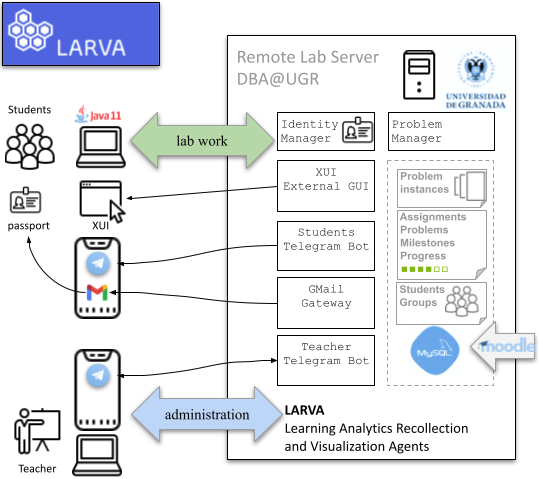
\includegraphics[width=0.60\textwidth]{estado/LARVA2122Architecturec.png}
    \caption{Arquitectura del Servidor Remoto. Por un lado, contiene el laboratorio virtual para sistemas multiagente distribuidos. Además, los alumnos también pueden consultar su progreso y el de sus compañeros a través de un Bot de Telegram. Por otro lado, el profesor también puede conocer el número de objetivos conseguidos por cada uno de sus grupos de alumnos.}
    \label{fig:architecture}
\end{figure}

Este servidor contiene varios mundos virtuales y se encarga de registrar y almacenar las interacciones con él \cite{Vidal_2016}. Cada mundo virtual es una matriz cuadrada que representa espacios abiertos (en color blanco), obstáculos (en negro) y objetivos (en rojo) tal y como se muestra en la Figura \ref{fig:map}. Los agentes de los alumnos deben entrar en uno de esos mundos virtuales, percibir su vecindario, navegar a través de los espacios abiertos (empleando alguna clase de heurística exploratoria), evitar obstáculos y tratar de llegar al objetivo. En total, cada uno de los problemas planteados requieren de cinco pasos (o \emph{milestones}) hasta su consecución.

\begin{figure}[H]
    \centering
    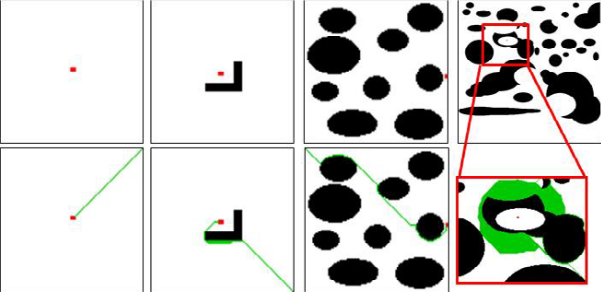
\includegraphics[width=0.60\textwidth]{estado/virtualworlds.png}
    \caption{Alguno de los mapas que el alumnado debe resolver. Los agentes de los grupos de estudiantes deben acceder a uno de esos mundos y deben alcanzar los objetivos (coloreados en rojo) navengado a través del mundo y evitando los obstáculos (coloreados en negro). Alguno de los mundos no son resolubles porque el objetivo no se puede alcanzar con el objetivo de forzar a los agentes de los alumnos a razonar acerca de la irresolubilidad. Las posibles trayectorias están marcadas en verde.}
    \label{fig:map}
\end{figure}

La percepción del agente de su entorno es crítica para resolver estos mundos. En este laboratorio virtual los alumnos pueden configurar cuál de los siguientes sensores estarán enchufados en sus agentes (cualquier combinación de ellos):

\begin{itemize}
	\item Un \textbf{GPS} que indica al agente sus coordenadas $(x,y)$ en el mundo virtual.
	\item Un \textbf{sensor de batería}. Cada agente está alimentado con una batería cuya capacidad es limitada y cuya carga decrece conforme el agente realiza algún movimiento. La batería nunca debe ser vaciada por completo.
	\item Un \textbf{sensor radar} que informa al agente acerca de los tipos de celdas que lo rodean con una percepción local de 5x5 (observar Figura \ref{fig:sensorb}).
	\item Un \textbf{sensor escáner} que actúa como \emph{detector del objetivo} e indica al agente la distancia al mismo medida desde cada una las celdas de su entorno 5x5 (observar Figura \ref{fig:sensorc}).
\end{itemize}

\begin{figure}[H]
\centering
\begin{subfloat}[] {
\centering
\begin{tikzpicture}[scale=0.8]
	\fill (0,0) rectangle ++ (1,1); 
    \fill (0,1) rectangle ++ (1,1);
    \fill (0,2) rectangle ++ (1,1);
    \fill (0,3) rectangle ++ (1,1);
    \fill (0,4) rectangle ++ (1,1); 
    \fill (1,4) rectangle ++ (1,1);
    \fill (2,4) rectangle ++ (1,1);
    \fill (3,4) rectangle ++ (1,1);
    \fill (4,4) rectangle ++ (1,1);
    \fill (4,3) rectangle ++ (1,1);
    \fill (4,2) rectangle ++ (1,1);
    \fill (3,2) rectangle ++ (1,1);
    \fill (2,1) rectangle ++ (1,1);
    \fill (3,1) rectangle ++ (1,1);
    \fill[red] (4,1) rectangle ++ (1,1);
 	\fill[green] (2,2) rectangle ++ (1,1); 
 	\draw[draw=gray] (0,0) grid (5,5);
\end{tikzpicture}
\label{fig:sensora}   
}
\end{subfloat}   
\hfill  
\begin{subfloat}[] {
\centering
\begin{tikzpicture}[scale=0.8]
\node at (0.5,0.5) {1};
\node at (0.5,1.5) {1};
\node at (0.5,2.5) {1};
\node at (0.5,3.5) {1};
\node at (0.5,4.5) {1};
\node at (1.5,0.5) {0};
\node at (1.5,1.5) {0};
\node at (1.5,2.5) {0};
\node at (1.5,3.5) {0};
\node at (1.5,4.5) {1};
\node at (2.5,0.5) {0};
\node at (2.5,1.5) {1};
\fill[green] (2,2) rectangle ++ (1,1);
\node at (2.5,2.5) {0};
\node at (2.5,3.5) {0};
\node at (2.5,4.5) {1};
\node at (3.5,0.5) {0};
\node at (3.5,1.5) {1};
\node at (3.5,2.5) {1};
\node at (3.5,3.5) {0};
\node at (3.5,4.5) {1};
\node at (4.5,0.5) {0};
\node at (4.5,1.5) {2};
\node at (4.5,2.5) {1};
\node at (4.5,3.5) {1};
\node at (4.5,4.5) {1};
\draw (0,0) grid (5,5);
\end{tikzpicture}
\label{fig:sensorb}   
}    
\end{subfloat}
\hfill
\begin{subfloat}[] {
\centering
\begin{tikzpicture}[scale=0.8]
\node at (0.5,0.5) {4};
\node at (0.5,1.5) {4};
\node at (0.5,2.5) {4};
\node at (0.5,3.5) {4};
\node at (0.5,4.5) {4};
\node at (1.5,0.5) {3};
\node at (1.5,1.5) {3};
\node at (1.5,2.5) {3};
\node at (1.5,3.5) {3};
\node at (1.5,4.5) {3};
\node at (2.5,0.5) {2};
\node at (2.5,1.5) {2};
\fill[green] (2,2) rectangle ++ (1,1);
\node at (2.5,2.5) {2};
\node at (2.5,3.5) {2};
\node at (2.5,4.5) {3};
\node at (3.5,0.5) {1};
\node at (3.5,1.5) {1};
\node at (3.5,2.5) {1};
\node at (3.5,3.5) {2};
\node at (3.5,4.5) {3};
\node at (4.5,0.5) {1};
\node at (4.5,1.5) {0};
\node at (4.5,2.5) {1};
\node at (4.5,3.5) {2};
\node at (4.5,4.5) {3};
\draw (0,0) grid (5,5);
\end{tikzpicture}
\label{fig:sensorc}
}       
\end{subfloat}
\caption{Un agente (representado por una celda verde en el centro de cada figura) tiene una percepción local de su entorno: solamente percibe el entorno 5x5 de celdas colindantes. El Radar \ref{fig:sensorb} muestra dicho entorno 5x5 que rodea al agente e informa de si una celda está vacía (valor $0$), de si hay un obstáculo (valor $1$) o de si hay un objetivo (valor $2$). El Escáner \ref{fig:sensorc} muestra la distancia de cada una de las celdas colindantes al objetivo.}
\label{fig:sensors}
\end{figure}

Basados en su percepción del mundo virtual, cada agente decidirá ejecutar alguna de las siguientes acciones en su entorno implementando cualquier heurística o proceso de búsqueda.

\begin{itemize}
	\item LOGIN. Entrar en cualquiera de los mundos virtuales.
	\item MOVE. Mover al agente a una de las $8$ celdas adyacentes y gastar una cierta cantidad de batería. Si la celda destino es un obstáculo o el agente se queda sin batería, el agente se rompe y sale del mundo  virtual.
	\item REFUEL. El agente recarga completamente su batería. A los agentes se les permite recargar su batería tantas veces como deseen.
\end{itemize}

\section{Funcionamiento del laboratorio virtual}\label{sec:funcionamiento}

Supongamos que una persona tiene que completar una determinada tarea con nueve pasos o milestones diferentes, numerados del $1$ al $9$, de los cuales los pasos $3$, $6$ y $9$ tienen una recompensa. Esta persona podría intentar pasar por cada una de las subtareas tantas veces como considere oportuno para conseguir todas las recompensas, llevando a cabo un registro de su actividad. Por ejemplo, la Figura \ref{fig:example} muestra uno de estos registros. Ignorando el paso 1, que sólo se utiliza para marcar el inicio del registro, esta persona ha realizado $35$ pasos, repitiendo el paso $2$ siete veces, el paso $3$ seis veces, el paso $4$ dos veces, el paso $5$ seis veces, el paso $6$ cinco veces, el paso $7$ cuatro veces, el paso $8$ cuatro veces y el paso $9$ sólo una vez. Este comportamiento puede representarse con un grafo dirigido ponderado (cíclico) donde los
nodos representan los pasos dados y las aristas se ponderan con la frecuencia detectada en el registro (Figura \ref{fig:example}), de modo que el número de veces que se ejecuta un paso viene dado por la suma de los pesos de sus aristas entrantes, lo cual denominaremos factor de grado de entrada (\emph{in-degree}) de aquí en adelante.

\begin{figure}[H]
    \centering
    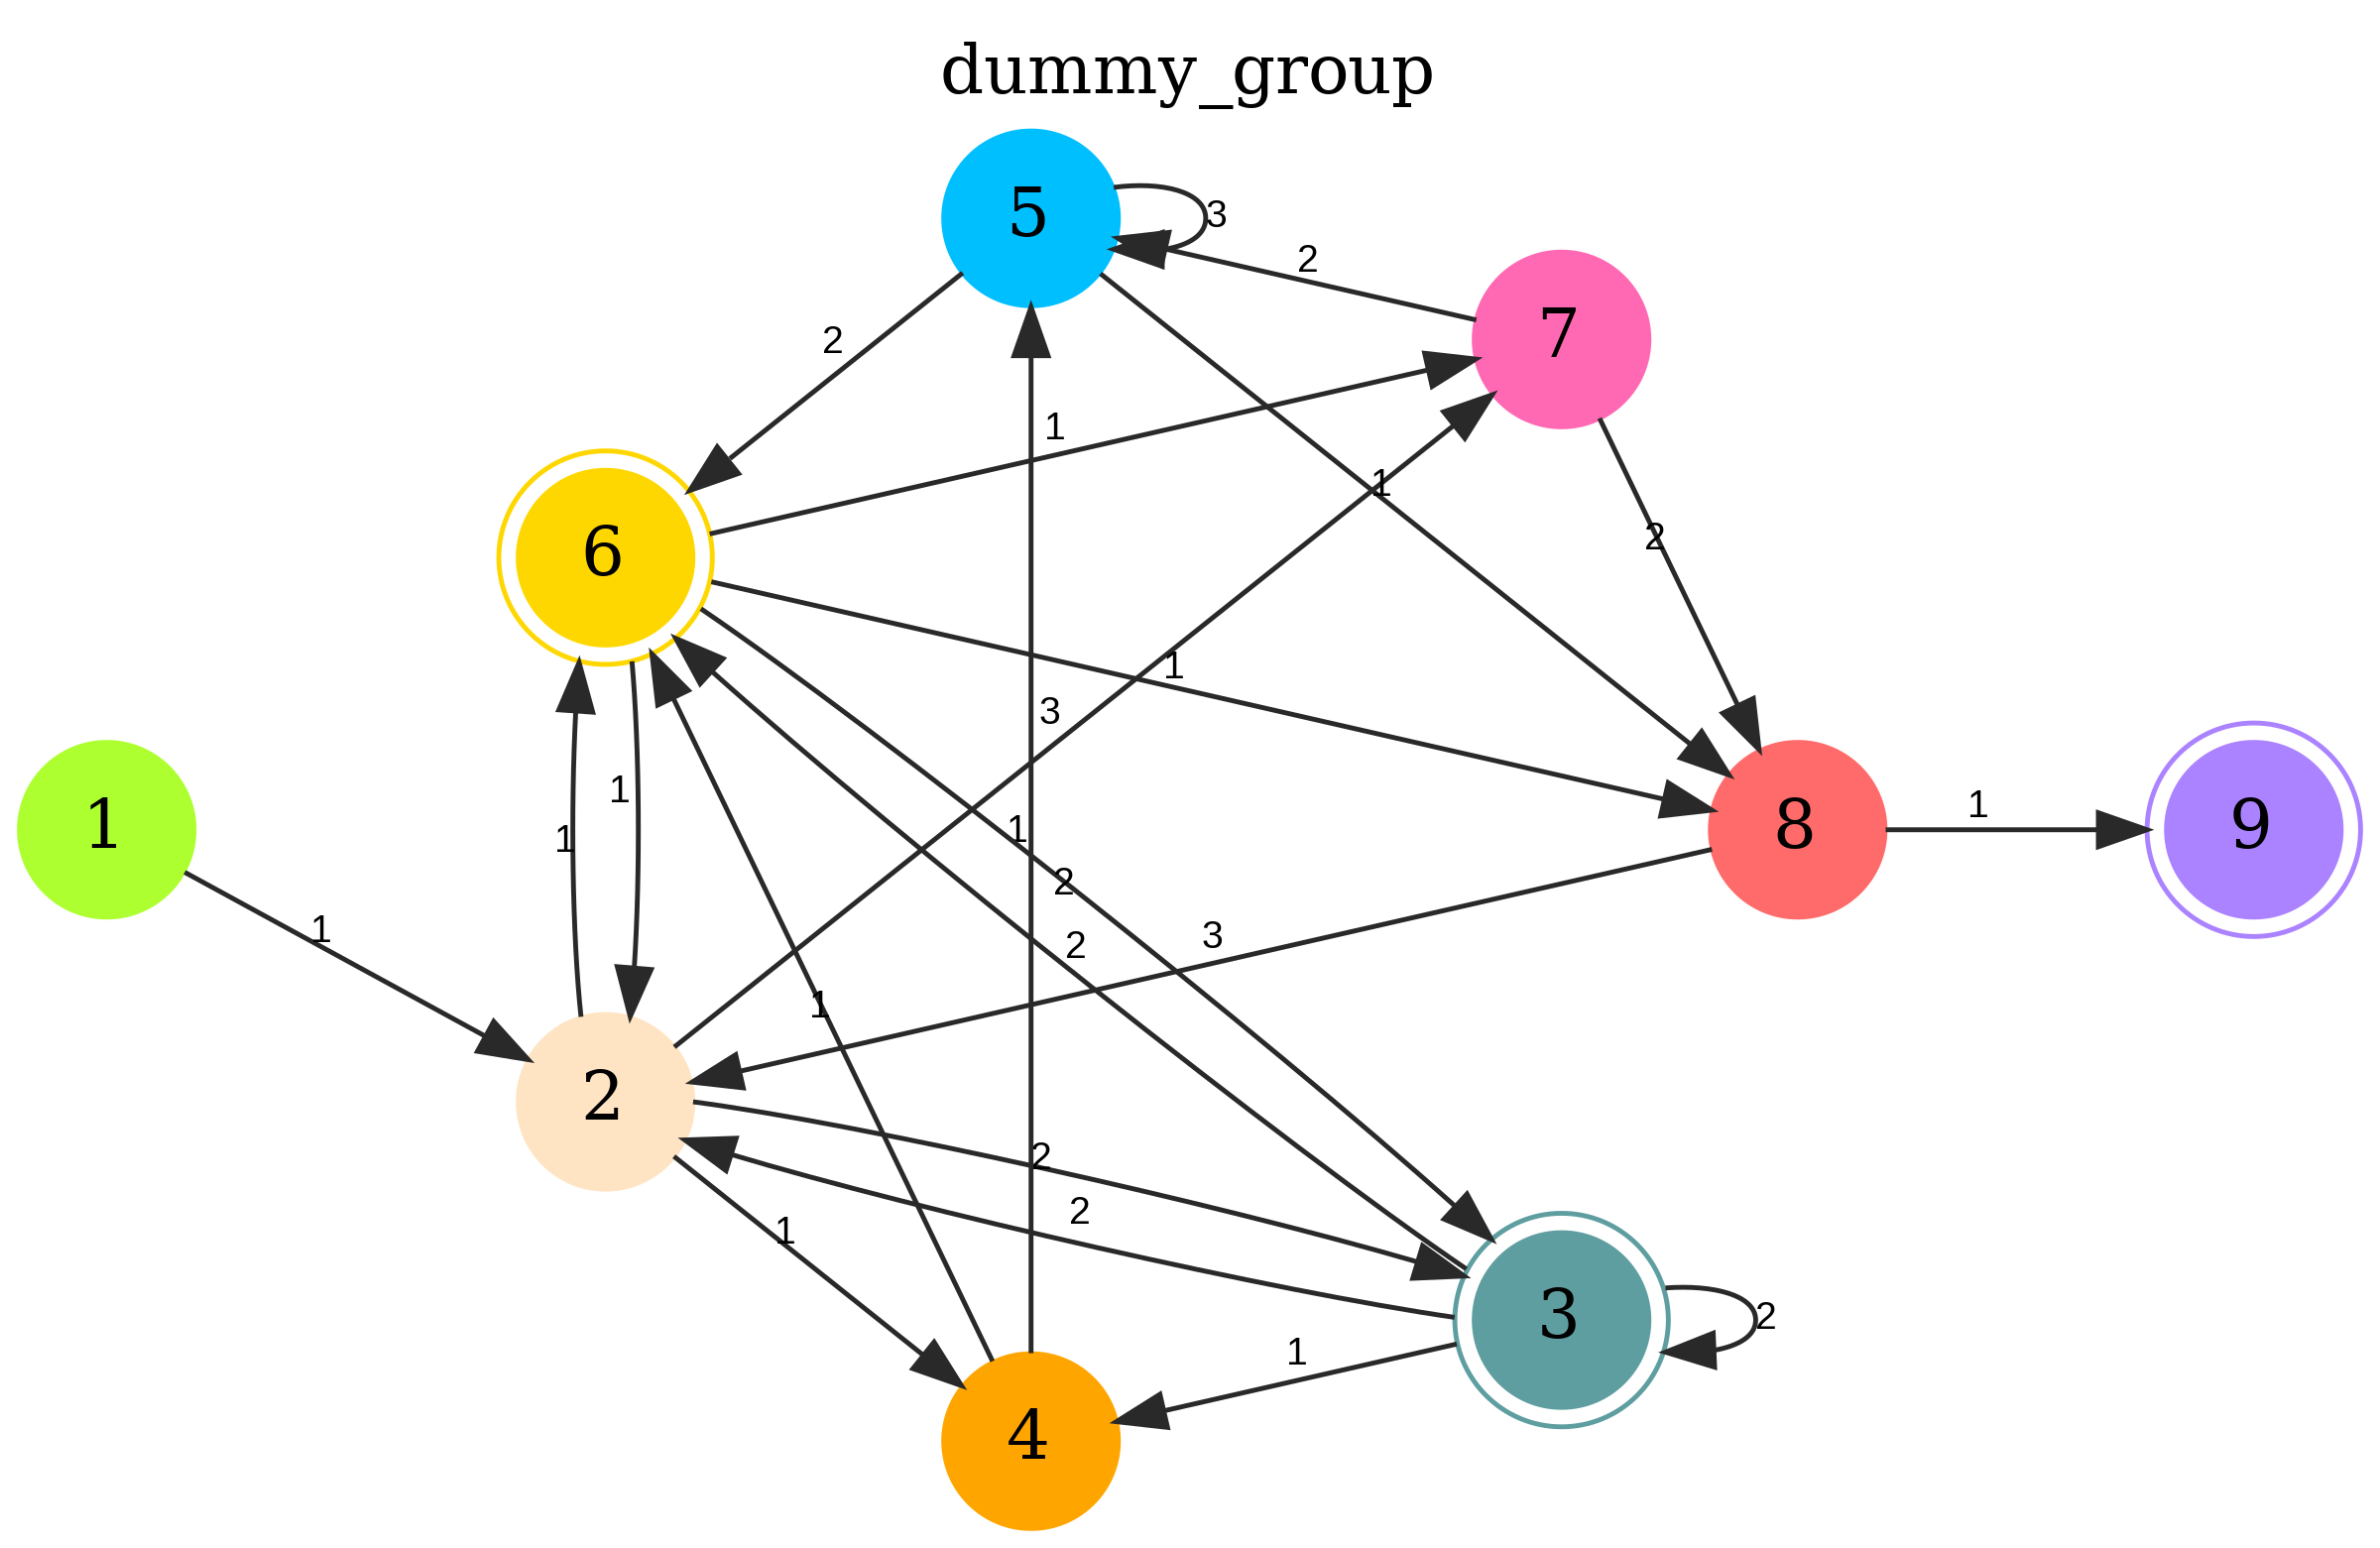
\includegraphics[width=0.60\textwidth]{estado/example.png}
    \caption{La secuencia correspondiente al grafo es: $1$ $2$ $(3)$ $2$ $4$ $5$ $5$ $(6)$ $(3)$ $(3)$ $4$ $(6)$ $7$ $5$ $5$ $5$ $8$ $2$ $(6)$ $(3)$ $2$ $7$ $5$ $(6)$ $8$ $2$ $(3)$ $(3)$ $(6)$ $2$ $7$ $8$ $2$ $7$ $8$ $(9)$. Así pues, el gráfico muestra el comportamiento básico de un determinado grupo en el que se repiten $9$ pasos, tres de los cuales, representados entre paréntesis, tienen una recompensa.}
    \label{fig:example}
\end{figure}

Este registro lineal de actividades refleja exactamente cómo se almacena la realización de tareas de laboratorio en LARVA \cite{Vidal_2022}, \cite{Vidal_2023}, un laboratorio virtual \cite{Vidal_2016} diseñado con un único propósito: permitir a los estudiantes alcanzar su mayor éxito. Para ello, LARVA mantiene un registro completo de la actividad de los alumnos, por lo que su evaluación se basa no sólo en los objetivos alcanzados, sino también en su progreso. Además, cuenta con un sistema de retroalimentación multimodal \cite{Vidal_2022} para mantener a los estudiantes informados sobre su progreso, en tiempo real, gracias a mensajes de chat de Telegram enviados directamente a sus teléfonos móviles. Puede demostrarse que cuanto antes reciban el feedback sobre su actividad y cuanto más rica sea esta retroalimentación, mayor será la autorregulación y la eficacia de la experiencia de aprendizaje \cite{Keller_1968}.

Revelar este comportamiento también puede ser útil para el profesor para detectar, cuanto antes, posibles dificultades de los alumnos para completar sus tareas y permitir una intervención clave por parte del profesor. Pero, ¿cómo detectar estas desviaciones del rendimiento esperado y con qué antelación podrían detectarse? Además, ¿sería posible ignorar cualquier detalle sobre los indicadores de progreso habituales asociados al rendimiento, como el momento de los éxitos y fracasos, la perseverancia, etc., para no depender demasiado en la ``eficiencia clásica'', y centrarse en las características topológicas del comportamiento de los alumnos? Para principiantes, en la Figura \ref{fig:extreme} se muestran dos comportamientos extremos. Por un lado, en la Figura \ref{fig:bad}, después de $372$ sesiones, la mayoría de ellas quemadas en los $3$-$4$ preliminares pasos, acaba con muy pocas sesiones en los últimos problemas, una especie de piloto automático, y resuelve $7$ de cada $9$ problemas. Por otro lado, en la Figura \ref{fig:good}, después de $297$ sesiones (¿podría considerarse como un menor esfuerzo?) muestra una exploración bastante exhaustiva de las alternativas y termina con 9 de 9 problemas resueltos. Este
documento responde con éxito a todas estas preguntas a partir de un sólido análisis basado en evidencias de los registros de los últimos siete años de este laboratorio virtual. Las siguientes secciones están dedicadas a discutir trabajos similares en la literatura, a presentar el escenario y la hipótesis principal y, a continuación, a extraer las principales conclusiones tras un análisis exhaustivo de los datos registrados. Todos los conjuntos de datos mencionados en este documento y todos los artefactos de software, completamente escritos en R, están abiertos y disponibles en GitHub \footnote{\href{https://github.com/maribel00/Analysis-of-processes}{https://github.com/maribel00/Analysis-of-processes}}.

\begin{figure}[H]
\centering
\subfloat[Grafo acíclico dirigido que captura el comportamiento de un grupo con $372$ sesiones de trabajo.]{\label{fig:bad}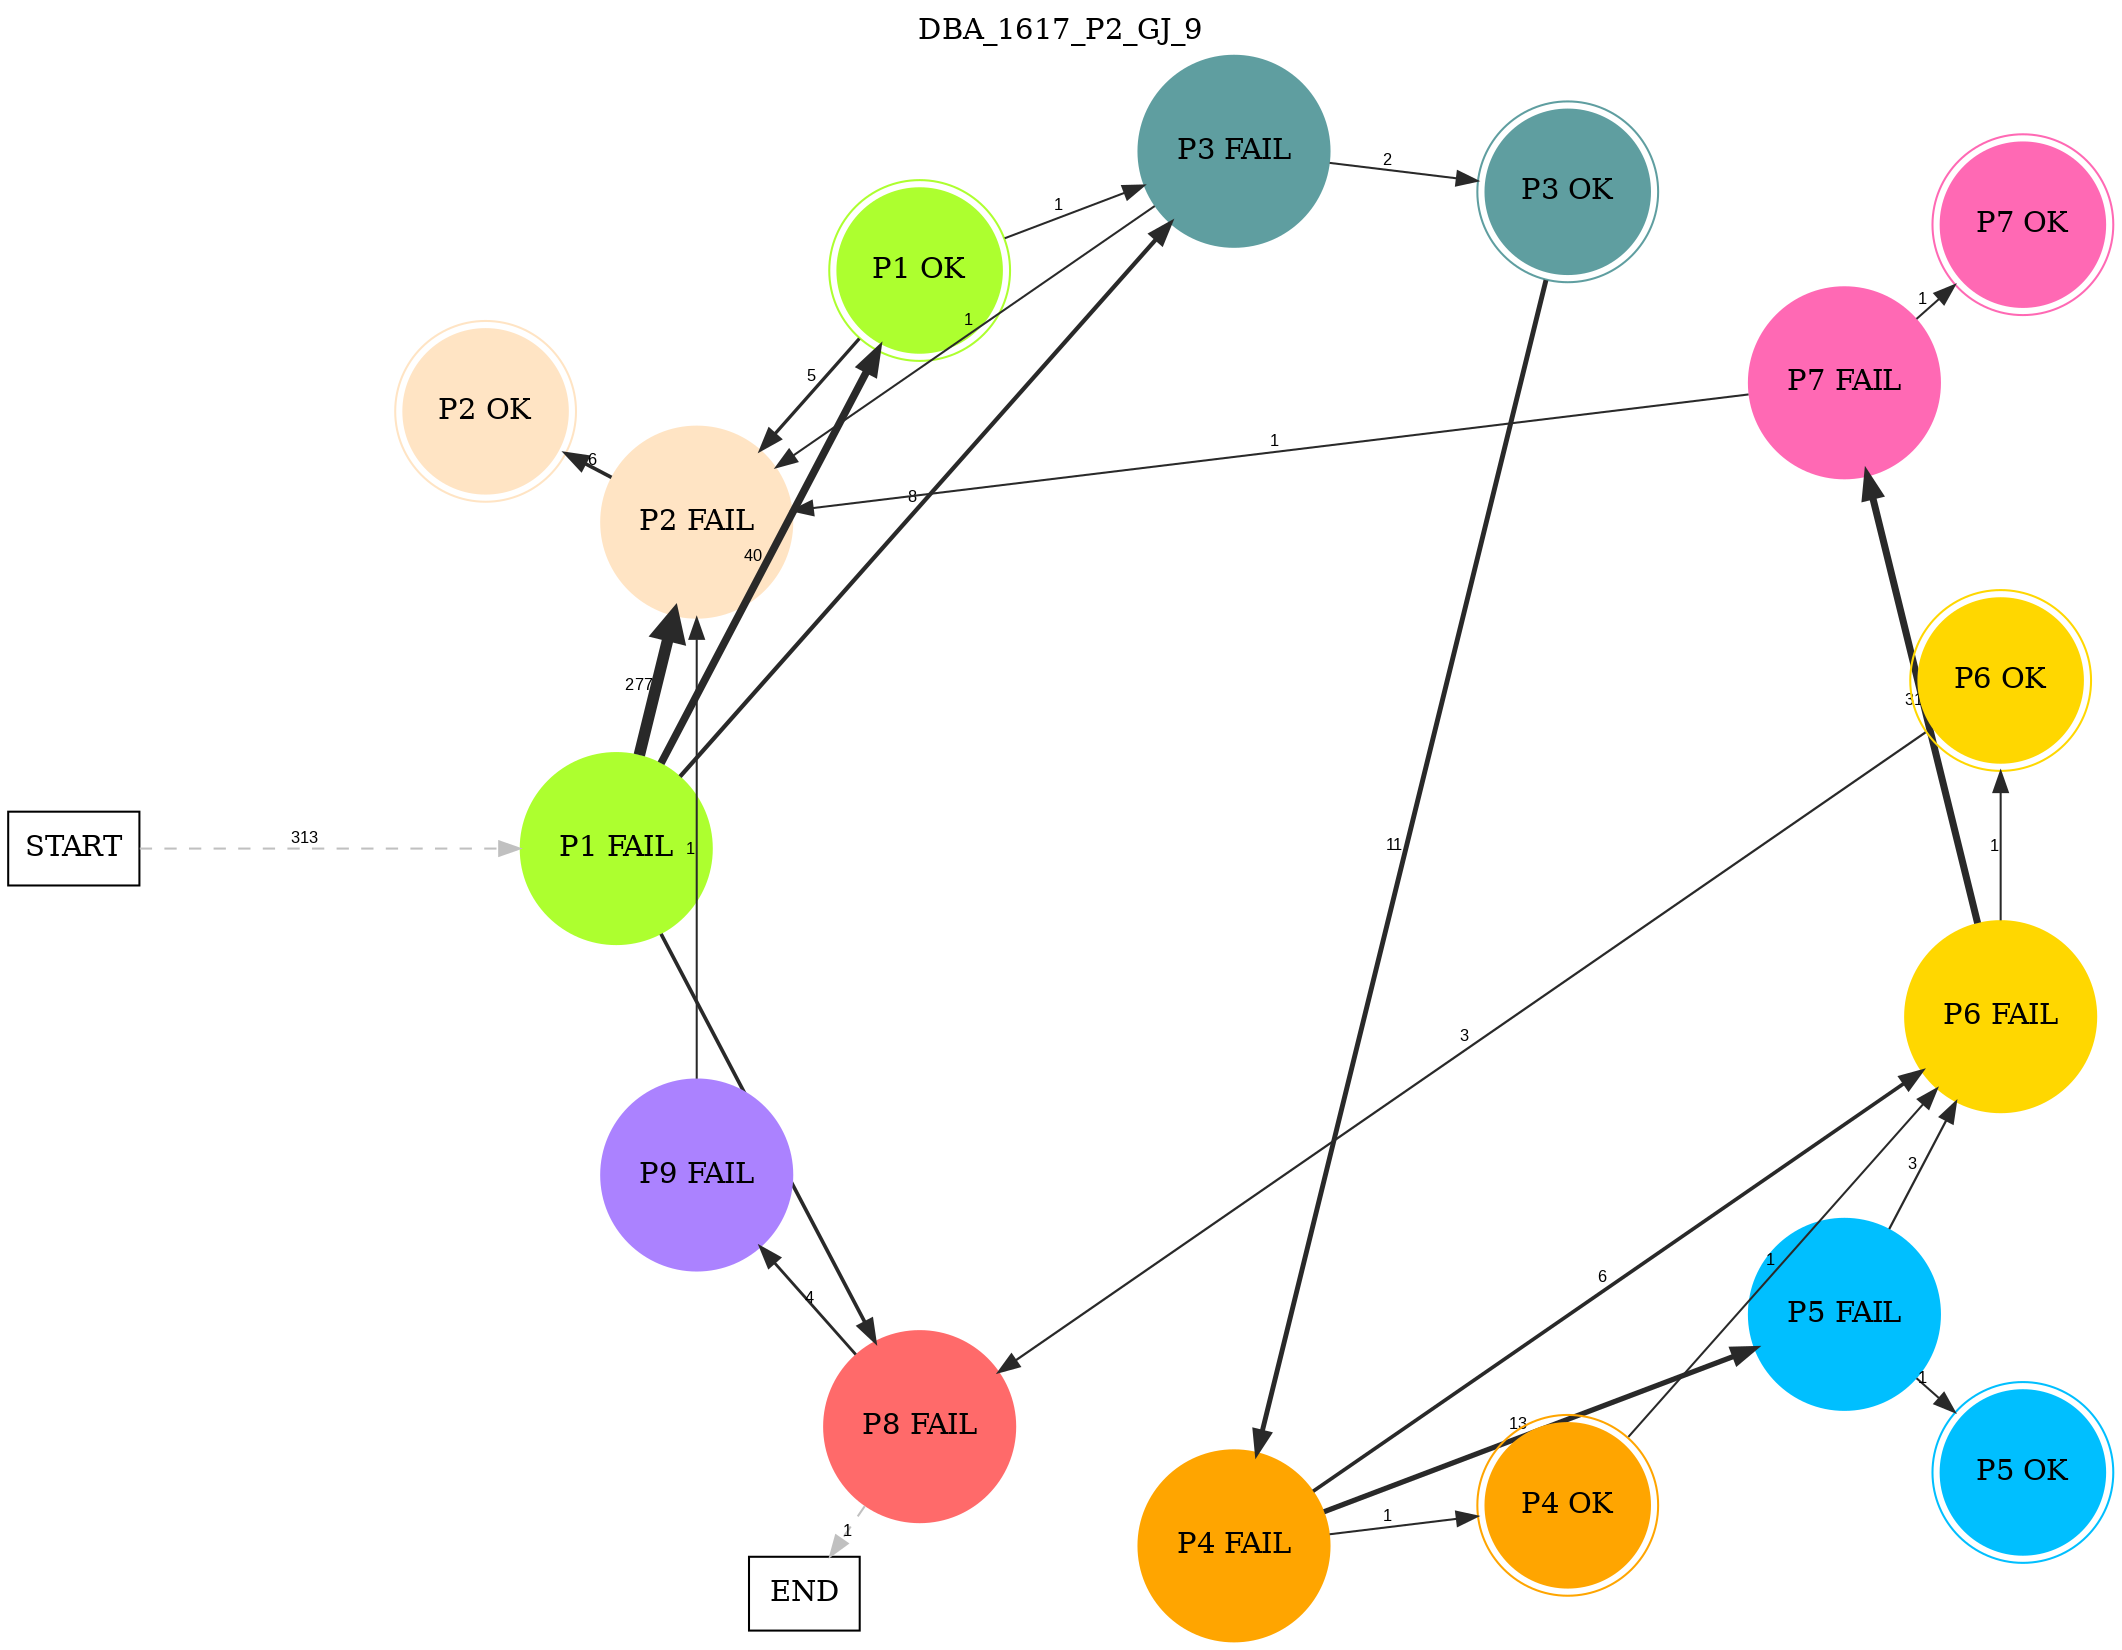
\includegraphics[width=0.47\textwidth]{estado/DBA_1617_P2_GJ_9.png}}\qquad
\subfloat[Grafo acíclico dirigido que captura el comportamiento de un grupo con $297$ sesiones de trabajo.]{\label{fig:good}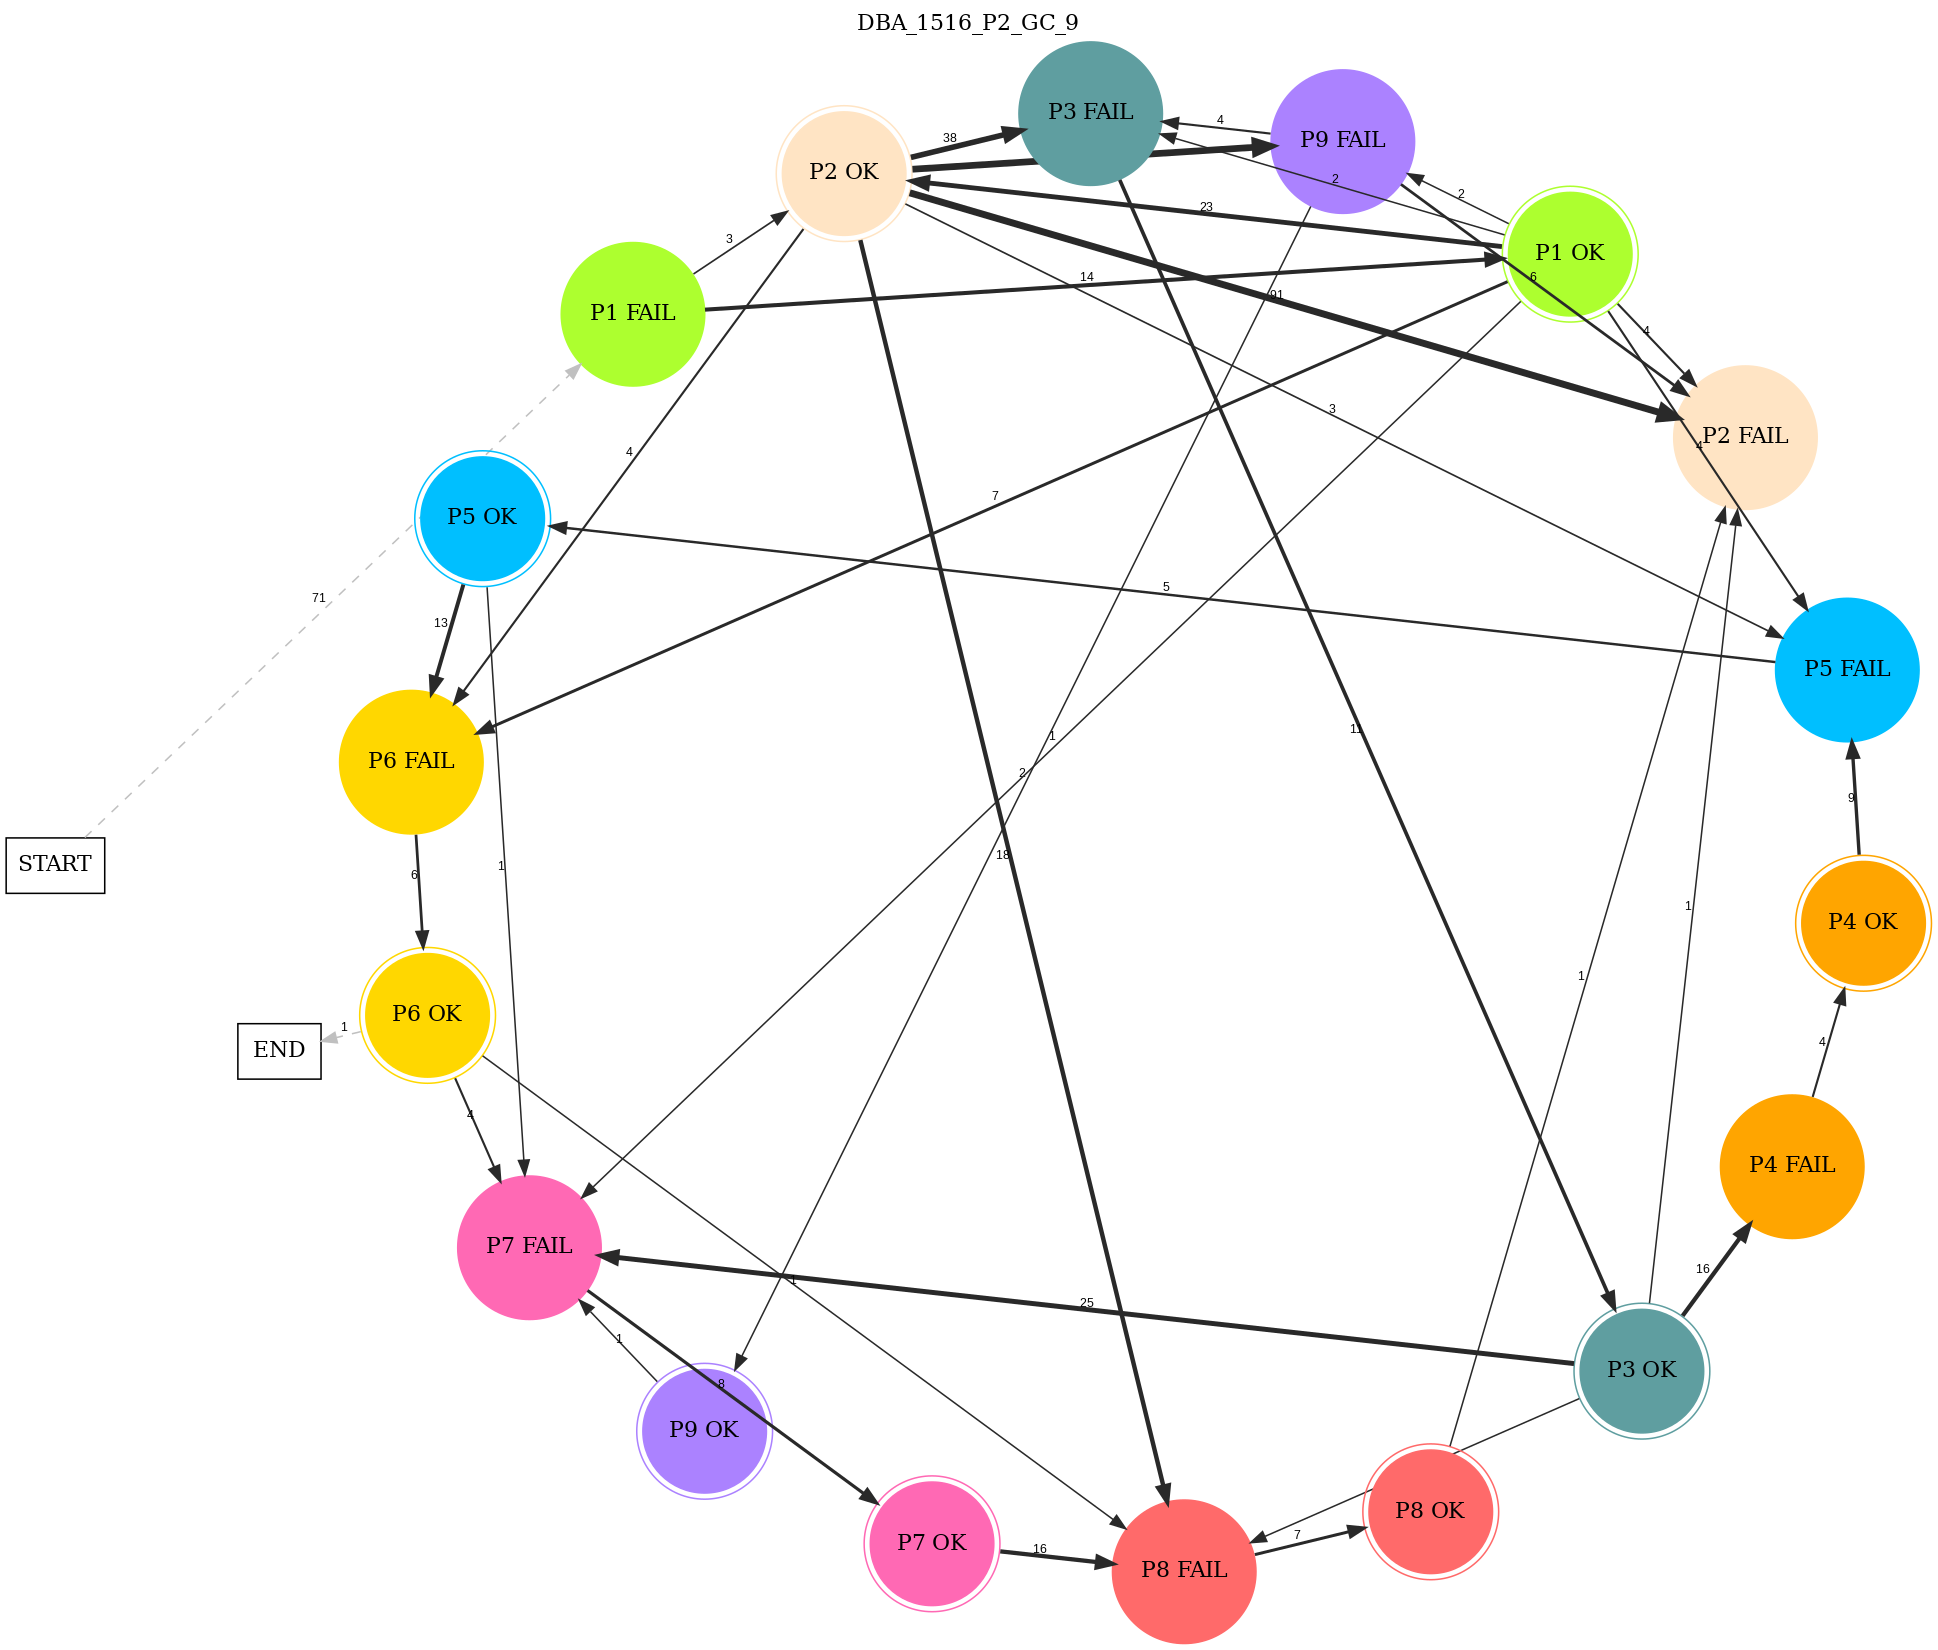
\includegraphics[width=0.47\textwidth]{estado/DBA_1516_P2_GC_9.png}}
\caption{Dos comportamientos reales diferentes de grupos enfrentándose a las mismas tareas de laboratorio.}
\label{fig:extreme}
\end{figure}

\section{Descripción del escenario inicial}\label{sec:initial}

Como se ha mencionado anteriormente, este estudio se ha llevado a cabo a partir de los datos de una asignatura obligataria de 4º curso de la rama Ingeniería del Software en la Universidad de Granada registrados a través de un laboratorio virtual \cite{Vidal_2016}. Esta asignatura sigue la estructura típica del Sistema Personalizado de Instrucción \cite{Keller_1968} donde el progreso de los estudiantes se monitorea continuamente gracias a un sistema de hitos y logros continuos, proporcionando tanta retroalimentación como sea posible y tan pronto como sea posible. Así, durante el curso, los alumnos se organizan en grupos (de $4$-$5$ miembros cada uno) y cada grupo debe resolver una serie de tareas o problemas. De ahora en adelante denotaremos al conjunto de problemas por $P = \left\lbrace p_i \right\rbrace$ y al número de problemas a resolver por $n = |P|$.

Por lo general, el número de problemas es $n = 9$ y podrían considerarse como un conjunto de misiones a realizar en escenarios similares. Adicionalmente, cada problema ha sido cuidadosamente elaborado por el profesor para que requiera un nivel de dificultad creciente por parte de los estudiantes de tal forma que la estrategia para resolver $p_i$ puede no ser lo suficientemente buena resolver $p_{i+1}$ pero la estrategia para resolver $p_{i+1}$ también debe ser válida en $p_i$. Estos problemas están abiertos durante un determinado periodo de tiempo durante el cual los estudiantes pueden abrir los problemas tantas veces como necesiten, ya sea para intentar resolver el problema, para mejorar sus soluciones en estos problemas o para probar nuevas estrategias. Además de esto, cada problema $p_i$ se ha diseñado como una secuencia de $5$ hitos consecutivos, también en nivel creciente de dificultad:

\begin{equation}
p_i = \left\lbrace p_i^1 , p_i^2 , p_i^3 , p_i^4 , p_i^5 \right\rbrace
\end{equation}

siendo $p_i^1$ el suceso de sólo abrir el problema $i$ y $p_i^5$ la obtención de una solución válida para $p_i$. Estos hitos deben ser alcanzados progresivamente por los alumnos, por lo que todo acaba por empujando a los alumnos un poco hacia adelante en sus capacidades \cite{Keller_1968}. Por lo tanto, a medida que los estudiantes progresan en el laboratorio, dejan un registro de sus logros, que se llamará \emph{comportamiento}, $B^g$, de un determinado grupo $g$, y está compuesto por una secuencia de sesiones.

\begin{equation}
B^g = \left\lbrace ^sp_i^k,\dots \right\rbrace
\end{equation}

Cada \emph{sesión} del laboratorio virtual $^sp_i^k$ se etiqueta como el mayor hito $k$ alcanzado en cada problema $p_i$ y un número natural secuencial $s$ que es un registro del tiempo actual del sistema. Además, se utiliza una marca $A$ para señalar el inicio del de laboratorio y un indicador $Z$ para señalar el cierre del mismo.

\begin{equation}
B^g = \left\lbrace ^0A \right\rbrace \cup \left\lbrace ^sp_i^k,\dots \right\rbrace \cup \left\lbrace Z \right\rbrace
\end{equation}

\begin{table}[H]
\centering
\caption{El comportamiento de un grupo ficticio con $20$ sesiones de trabajo en el laboratorio virtual.}
\label{tab:sequence}
\begin{tabular}{cccccccccccc}
$^0A$ & $^1p_1^1$ & $^2p_1^3$ & $^3p_1^5$ & $^4p_1^5$ & $^5p_1^5$ & $^6p_1^4$ & $^7p_2^3$ & $^8p_2^4$ & $^9p_1^5$ & $^{10}p_1^5$ \\ \hline
$^{11}p_2^5$  & $^{12}p_1^1$ & $^{13}p_2^5$ & $^{14}p_3^2$ & $^{15}p_3^4$ & $^{16}p_1^2$ & $^{17}p_3^3$ & $^{18}p_2^3$ & $^{19}p_3^4$ & $^{20}p_3^5$ & $Z$
\end{tabular}
\end{table}

Por ejemplo, en un escenario con tres problemas, la secuencia mostrada en la Tabla \ref{tab:sequence} podría ser un comportamiento factible $B$, que ya se introdujo en la Sección \ref{sec:funcionamiento}, y ahora se explica bajo una nueva perspectiva:

\emph{``Los estudiantes se han conectado $20$ veces al laboratorio virtual. En la primera sesión se abre el problema $p_1$ sin más éxito y en la segunda sesión se deja el problema $p_1$ a medias. No obstante, en la tercera sesión se resuelve completamente $p_1$ . Los estudiantes ponen en práctica nuevas estrategias y resuelven $p_1$ dos veces más. A continuación, introducen un nuevo cambio que casi resuelve $p_1$, acaba fallando y deja $p_2$ justo en la mitad. Después, tras algunos cambios, resuelven de nuevo $p_1$ en la sesión $9$ y $p_2$ en la sesión $11$. Después, cambiaron algo en la implementación que resultó ser un fracaso en $p_1$ y acaban teniendo éxito en $p_3$ justo al final''.}

La Figura \ref{fig:groupsperyear} y Tablas \ref{tab:days} y \ref{tab:records} muestran información descriptiva de los datos registrados cada año sobre el comportamiento de $77$ grupos (en total casi $400$ alumnos). Como se puede ver, hay registros de $7$ años consecutivos y un total de $30672$ sesiones de trabajo en el laboratorio virtual. A continuación, el reto es cómo extraer un gráfico como los que se muestran en la Sección \ref{sec:funcionamiento} y cómo utilizarlos para detectar, lo antes posible, los grupos con dificultades para progresar.
\chapter{Introducción a la Minería de Procesos y trabajos previos}\label{sec:chapterII}
\addcontentsline{toc}{chapter}{Introducción a la Minería de Procesos y trabajos previos}

Las transacciones de los agentes en estos mundos virtuales registradas en el servidor no sólo son importantes desde el punto de vista de la evaluación del alumnado, sino que también nos proporcionan información de cómo se han resuelto los problemas propuesto, hito por hito, y son un reflejo de la estrategia seguida por cada uno de los equipos para intentar resolver todos los mundos.

Para tratar de desvelar estas estrategias ocultas se usarán técnicas de minería de procesos, considerando una estrategia como el proceso seguido por los estudiantes hasta llegar al objetivo. La minería de procesos puede definirse como la disciplina que tiene como objetivo descubrir, monitorear y mejorar procesos de negocio mediante el análisis de las transacciones del proceso que se han almacenado en algún sistema de información \citep{Mayorga_2015}. Así pues, la minería de procesos para la educación es como los rayos X para la medicina: hacen visible lo invisible, en aras de un conocimiento mucho más preciso de la situación y de la planificación de nuevas intervenciones. Pero, ¿hasta qué punto es pertinente atenerse a un gráfico extraído de registros de eventos en lugar de, por ejemplo, una representación tabular equivalente? Este estudio se concibió bajo esta perspectiva y analiza el comportamiento de los alumnos no como en la forma clásica de producir restricciones temporales, de rendimiento o de cualquier semántica asociada a su rendimiento o a sus notas. Por el contrario, este trabajo analiza justo la topología pura y desnuda del comportamiento y proporciona pruebas sólidas de que estas topologías están, cómo no, también correlacionadas con el rendimiento, en particular, para la detección de grupos de estudiantes de perfil bajo.

Actualmente, con el desarrollo y el creciente interés de las plataformas educativas y de toda la tecnología relacionada con las mismas, los sistemas de información nos permiten recoger todo tipo de información. Esto puede incluir desde información de bajo nivel (clicks del ratón) hasta información de alto nivel (realización de una actividad en particular dentro de la plataforma). Es decir, estos sistemas tienen la capacidad de almacenar datos temporales de diversa índole, como cadenas de clicks, registros de chats, históricos de modificación de documentos, registros de uso de los diferentes recursos educativos, etc. \cite{bogarin2018survey}. La minería de procesos puede usar todos estos logs para descubrir, monitorear y mejorar los procesos educativos. Surge así la denominada minería de procesos educacional (en inglés, \emph{educational process mining}). No obstante, cabe destacar que, aunque en este trabajo fin de grado nos centraremos en la minería de procesos en el ámbito educativo, ésta también tiene numerosas aplicaciones en el área sanitaria, en el ámbito empresarial, institucional etc.

Como se ha mencionado anteriormente, el uso de técnicas de Minería de Procesos está suscitando un enorme interés y hay cantidades ingentes de artículos y trabajos relacionados que podrían referenciarse, especialmente cuando los profesores crean laboratorios virtuales \cite{Elmoazen_2023} o servicios \emph{online} como Coursera \cite{mukala2015learning}. También hay algunas revisiones excelentes de la Minería de Proceesos en el contexto educativo como \cite{dos2019process}, donde se recalca que la educación es la cuarta área más importante en la que se están aplicando técnicas de Minería de Procesos para detectar estilos de aprendizaje (o, en inglés, \emph{learning styles}), o incluso mejor, en \cite{bogarin2018survey} donde los autores también ponen el énfasis en el análisis de grafos como estructura subyacente del comportamiento (concepto de \emph{graph mining}). Además, en dicho artículo se presentará lo que se denomina \emph{intention mining} que hace referencia a la minería de procesos aplicada con el objetivo de anticipar el comportamiento. Los mismos autores en \cite{bogarin2018discovering} también apuntan a una cuestión muy interesante e íntimamente relacionada con este trabajo: cómo utilizar técnicas de Minería de Procesos para detectar a los que más necesitan la ayuda del profesor, simplemente observando el patrón de interacción de los alumnos con el \emph{LMS} (\emph{Learning Management System}). Esta relación del alumno con los recursos disponibles, normalmente en línea, también se explora en \cite{mukala2015learning}, en el que el uso de la Minería de Procesos no es realmente descubrimiento, sino el cumplimiento, para detectar si los alumnos se comportan como se espera de ellos o en la forma en que utilizan los recursos disponibles \cite{juhavnak2019using}. En \cite{sedrakyan2016process} los autores analizan el potencial del
feedback que el PM (\emph{Process Mining}) puede dar a los alumnos, muy en la línea de \citep{Keller_1968} para fomentar la autorregulación de los alumnos. En todos ellos las principales métricas utilizadas para orientar el estudio son las ``clásicas'' relacionadas con los recursos, las personas o el material de aprendizaje a través de un enfoque cuantitativo para puntuar el comportamiento de los estudiantes. Este trabajo fin de grado adoptará un enfoque diferente e intenta analizar puramente la topología del grafo dirigido que describe el comportamiento de un determinado grupo de prácticas.

\begin{figure}[H]
    \centering
    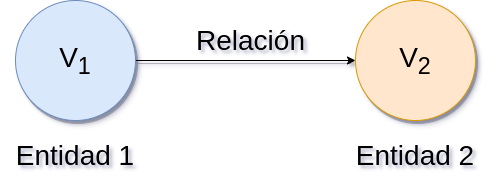
\includegraphics[width=0.40\textwidth]{previo/diagrama.png}
    \caption{Los nodos de los grafos pueden representar recursos o herramientas, personas o instituciones e incluso unidades temáticas. Asimismo, las relaciones entre nodos también llevan asociadas un significado (energía o frecuencia, proximidad o distancia entre ambos o predecedencia u orden entre ambos).}
    \label{fig:classification}
\end{figure}

Los trabajos anteriormente citados así como los que se realizarán en este trabajo fin de grado relacionados con la Minería de Procesos son susceptibles a ser clasificados. Así pues, dado un grafo $G = (V,E)$ donde $V$ y $E$ son sus respectivos conjuntos de vértices y aristas (Definición \ref{def:grafo}) siendo una parte del mismo la que se muestra en la Figura \ref{fig:classification}, se puede realizar una segmentación de los proyectos de minería de procesos atendiendo a qué representan sus nodos, qué significado tiene la relación entre éstos y el momento temporal al que nos estemos refiriendo. Así pues, atendiendo a todas estas características se ha realizado la clasificación de las técnicas de Minería de Procesos en el ámbito educativo que se muestra en el Cuadro \ref{tab:classification}.

\begin{table}[H]
\centering
\caption{Clasificación de las técnicas de Minería de Procesos aplicadas a la educación. Como podemos ver, pueden estar orientadas al pasado, al presente y al futuro.}
\label{tab:classification}
\begin{tabular}{|>{\centering\arraybackslash}m{2.5cm}|>{\centering\arraybackslash}m{4cm}|>{\centering\arraybackslash}m{4cm}|>{\centering\arraybackslash}m{4cm}|}
\hline
\rowcolor{orange!20}
\backslashbox{\footnotesize{\textbf{Nodos}}}{\footnotesize{\textbf{Aristas}}} & \footnotesize{\textbf{Energía} (Conteo)} & \footnotesize{\textbf{Cercanía} (Clustering)} & \footnotesize{\textbf{Orden} (Precedencia)} \\ 
\hline 
\cellcolor{orange!20}\footnotesize{Recursos (vídeos, texto) y \textbf{Herramientas}} &

\begin{tabular}[t]{
    | >{\scriptsize\centering\arraybackslash}m{1cm}
    | >{\scriptsize\centering\arraybackslash}m{2cm}|
  }
  \hline
  \cellcolor{cyan!25}\textbf{Pasado} & Coursera. Validación del curso. Uso de recursos (como podían ser los vídeos). \\
  \hline
  \cellcolor{lime!25}\textbf{Presente} & Patrones de uso. Seguimiento. Capacidad. \\
  \hline
  \cellcolor{pink!50}\textbf{Futuro} & Cuellos de botella (predicción de las necesidades del hardware). Posibles problemas. Recomendaciones. \\
  \hline
  \end{tabular}
  
  &

\begin{tabular}[t]{
    | >{\scriptsize\centering\arraybackslash}m{1cm}
    | >{\scriptsize\centering\arraybackslash}m{2cm}|
  }
  \hline
  \cellcolor{cyan!25}\textbf{Pasado} &  \\
  \hline
  \cellcolor{lime!25}\textbf{Presente} &  \\
  \hline
  \cellcolor{pink!50}\textbf{Futuro} &  \\
  \hline
  \end{tabular}
  
   &

\begin{tabular}[t]{
    | >{\scriptsize\centering\arraybackslash}m{1cm}
    | >{\scriptsize\centering\arraybackslash}m{2cm}|
  }
  \hline
  \cellcolor{cyan!25}\textbf{Pasado} &  \\
  \hline
  \cellcolor{lime!25}\textbf{Presente} &  \\
  \hline
  \cellcolor{pink!50}\textbf{Futuro} &  \\
  \hline
  \end{tabular}  
  
    \\ 
\hline 
\cellcolor{orange!20}\footnotesize{\textbf{Personas} e \textbf{Instituciones}} &

\begin{tabular}[t]{
    | >{\scriptsize\centering\arraybackslash}m{1cm}
    | >{\scriptsize\centering\arraybackslash}m{2cm}|
  }
  \hline
  \cellcolor{cyan!25}\textbf{Pasado} & Trabajo en grupo bien estructurado. Análisis de los alumnos con mejor/peor rendimiento. \\
  \hline
  \cellcolor{lime!25}\textbf{Presente} & Medidas intragrupos e intergrupos. Redes sociales. Evaluación de los alumnos. \\
  \hline
  \cellcolor{pink!50}\textbf{Futuro} & Liderazgo. Dominancia. Personas influyentes. Predicciones del rendimiento de los alumnos. \\
  \hline
  \end{tabular}

&

\begin{tabular}[t]{
    | >{\scriptsize\centering\arraybackslash}m{1cm}
    | >{\scriptsize\centering\arraybackslash}m{2cm}|
  }
  \hline
  \cellcolor{cyan!25}\textbf{Pasado} & Trabajo en equipo. \\
  \hline
  \cellcolor{lime!25}\textbf{Presente} &  \\
  \hline
  \cellcolor{pink!50}\textbf{Futuro} & Redes sociales: personas influyentes y colaboradores. \\
  \hline
  \end{tabular}  

& 

\begin{tabular}[t]{
    | >{\scriptsize\centering\arraybackslash}m{1cm}
    | >{\scriptsize\centering\arraybackslash}m{2cm}|
  }
  \hline
  \cellcolor{cyan!25}\textbf{Pasado} &  \\
  \hline
  \cellcolor{lime!25}\textbf{Presente} &  \\
  \hline
  \cellcolor{pink!50}\textbf{Futuro} &  \\
  \hline
  \end{tabular}  

\\ 
\hline 
\cellcolor{orange!20}\footnotesize{\textbf{Temáticas} (unidades temáticas de un curso), \textbf{Productos} o \textbf{bienes}} & 

\begin{tabular}[t]{
    | >{\scriptsize\centering\arraybackslash}m{1cm}
    | >{\scriptsize\centering\arraybackslash}m{2cm}|
  }
  \hline
  \cellcolor{cyan!25}\textbf{Pasado} & Validación del curso. Concienciación del profesorado. \\
  \hline
  \cellcolor{lime!25}\textbf{Presente} & Relaciones intergrupos. Redes sociales. \\
  \hline
  \cellcolor{pink!50}\textbf{Futuro} &  \\
  \hline
  \end{tabular} 

& 

\begin{tabular}[t]{
    | >{\scriptsize\centering\arraybackslash}m{1cm}
    | >{\scriptsize\centering\arraybackslash}m{2cm}|
  }
  \hline
  \cellcolor{cyan!25}\textbf{Pasado} &  \\
  \hline
  \cellcolor{lime!25}\textbf{Presente} &  \\
  \hline
  \cellcolor{pink!50}\textbf{Futuro} &  \\
  \hline
  \end{tabular} 

& 

\begin{tabular}[t]{
    | >{\scriptsize\centering\arraybackslash}m{1cm}
    | >{\scriptsize\centering\arraybackslash}m{2cm}|
  }
  \hline
  \cellcolor{cyan!25}\textbf{Pasado} & Similaridad del coseno. \\
  \hline
  \cellcolor{lime!25}\textbf{Presente} &  \\
  \hline
  \cellcolor{pink!50}\textbf{Futuro} & Planificación del curso. \\
  \hline
  \end{tabular}

\\
\hline 
\end{tabular} 
\end{table}
\chapter{Minería de Procesos}\label{sec:chapterIII}
\addcontentsline{toc}{chapter}{Minería de Procesos}

Como se ha comentado antes, cualquier posible evaluación de los alumnos basada meramente en los objetivos alcanzados es sólo una visión estática, sin muchas pistas sobre la dinámica que les ha llevado hasta ese punto. No sabemos muy bien cómo han llegado los alumnos hasta ahí y esta información es la clave para identificar a los grupos con dificultades que podrían necesitar la ayuda del profesor. Por lo tanto, vamos a emplear técnicas de Minería de Procesos \cite{aalst2016} para extraer las diferentes secuencias de eventos correlacionados del conjunto de datos original.

\section{Extracción de los procesos con DISCO}

Para la extracción de los procesos ocultos se empleará la muy conocida suite de minería de procesos Disco \cite{gunther2012disco}. Disco es una herramienta que permite crear mapas visuales a partir de los registros en cuestión de minutos.

\emph{Fuzzy Miner} \cite{gunther2007fuzzy} es un algoritmo de minería de procesos muy flexible y sólido que está detrás de Disco. En un proceso típico minado con Disco, cada actividad del proceso se etiqueta como en la Tabla \ref{tab:sequence} e incluye las frecuencias tanto de las actividades como de las transiciones entre actividades. Por lo tanto, la frecuencia de cada actividad representa el número de veces que esta actividad aparece en $B^g$. Por otro lado, la frecuencia de cada transición entre las actividades $x$ e $y$ representa el número de veces que la actividad $x$ aparece inmediatamente antes de la actividad $y$ en $B^g$.

Para crear los diagramas de Disco, se extraerán los campos de información más importantes del dataset:
\begin{enumerate}
\item El \emph{identificador del caso}, extraído de una clave aleatoria generada al principio de cada operación \texttt{LOGIN} y que distingue de manera unívoca cada sesión de trabajo de los estudiantes.
\item El \emph{agente}, que se refiere al nombre del grupo de estudiantes.
\item La \emph{fecha} y \emph{hora} a la que se registró la transacción.
\item El campo \emph{actividad} (\texttt{Activity}), que refleja la acción de los alumnos en el mundo virtual.
\item Varios campos de tipo \emph{recurso} (\texttt{Resource}) que proporcionan información adicional que puede sernos de utilidad a la hora de filtrar los registros.
\end{enumerate}

Así pues, se importarán el dataset de dos maneras diferentes, con el objetivo de estudiar tanto la frecuencia con que cada problema o mapa ha sido visitado como las acciones compuestas mapa-porcentaje superado. En la primera importación la \texttt{Activity} es el problema y el identificador del caso es el grupo. En la segunda importancia, por el contrario, la \texttt{Activity} es la composición del problema y el milestone y el identificador del caso son las sesiones. Las Figuras \ref{fig:problems} y \ref{fig:compound} muestran los diagramas obtenidos en cada uno de los casos.

\begin{figure}[H]
    \centering
    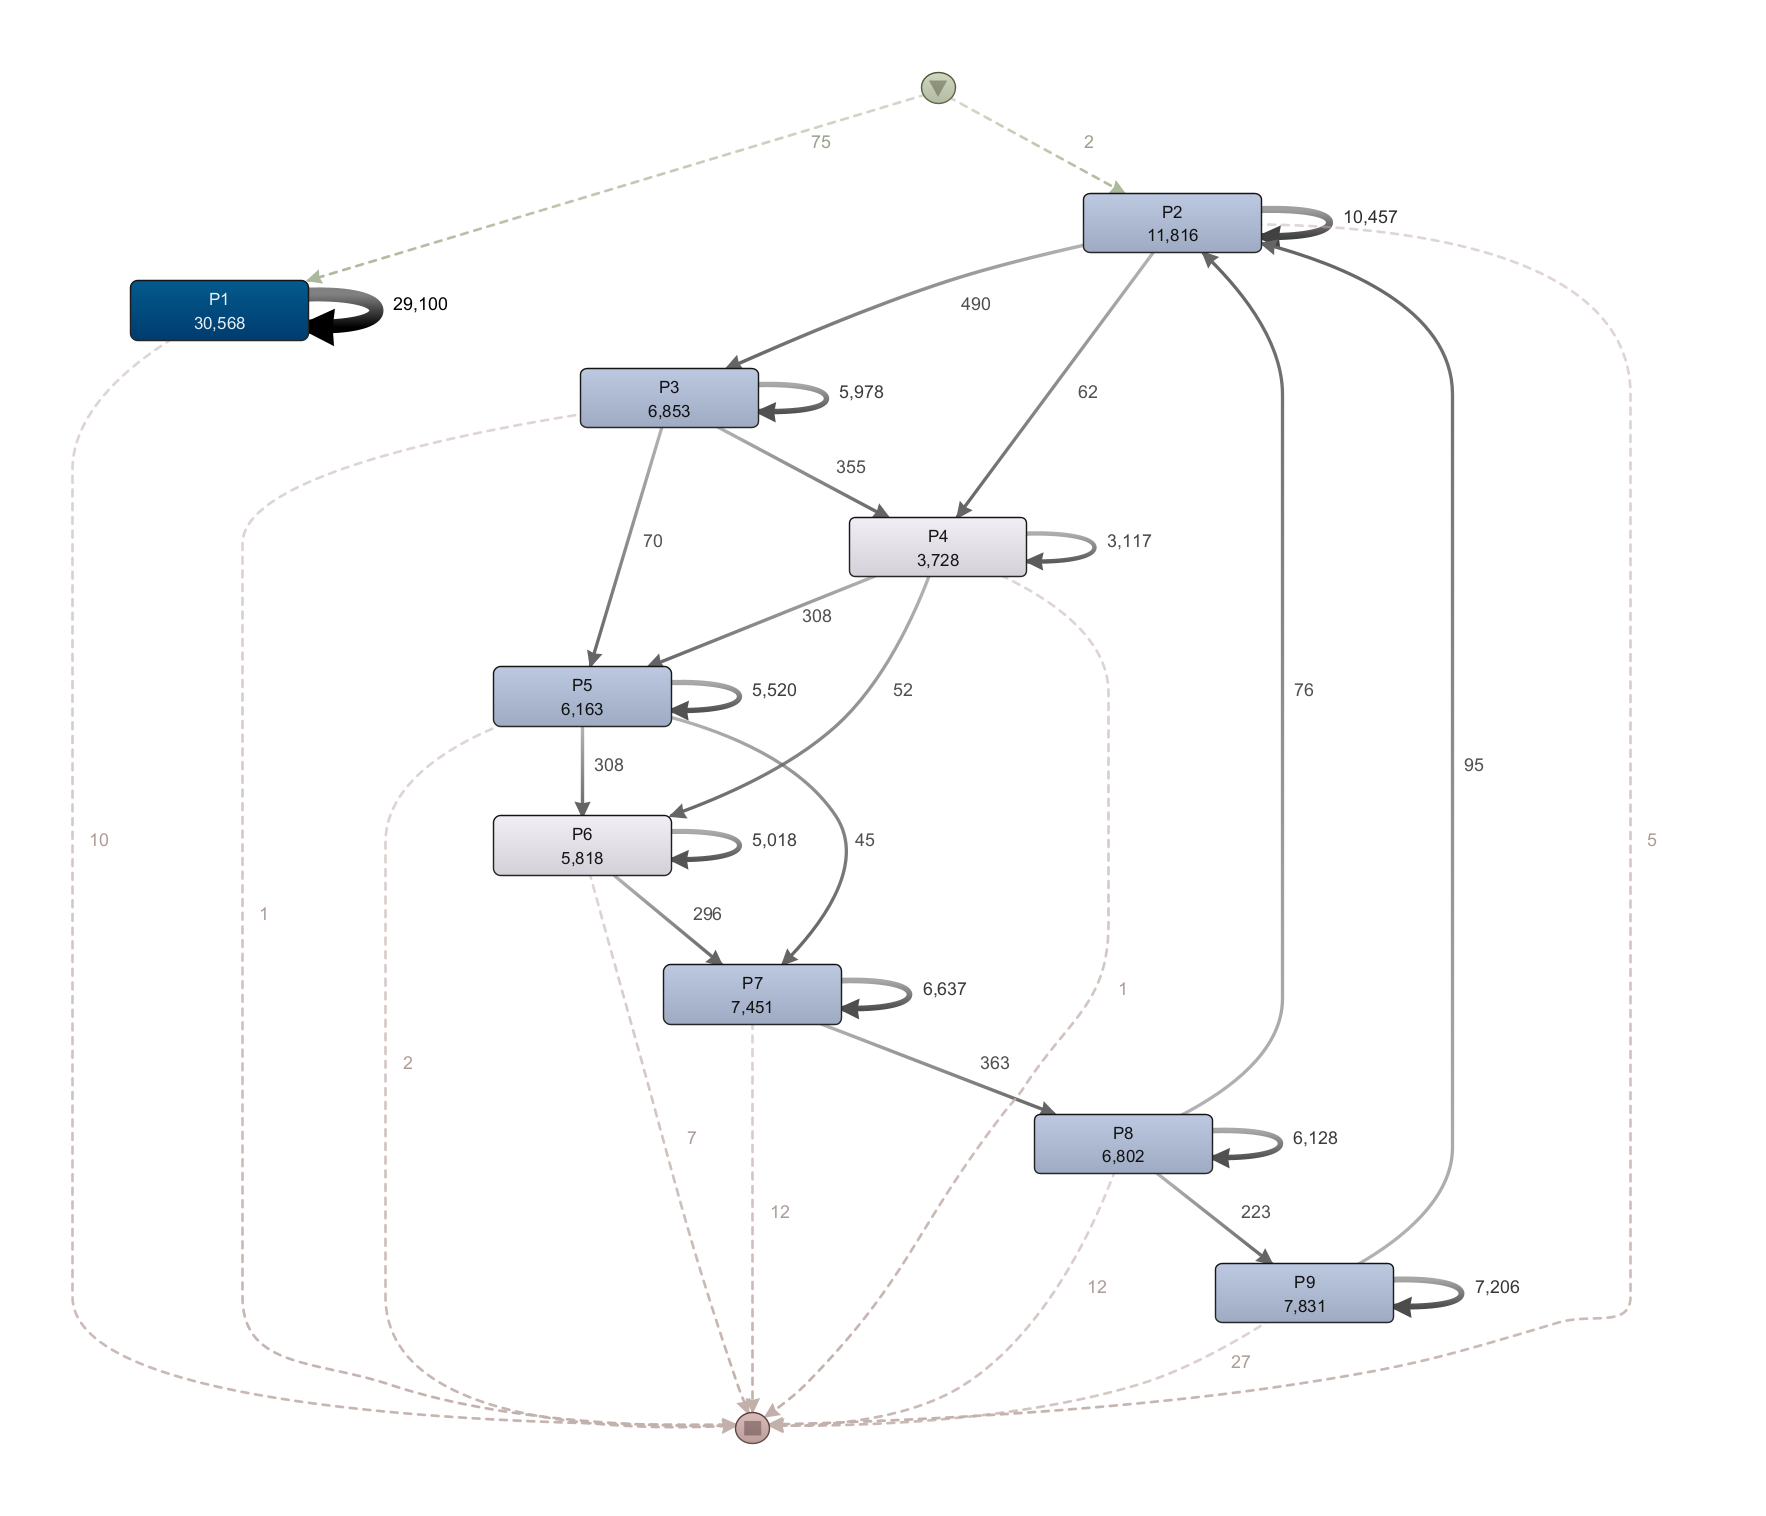
\includegraphics[width=\textwidth]{problems.png}
    \caption{Análisis de procesos del dataset (\texttt{Activity} problema y \texttt{CaseId} grupo). Contiene el $100\%$ de las actividades y el $80\%$ de los caminos.}
    \label{fig:problems}
\end{figure}

\begin{figure}[H]
    \centering
    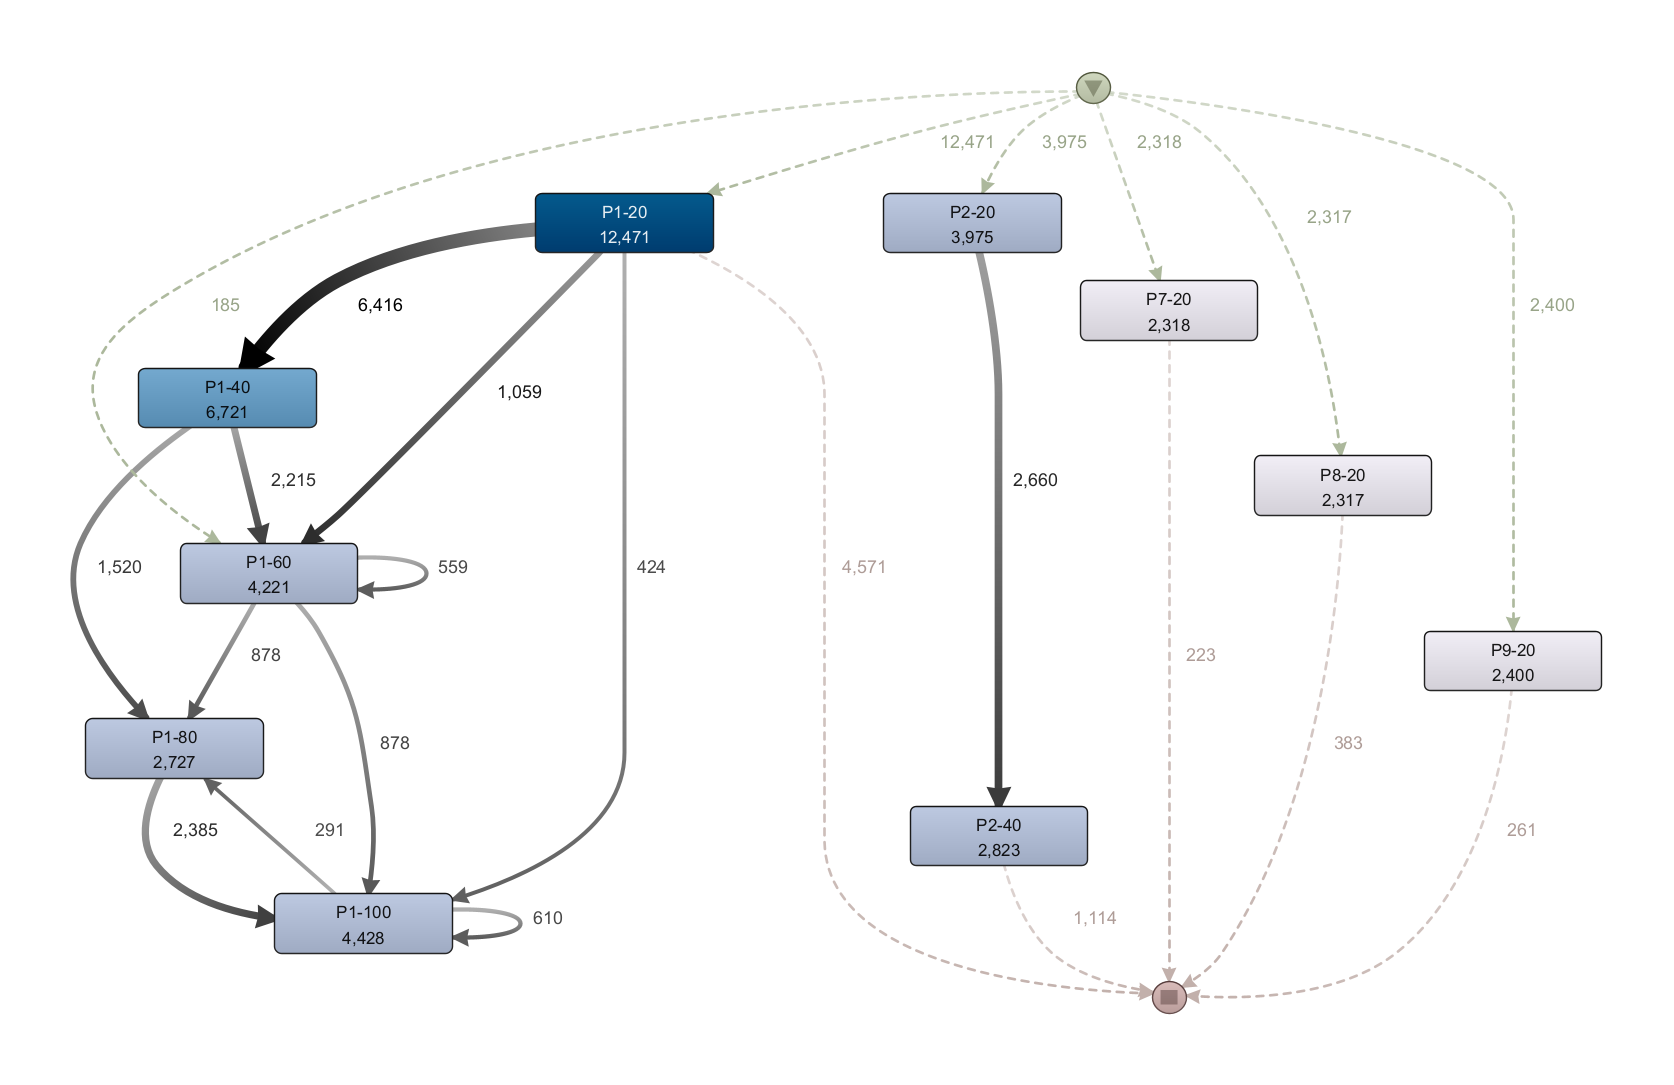
\includegraphics[width=\textwidth]{compound.png}
    \caption{Análisis de procesos del dataset (\texttt{Activity} problema-milestone y \texttt{CaseId} sesión). Contiene el $20\%$ de las actividades y el $20\%$ de los caminos.}
    \label{fig:compound}
\end{figure}

No obstante, a pesar de que tener una visión global del comportamiento de todos los grupos puede ayudar, nuestro objetivo final es poder caracterizar los comportamientos de los grupos y poder discernir, usando los datos del diagrama, si un grupo está en riesgo de obtener un rendimiento peor del esperado. Es por esto que nos será más interesante segmentar por grupos. Así pues, filtrando por el grupo \texttt{DBA 1516 P2 GA}, obtenemos los diagramas de las Figuras \ref{fig:problemsDBA1516P2GA} y \ref{fig:compoundDBA1516P2GA}.

\begin{figure}[H]
    \centering
    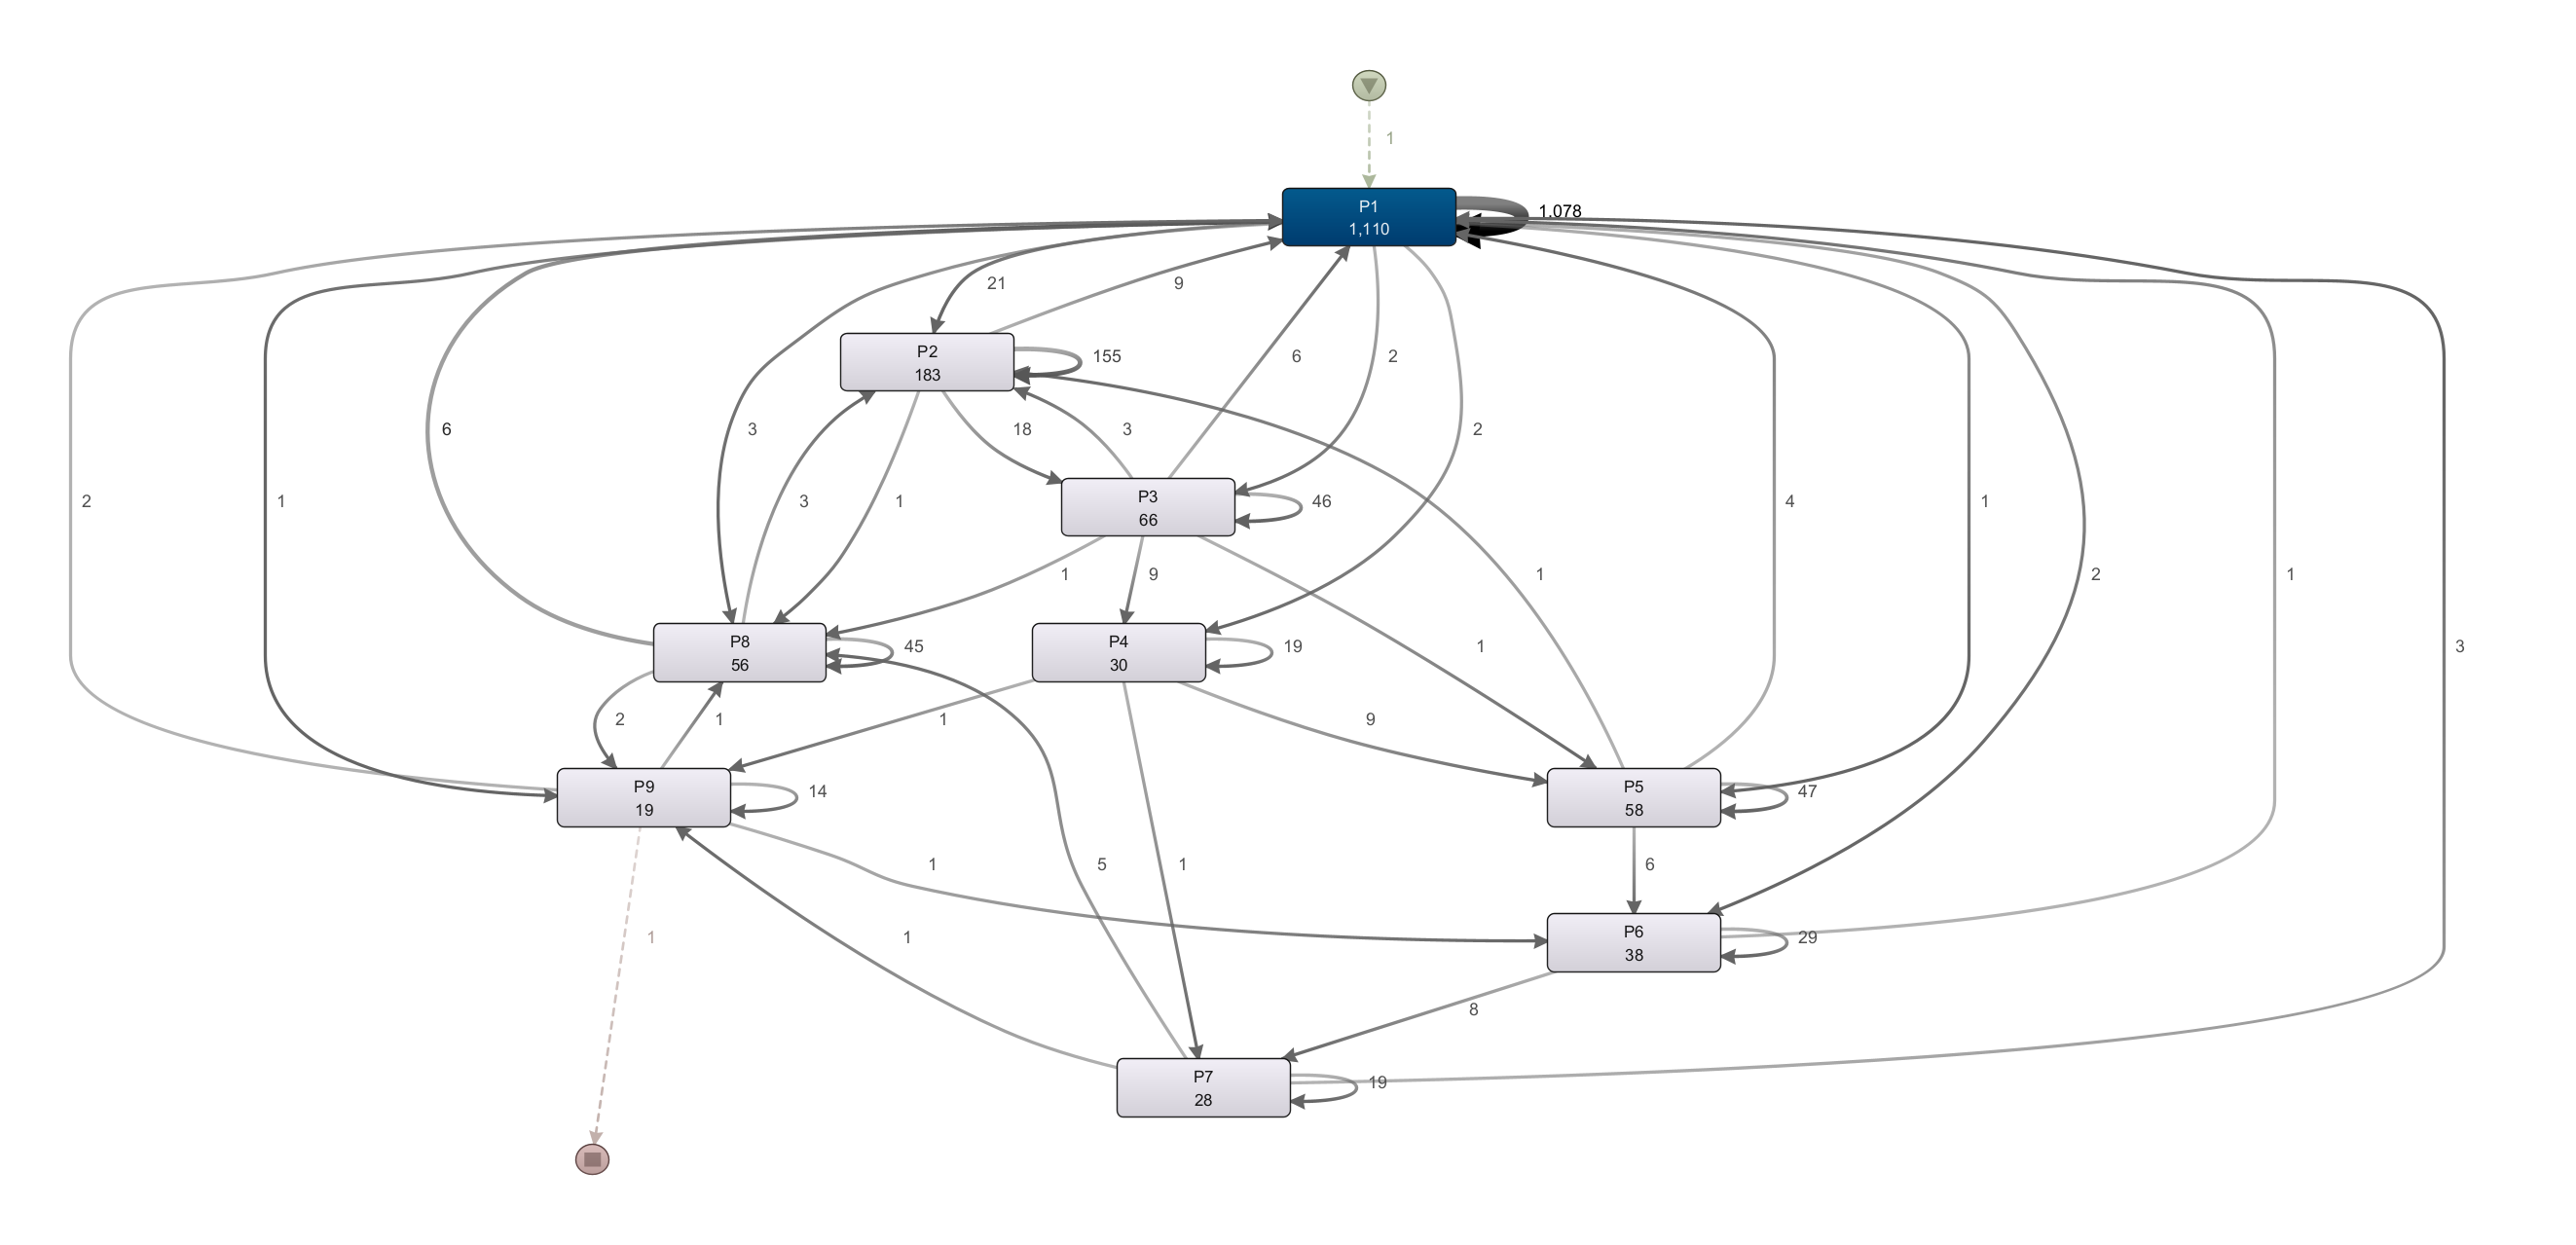
\includegraphics[width=\textwidth]{DBA1516P2GAProblems.png}
    \caption{Análisis de procesos del grupo \texttt{DBA 1516 P2 GA} (\texttt{Activity} problema y \texttt{CaseId} grupo). Contiene el $100\%$ de las actividades y el $100\%$ de los caminos.}
    \label{fig:problemsDBA1516P2GA}
\end{figure}

\begin{figure}[H]
    \centering
    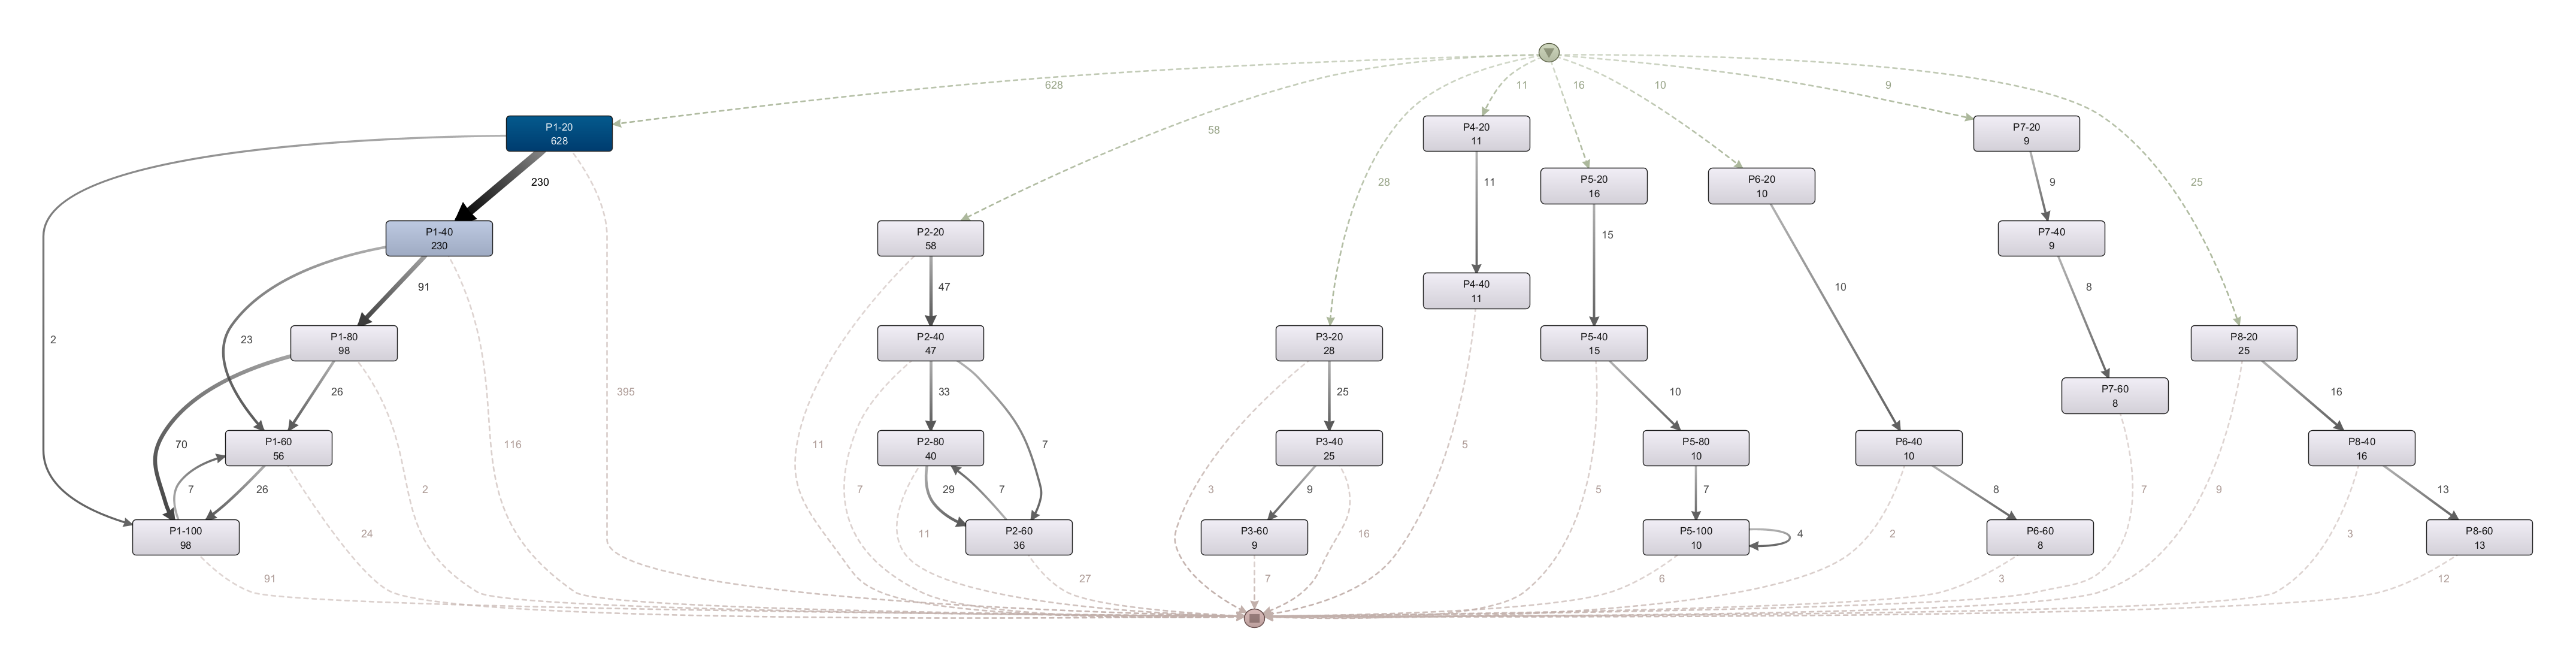
\includegraphics[width=\textwidth]{DBA1516P2GACompound.png}
    \caption{Análisis de procesos del grupo \texttt{DBA 1516 P2 GA} (\texttt{Activity} problema-milestone y \texttt{CaseId} sesión). Contiene el $60\%$ de las actividades y el $80\%$ de los caminos.}
    \label{fig:compoundDBA1516P2GA}
\end{figure}

Aunque Disco tiene mucho éxito y se pueden personalizar métricas e interpretaciones del conjunto de datos fuente, no se ajusta completamente a nuestros requerimientos para desvelar la estructura del comportamiento. Tras una larga experimentación con el programa Disco, se empiezan a ver sus limitaciones. En primer lugar, aunque Disco permite el filtrado de datos, si se quiere segmentar por grupos y extraer los procesos ocultos de cada uno de los grupos, hay que seleccionar el correspondiente grupo en el filtro, extraer los diagramas correspondientes e ir cambiándolo manualmente. Dado que tenemos un total de $77$ grupos de alumnos en los siete cursos académicos que forman parte del estudio (que pueden consultarse en las Tablas \ref{tab:groups1} y \ref{tab:groups2}), es inviable seguir usando el programa.

Así pues, en este trabajo fin de grado se ha implementado nuestra propia versión del programa, la herramienta de minería de procesos \emph{Graph Miner} en R, personalizada y adaptada a las necesidades del problema, basándose principalmente en la estructura principal de FuzzyMiner \cite{gunther2007fuzzy} con algunas adiciones menores.
\chapter{Implementación de la herramienta de Minería de Procesos \emph{Graph Miner}}\label{sec:chapterIV}
\addcontentsline{toc}{chapter}{Implementación de la herramienta de Minería de Procesos \emph{Graph Miner}}

\section{Uso de grafos como representación de los grupos}

Para dar una estructura de orden mínimo al comportamiento $B^g$, suponemos que es cierto lo siguiente: el resultado de la sesión $i$ depende en su mayor parte de lo ocurrido en la sesión $i-1$ o, como mucho, de cualquiera de las sesiones inmediatamente anteriores. Si aceptamos esta suposición, entonces $B^g$ tiene una estructura de orden parcial en la que cada sesión aparece conectada a la anterior.

Además, podríamos etiquetar estas relaciones con un número natural que indica el número de veces que esta relación se ha dado en $B^g$. De este modo se, obtiene el gráfico de la Figura \ref{fig:examplecycles}, un grafo conexo que describe el camino seguido por los estudiantes con un sentido claro de las transiciones de un estado a otro. Al igual que antes, también tenemos que la suma de las aristas entrantes a un nodo (o grado de entrada de dicho nodo) coincide con el número de veces que el nodo aparece en el registro. Nótese que como este estudio se centra en el éxito y el fracaso de los alumnos, el grafo de la Figura \ref{fig:examplecycles} es un grafo colapsado en el que sólo se distinguen dos tipos de sesiones: las que fracasan, es decir, las que alcanzan los hitos $1$ a $4$, y las que tienen éxito, es decir, las que alcanzan el hito final $5$. Así pues, notaremos a las sesiones fallidas por $^np_i^f$ y a las sesiones exitosas por $^np_i^s$, con $n \in \mathbb{N}$, como en la Figura \ref{fig:examples}, que continúa el ejemplo presentado en la Sección \ref{sec:initial}. Además, la matriz de adyacencia del segundo grafo puede verse en la Ecuación \ref{eq:matrix}.

\begin{figure}[H]
\centering
\subfloat[Grafo cíclico dirigido que captura las relaciones de precedencia entre las sesiones de la Tabla \ref{tab:sequence} ($20$ sesiones) obtenido colapsando los vértices de la misma en exitosas o fallidas. Los nodos con doble círculo representan sesiones en las que se ha resuelto un problema.]{\label{fig:examplecycles}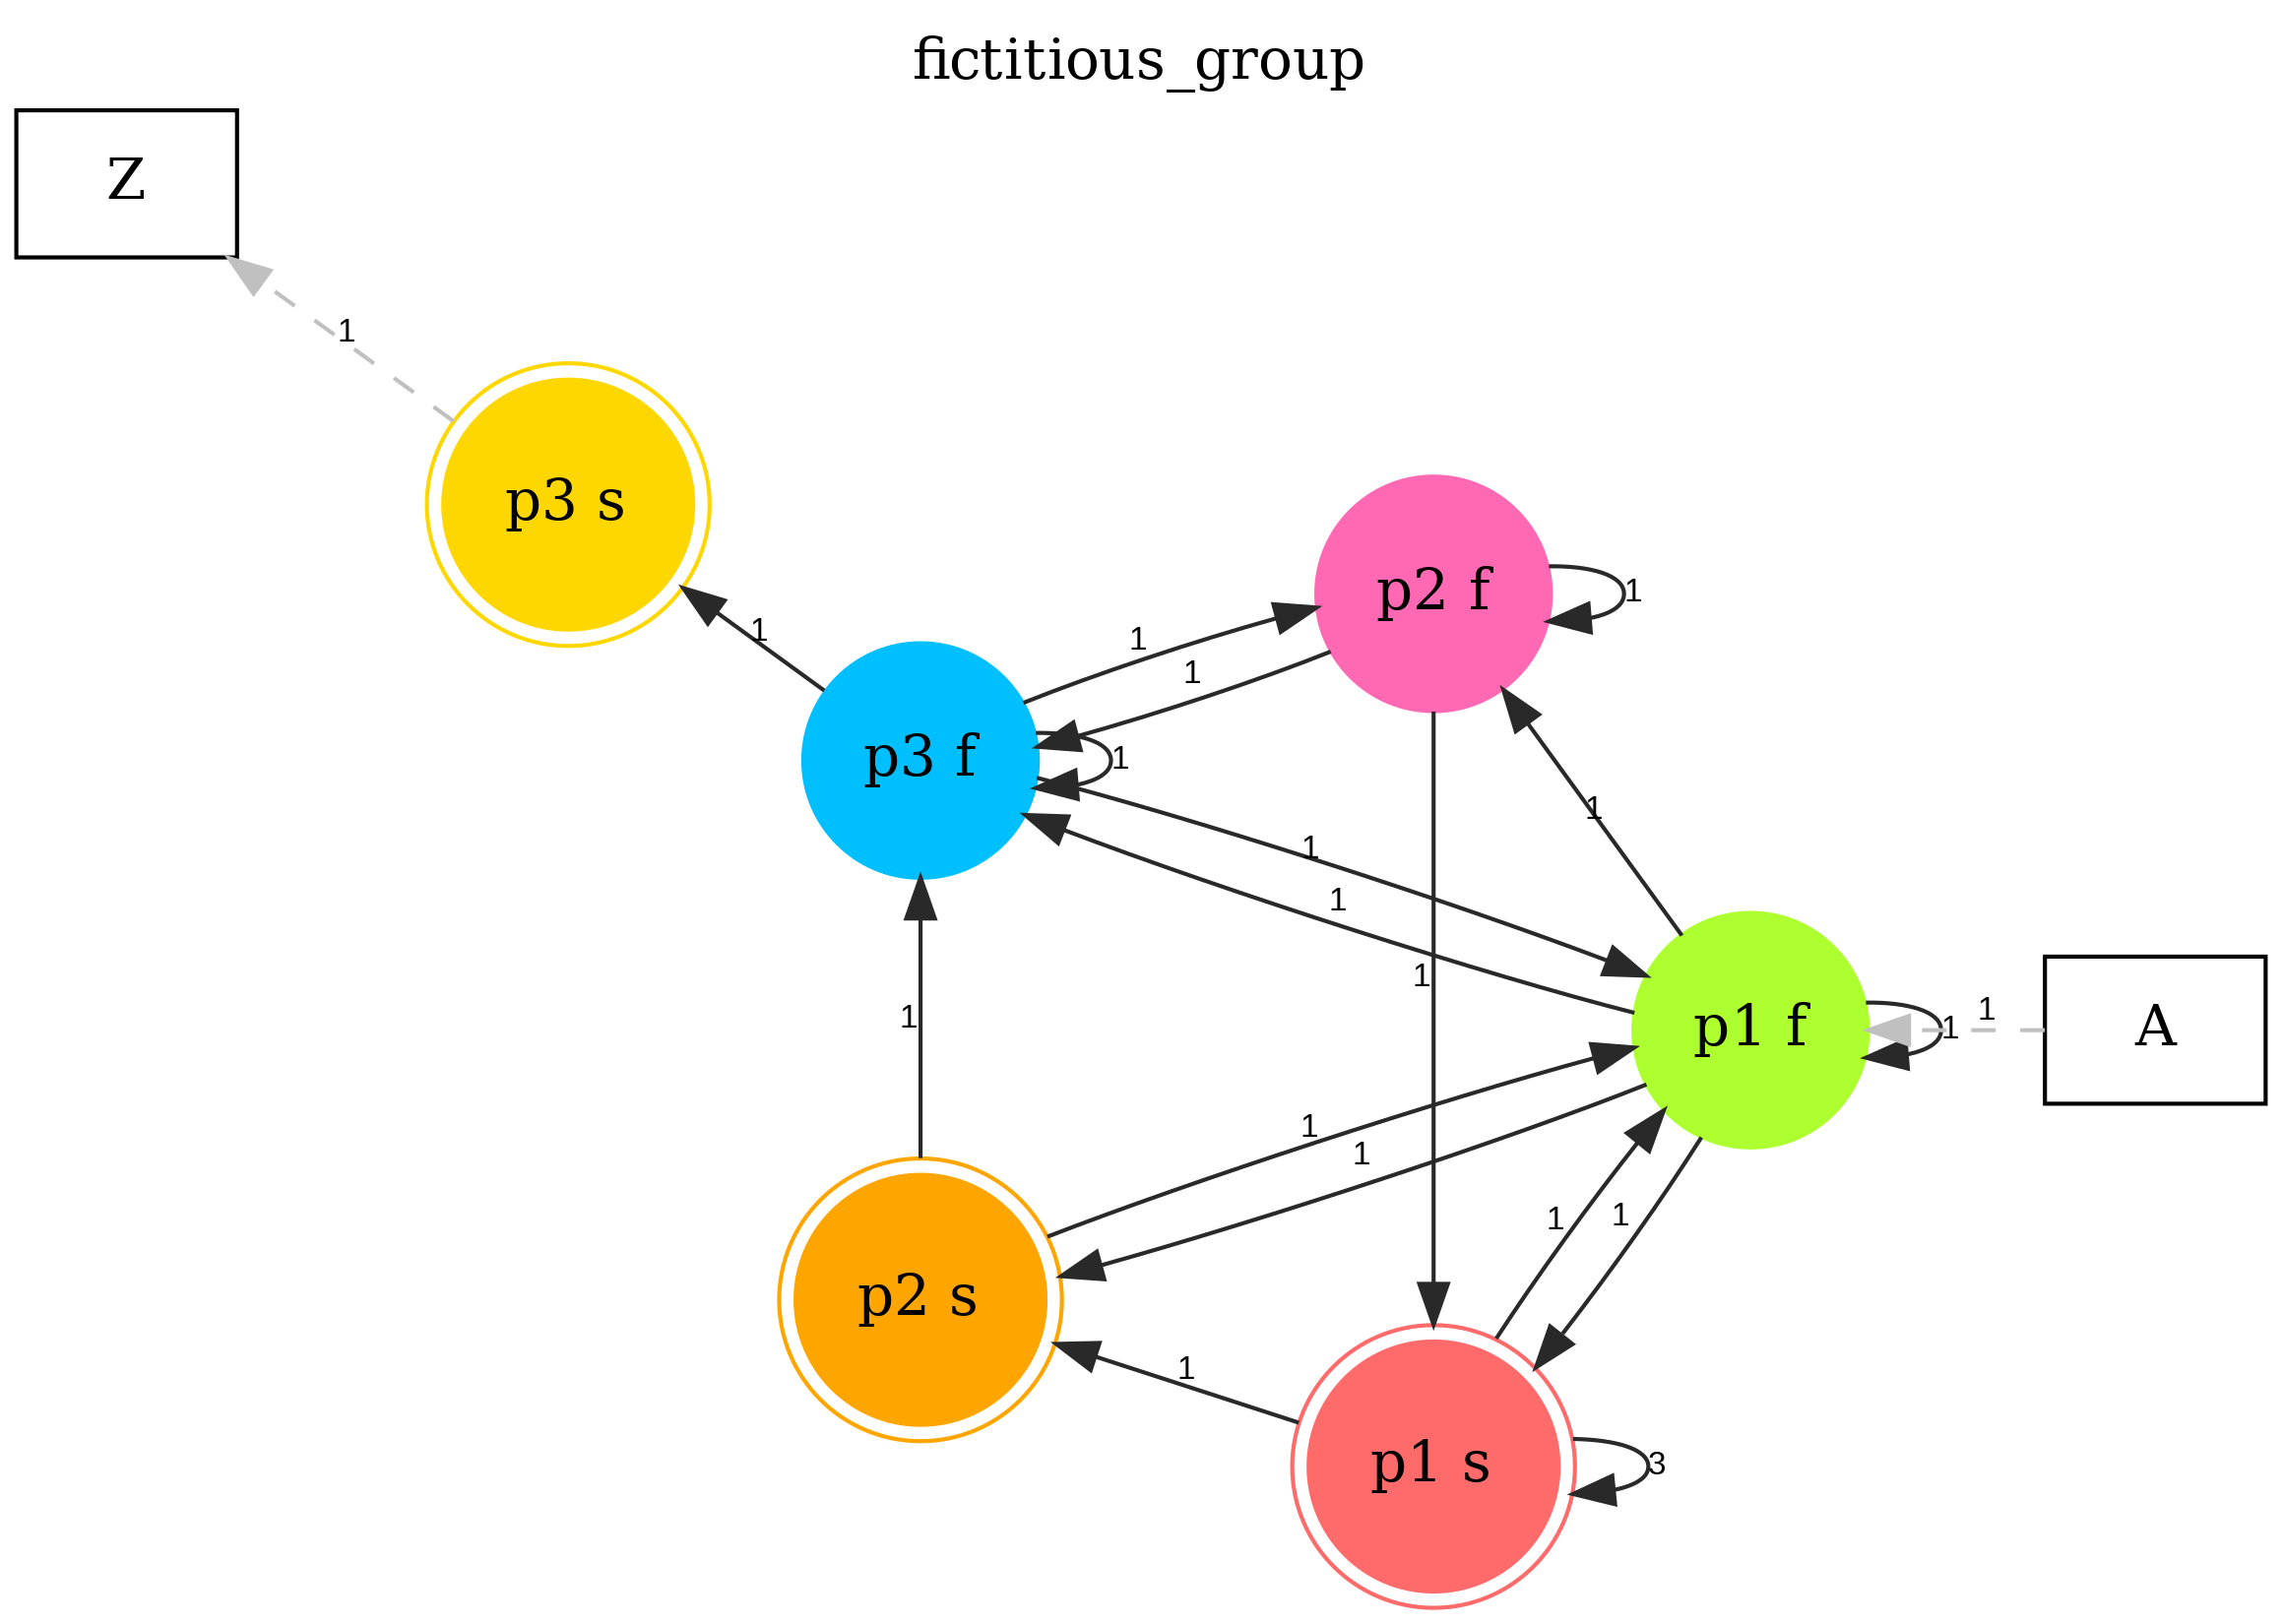
\includegraphics[width=0.47\textwidth]{implementación/examplecycles.png}}\qquad
\subfloat[El mismo grafo que el de la Figura \ref{fig:examplecycles} pero eliminando los ciclos
y manteniendo el grado de entrada de cada uno de los vértices.]{\label{fig:examplewithoutcycles}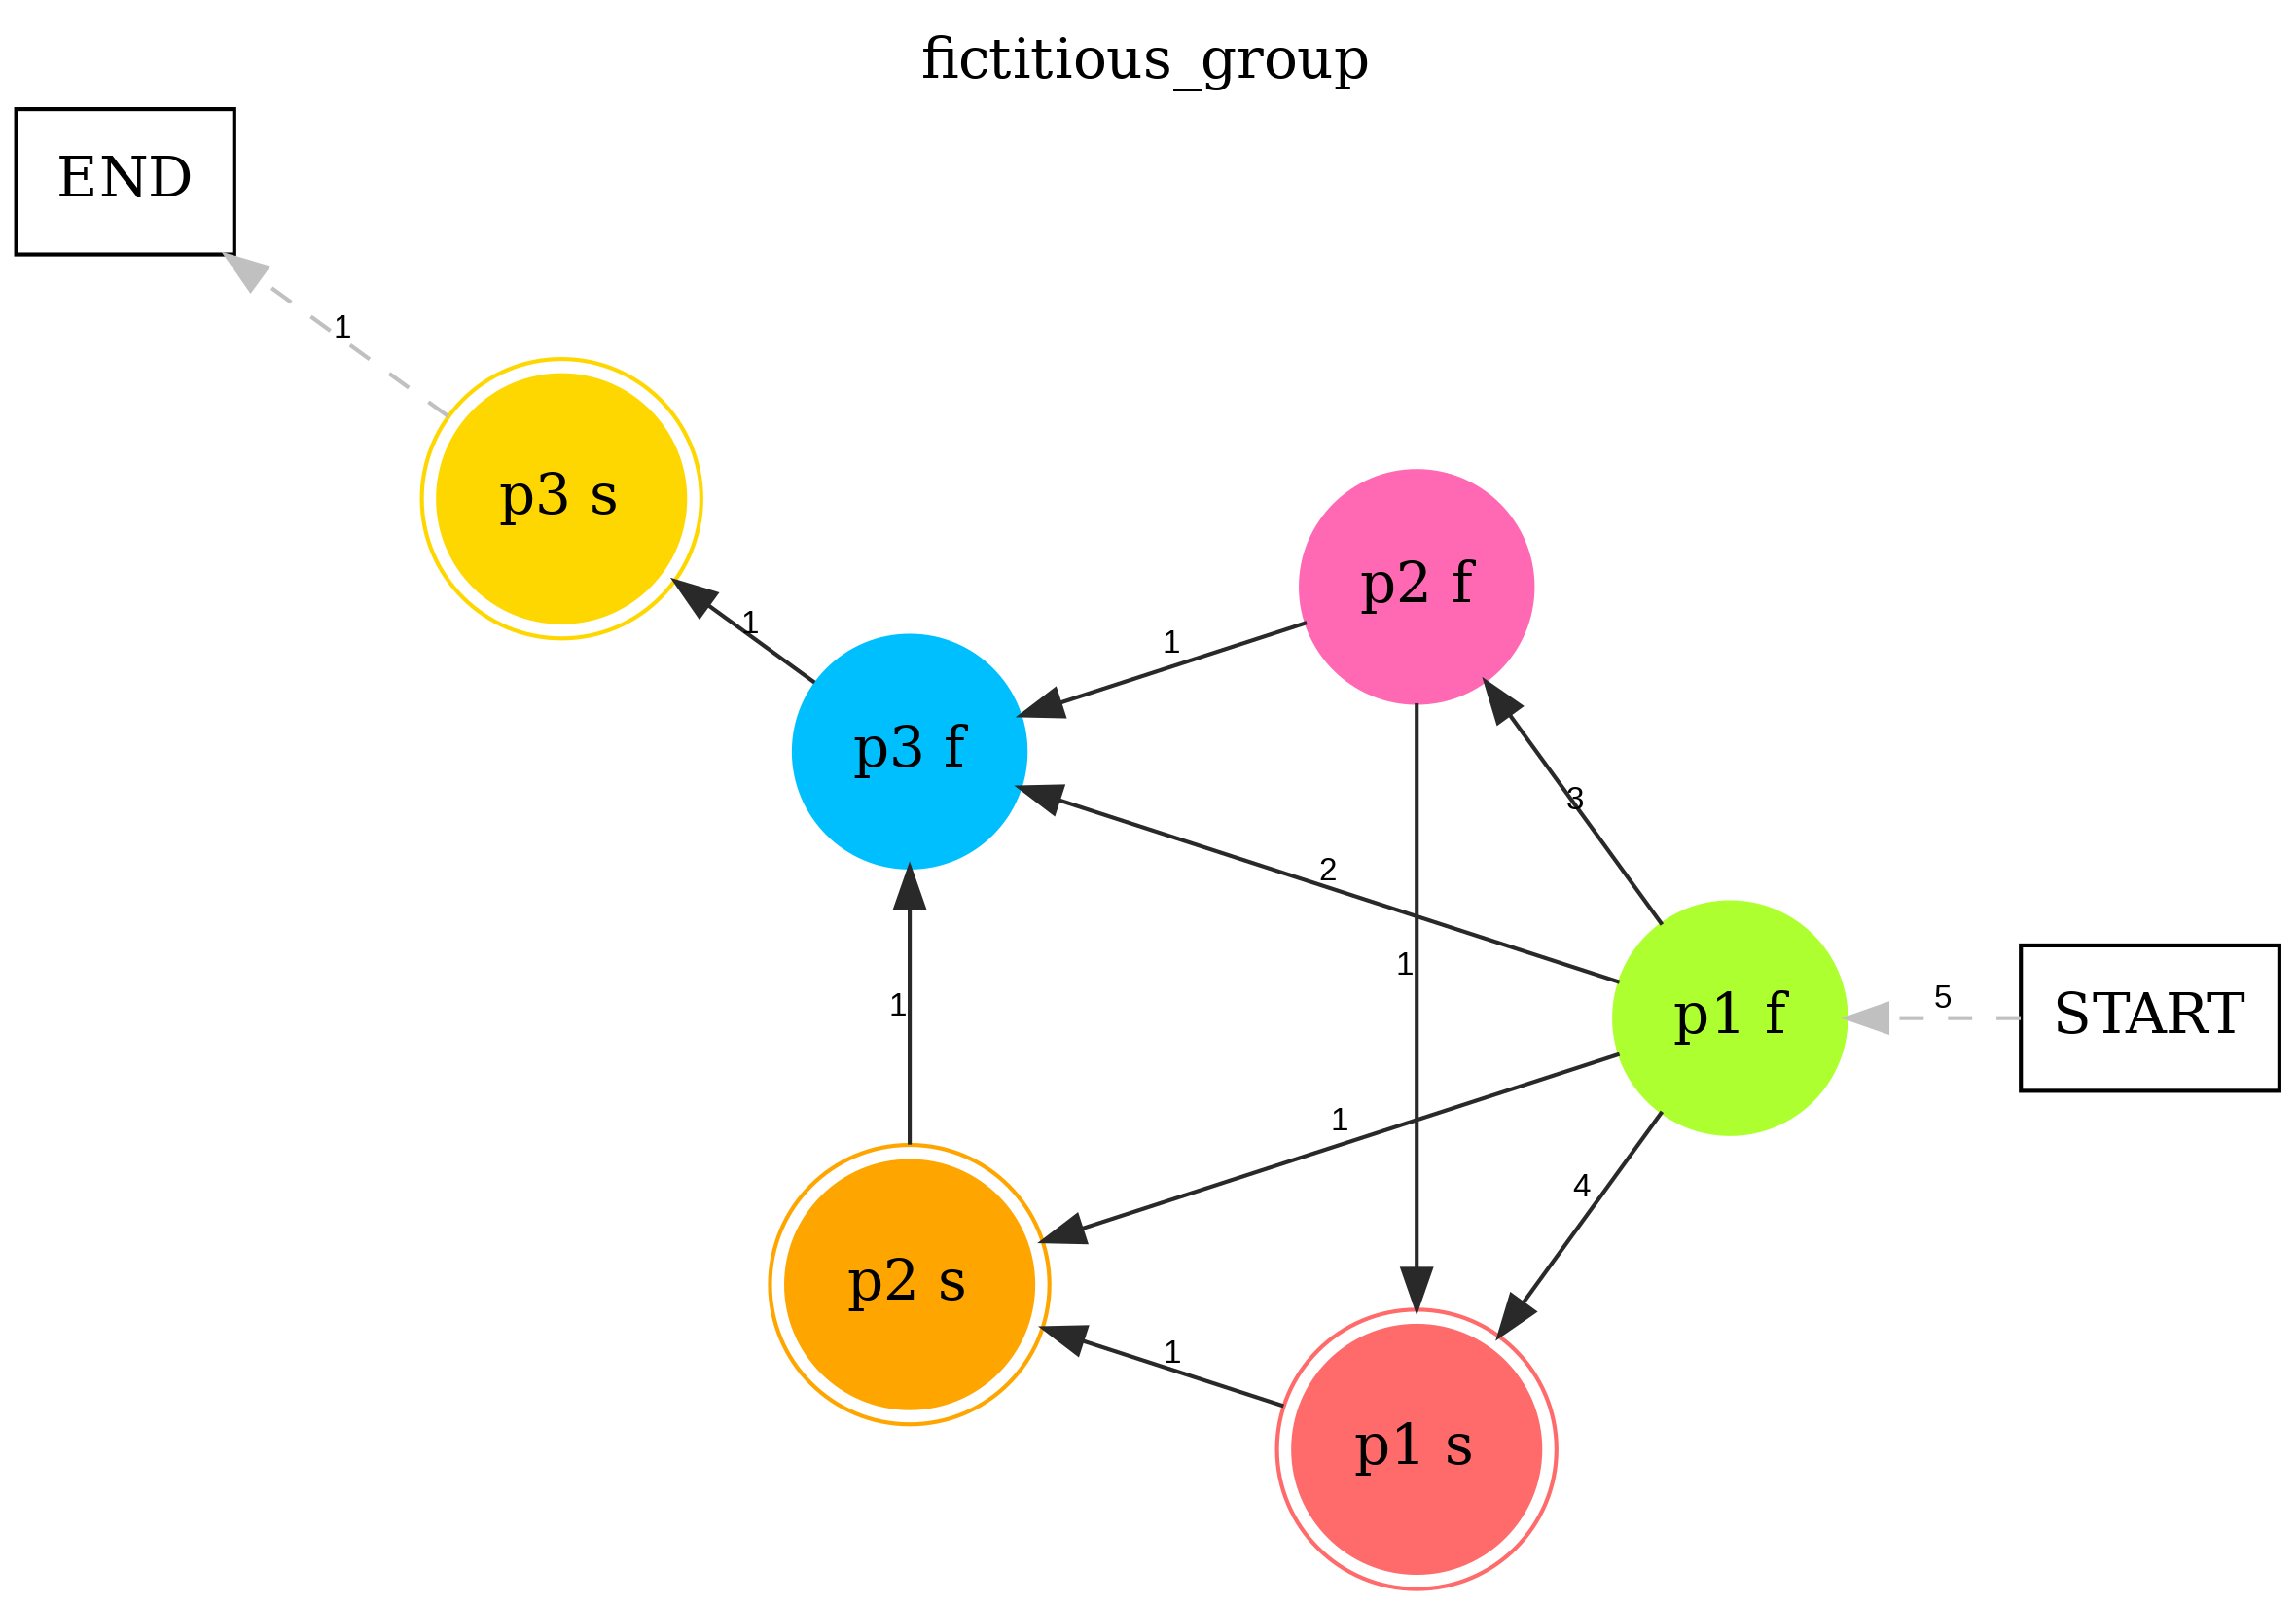
\includegraphics[width=0.47\textwidth]{implementación/examplewithoutcycles.png}}
\caption{Grafos resultantes de la continuación del ejemplo de la Sección \ref{sec:initial}.}
\label{fig:examples}
\end{figure}

\begin{equation}\label{eq:matrix}
\mathcal{A}^g = 
\left(
\begin{array}{c|cccccccc}
    & A & p_1^f & p_1^s & p_2^f & p_2^s & p_3^f & p_3^s & Z \\
  \hline
  A & \textbf{0} & 5 & 0 & 0 & 0 & 0 & 0 & 0 \\
  p_1^f & 0 & \textbf{0} & 4 & 3 & 1 & 2 & 0 & 0 \\
  p_1^s & 0 & 0 & \textbf{0} & 0 & 1 & 0 & 0 & 0 \\
  p_2^f & 0 & 0 & 1 & \textbf{0} & 0 & 1 & 0 & 0 \\
  p_2^s & 0 & 0 & 0 & 0 & \textbf{0} & 1 & 0 & 0 \\
  p_3^f & 0 & 0 & 0 & 0 & 0 & \textbf{0} & 1 & 0\\
  p_3^s & 0 & 0 & 0 & 0 & 0 & 0 & \textbf{0} & 1 \\
  Z & 0 & 0 & 0 & 0 & 0 & 0 & 0 & \textbf{0}
\end{array}
\right)
\end{equation}

Esta perspectiva nos permite ver $B^g$ como un grafo dirigido $G = (V^g,E^g)$ que capta la dinámica de un grupo mientras se esfuerza por resolver los distintos problemas que se le han planteado. Por lo tanto, el conjunto de eventos (problemas y estado de los mismos más un evento de inicio y otro de finalización) que los estudiantes han realizado es el conjunto de vértices del grafo:

\begin{equation}
V^g = \left\lbrace ^0A \right\rbrace \cup \left\lbrace ^sp_i^k \in B^g \right\rbrace \cup \left\lbrace Z \right\rbrace
\end{equation}

y cada par de eventos consecutivos se considera una arista del grafo:

\begin{equation}
E^g = \left\lbrace <x,y>, x = {}^sp_i^r, y = {}^tp_j^l, t = s+1, x,y \in B^g\right\rbrace
\end{equation}

que, de hecho, puede representarse como su matriz de adyacencia ponderada y nos permite representar el invariante grado de entrada.

\section{La matriz característica de un grupo}

Este grafo sigue siendo un grafo cíclico (Definición \ref{def:cyclic}) y, como estamos interesados en la representación más esencial del comportamiento de los estudiantes, se eliminarán esos ciclos quitando una cantidad mínima de aristas y conservando invariante el grado de entrada, obteniendo el grafo esencial de la Figura \ref{fig:examplewithoutcycles}, con su respectiva matriz de distancias (Ecuación \ref{eq:matrix}), que denominamos matriz característica (Definición \ref{def:adjacency}) del grupo $g$, $\mathcal{A}^g$. Esta matriz característica es una representación minimal de $B^g$ y a partir de ella se pueden extraer numerosas métricas, siendo la más importante una medida de la complejidad inherente a $B^g$.

Por lo tanto, $\mathcal{A}^g[x,y] = d > 0$ significaría que $x$ precede a $y$ $d$ veces en $B^g$. Así pues, cuanto mayor sea $d$, mayor será la influencia de $x$ sobre $y$ en términos del comportamiento codificado en $\mathcal{A}^g$. En aras de la simplicidad, además del uso de valores enteros para obtener una fila o columna, también se utilizarán los nombres identificativos de los nodos como, por ejemplo, se muestra en la Ecuación \ref{eq:example}.

\begin{equation}\label{eq:example}
\mathcal{A}[1,2] = \mathcal{A}[p_2^f,p_3^f] = 4
\end{equation}

Podría decirse que $\mathcal{A}^g$ contiene lo que podría haber sido la \emph{experiencia} de resolver todos los problemas, es decir, una especie de huella que codifica la relación entre fracaso y éxito y la fuerza de estas relaciones. Vale la pena decir que en todos los registros (Tabla \ref{tab:records}) todas estas matrices son diferentes entre sí. Se derivarán otras dos matrices de $\mathcal{A}^g$. En primer lugar, obtendremos una matriz de adyacencia característica integrada únicamente por ceros y unos a la que denotaremos $\mathcal{A}'$. Así pues, $\mathcal{A}'[r, c]$ será $1$ únicamente cuando $\mathcal{A}[r, c] > 0$. En segundo lugar, calcularemos la matriz de distancias mínimas que se obtendrá mediante la aplicación del algoritmo de caminos mínimos de Dijkstra, de modo que $\hat{\mathcal{A}}[r, c]$ contiene una especie de longitud de camino mínima entre los diferentes nodos del grafo en función del número de sesiones. Por tanto, estas estructuras son un punto de partida ideal desde el que decodificar la información sobre las experiencias de aprendizaje. En particular, nuestro principal interés será determinar si existe una relación entre esta estructura y el éxito o el fracaso de cada uno de los grupos de alumnos. Es decir, ¿un mal comportamiento de los alumnos produciría un grafo mal estructurado? Y viceversa, ¿las medidas estándar de calidad y entropía definidas puramente sobre grafos permiten detectar grupos en riesgo? La respuesta, resulta ser sí (Capítulo \ref{sec:chapterXIII}).

\section{Resultados obtenidos}

En esta sección se muestran los diferentes grafos obtenidos con la herramienta de Minería de Procesos \emph{Graph Miner}. Comparando las Figuras \ref{fig:DBA1516P2GA1} y \ref{fig:problemsDBA1516P2GA} vemos que los diagramas de la implementación propia y el original obtenido con Disco coinciden.

\begin{figure}[H]
    \centering
    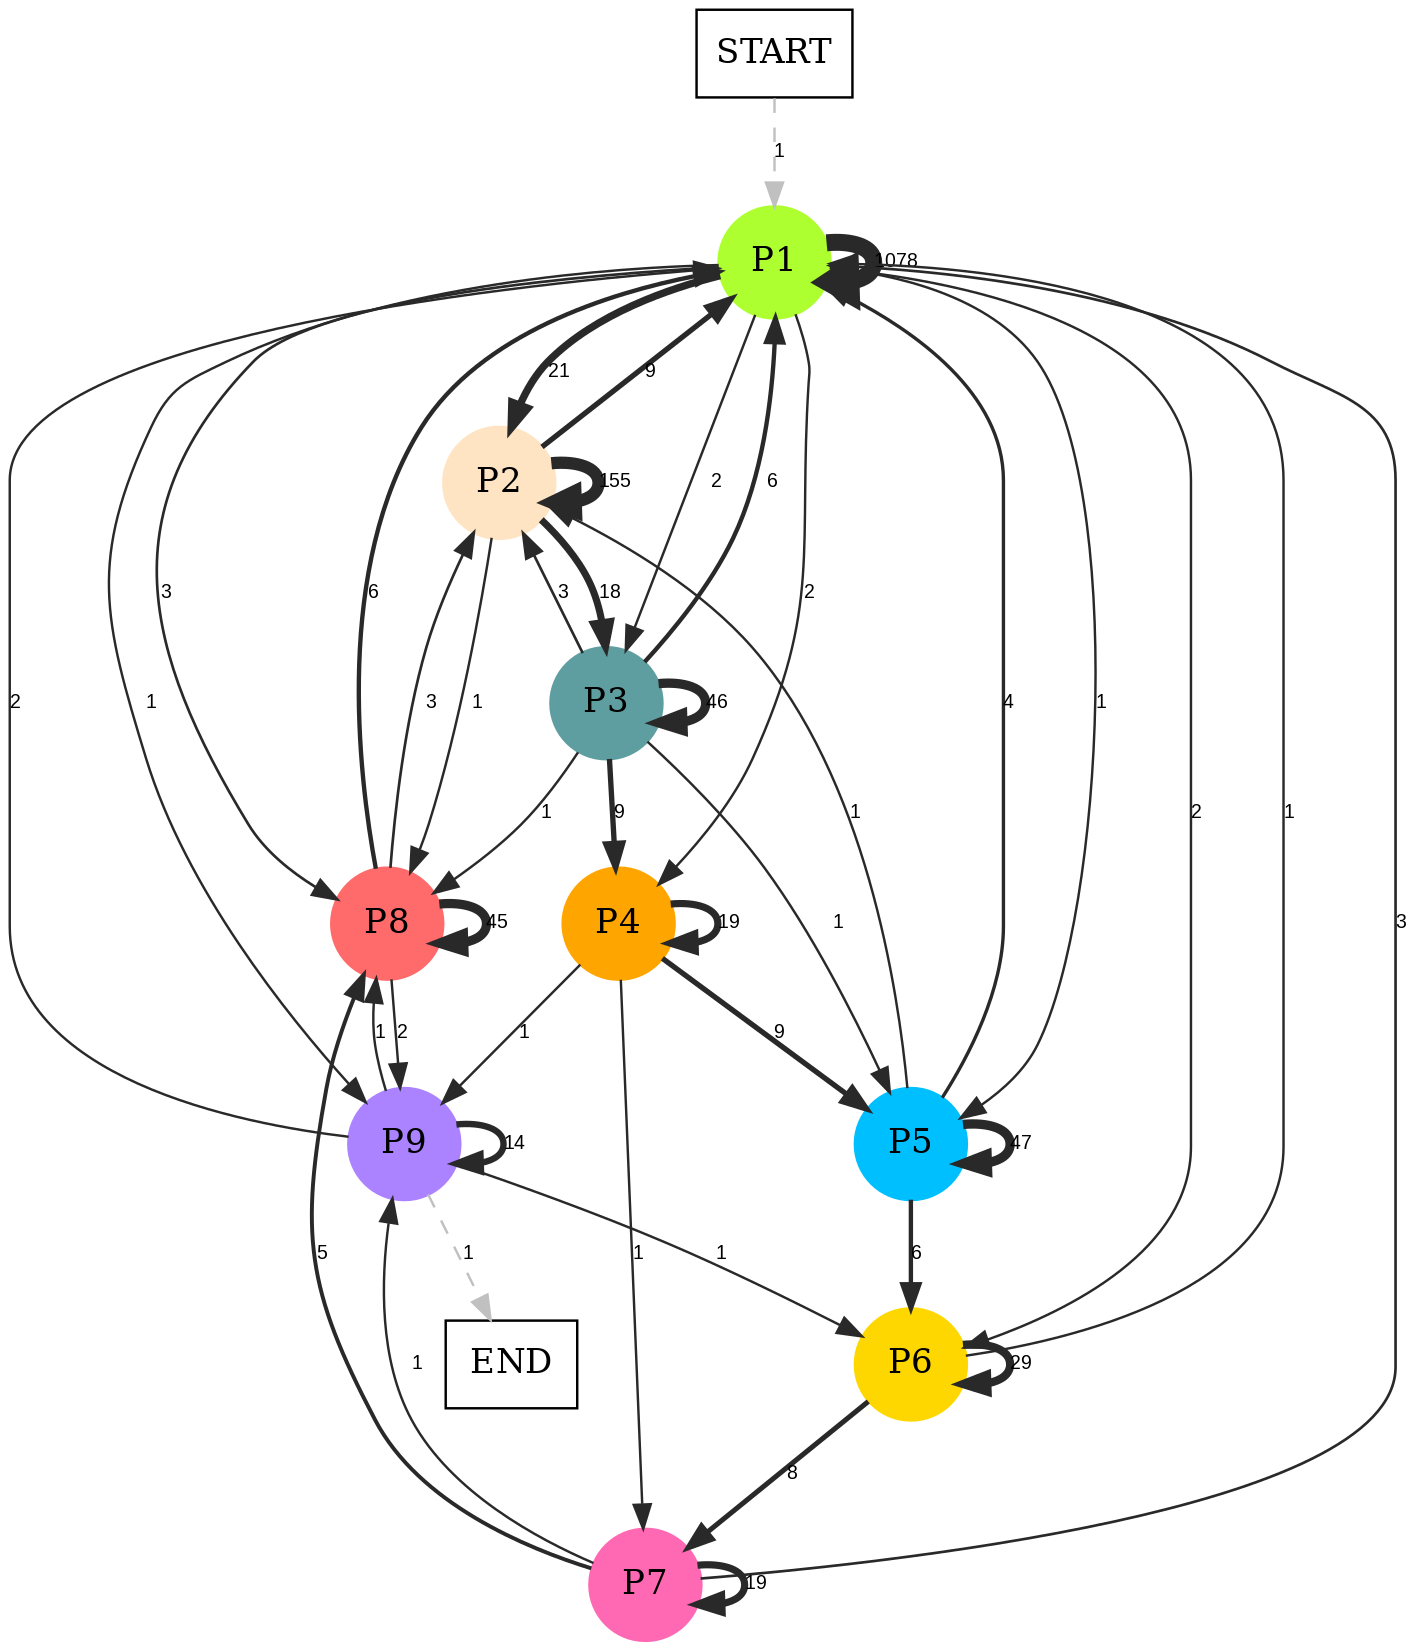
\includegraphics[width=0.5\textwidth]{DBA1516P2GA1.png}
    \caption{Análisis de procesos del grupo \texttt{DBA 1516 P2 GA} (\texttt{Activity} problema y \texttt{CaseId} grupo) obtenido con la implementación propia.}
    \label{fig:DBA1516P2GA1}
\end{figure}

Además, como podemos ver en la Figura \ref{fig:DBA1516P2GA2}, hemos obtenido el mismo diagrama que en el de la Figura \ref{fig:compoundDBA1516P2GA} con la salvedad de que hemos impedido el retorno a un estado anterior (el motivo se verá más adelante). Es decir, se han eliminado ciclos.

\begin{figure}[H]
    \centering
    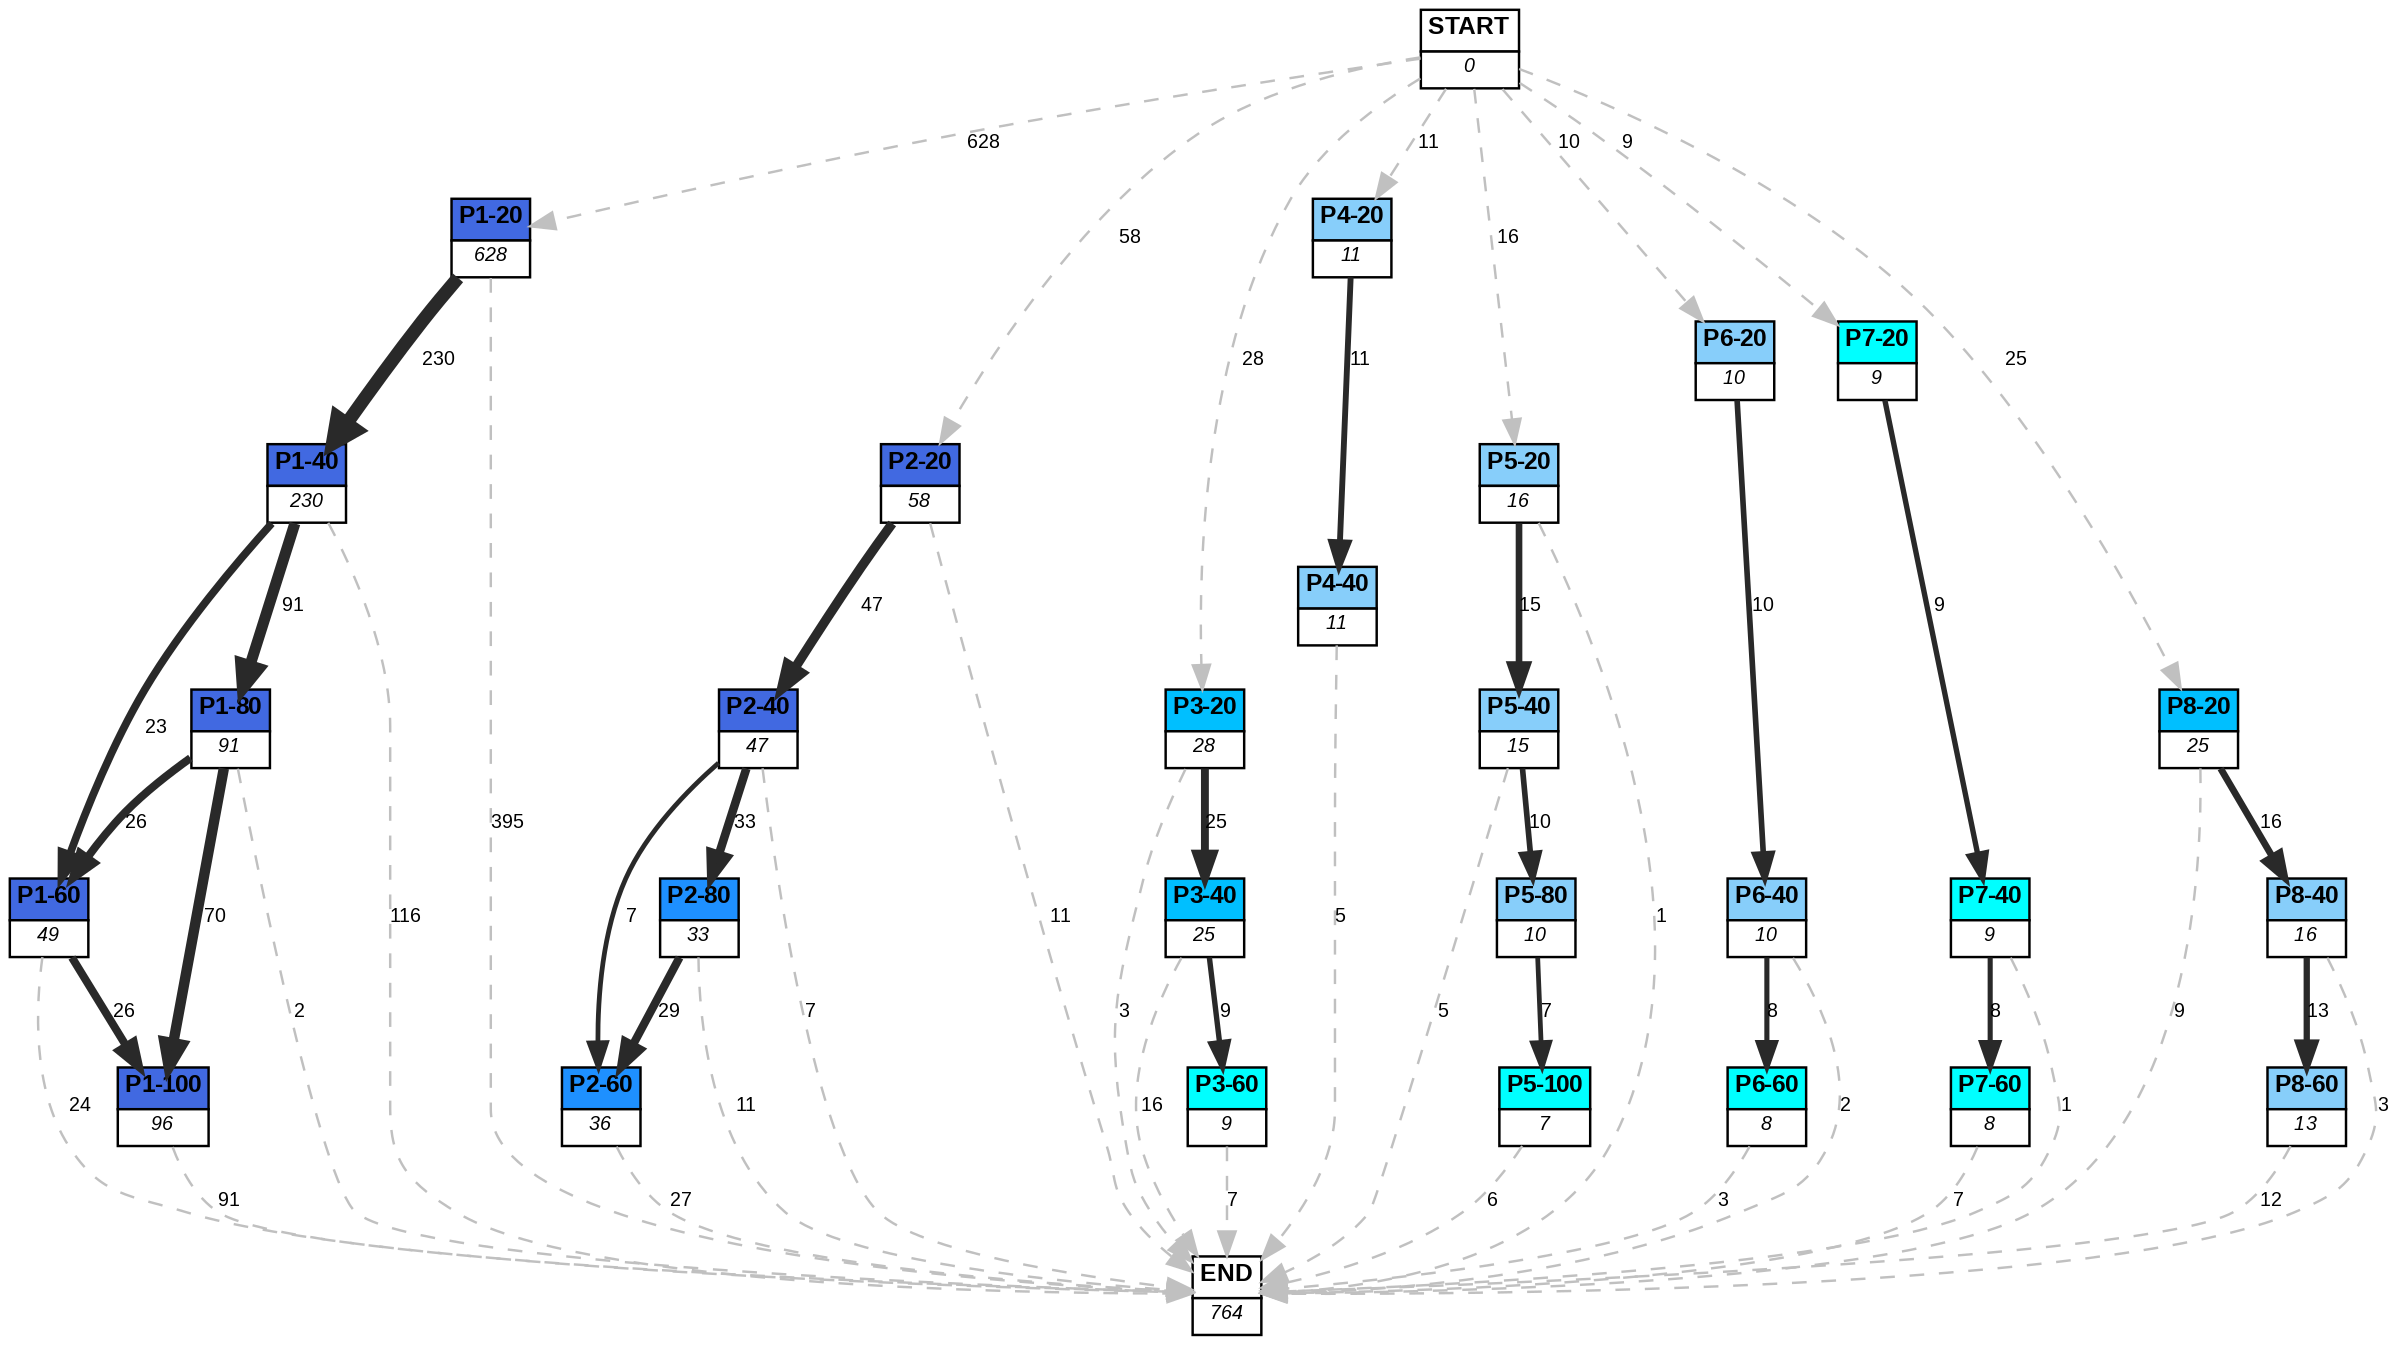
\includegraphics[width=\textwidth]{DBA1516P2GA2.png}
    \caption{Análisis de procesos del grupo \texttt{DBA 1516 P2 GA} (\texttt{Activity} problema-milestone y \texttt{CaseId} sesión) obtenido con la implementación propia.}
    \label{fig:DBA1516P2GA2}
\end{figure}

Además, se ha extendido la implementación de la herramienta de minería de procesos Disco \cite{gunther2012disco}, obteniendo otros diagramas que nos serán de mucha utilidad, como la agrupación en estados exitosos y fallidos (Figura) y una serie de grafos parciales considerando sólo la resolución hasta el problema $i$-ésimo, $i \in \left\lbrace 1,\dots,9 \right\rbrace$ (Figura).

A partir de ahora, estos diagramos tendrán la consideración de grafos. En particular, serán grafos dirigidos y operaremos con ellos como tales. En el siguiente capítulo se expondrán los conceptos básicos de grafos y principales resultados matemáticos que se usarán en este trabajo fin de grado.
\chapter{Teoría de grafos}
\addcontentsline{toc}{chapter}{Teoría de grafos}

En el ámbito de las matemáticas y las ciencias de la computación, se emplea el término \emph{grafo} (del griego \emph{grafos} que significa \emph{dibujo} o \emph{imagen}) para referirse a un conjunto de objetos llamados \emph{vértices} o \emph{nodos}, los cuales están unidos por enlaces conocidos como \emph{aristas} o \emph{arcos}. Estas conexiones representan las relaciones binarias que existen entre los elementos de un conjunto, y son objeto de estudio de la teoría de grafos.

\section{Grafos}

\begin{wrapfigure}{r}{0.4\textwidth}
\centering
\begin{tikzpicture}

% Posiciones fijas de los nodos
\node[circle, draw=black, fill=white] (1) at (0,0) {1};
\node[circle, draw=black, fill=white] (2) at (1,1) {2};
\node[circle, draw=black, fill=white] (3) at (1,-1) {3};
\node[circle, draw=black, fill=white] (4) at (-1,-1) {4};
\node[circle, draw=black, fill=white] (5) at (-1,1) {5};

% Arcos aleatorios
\draw[-, blue, line width=1pt] (1) to[bend left=20] (2);
\draw[-, green, line width=1pt] (2) to[bend left=20] (3);
\draw[-, red, line width=1pt] (3) to[bend left=20] (4);
\draw[-, orange, line width=1pt] (4) to[bend left=20] (5);
\draw[-, purple, line width=1pt] (5) to[bend left=20] (1);
\draw[-, violet, line width=1pt] (1) to[bend left=20] (3);

\end{tikzpicture}
\caption{Ejemplo de grafo simple.}
\label{fig:grafo1}
\end{wrapfigure}

En esta sección se introducirán las deficiones básicas que forman parte de la teoría de grafos.

\begin{definition}
Matemáticamente, un \emph{grafo} $G = (V,E)$ es una tupla de vértices $V$ y aristas $E$ que relacionan dichos vértices. Denominaremos  \emph{orden} del grafo al número de vértices del mismo ($|V|$). Por supuesto, siempre tendremos que $V \neq \emptyset$.
\end{definition}

\begin{exampleth}
El grafo dado en la Figura \ref{fig:grafo1} tiene conjunto de vértices $V=\left\lbrace 1,2,3,4,5 \right\rbrace$ y conjunto de aristas $E=\left\lbrace (1,2),(1,3),(2,3),(3,4),(4,5),(5,1) \right\rbrace$.
\end{exampleth}

\begin{definition}
Un \emph{vértice} o \emph{nodo} es la unidad fundamental de las que se componen los grafos. Los vértices en sí mismos se tratan como objetos indivisibles y sin propiedades. No obstante, pueden tener asociados una semántica dependiendo del contexto de aplicación del grafo. Por ejemplo, en el grafo \ref{fig:DBA1516P2GA2} un nodo representa la consecución de un objetivo de un problema.
\end{definition}

\begin{definition}
Una \emph{arista} representa una relación entre dos vértices de un grafo. Las aristas se denotan por $(u,v) \in E$ donde $u,v\in V$. Visualmente, se representan como las líneas que unen los vértices que forman parte de la definición de la misma.
\end{definition}

\begin{definition}
Un \emph{grafo podenderado} es un grafo cuyas aristas tienen un peso o valor asociado.

Formalmente, se puede definir como un trío ordenado $G=(V,E,W)$ donde $V=\left\lbrace v_1, \dots, v_n \right\rbrace$ es un conjunto de vértices, $E = \left\lbrace e_1, \dots, e_m \right\rbrace$ y $W = \left\lbrace w_1,\dots,w_m\right\rbrace$ es el conjunto de pesos asociados a cada arista.
\end{definition}

\deactivatequoting
\begin{figure}[H]
  \centering
\begin{minipage}[t]{0.45\linewidth}
\centering
\begin{tikzpicture}
  \node[circle, draw] (1) at (0,0) {1};
  \node[circle, draw] (2) at (2,0) {2};
  \node[circle, draw] (3) at (4,0) {3};
  \node[circle, draw] (4) at (0,2) {4};
  \node[circle, draw] (5) at (2,2) {5};
  \node[circle, draw] (6) at (4,2) {6};

  \draw[red, line width=1pt] (1) -- node[midway, above] {2} (2);
  \draw[blue, line width=1pt] (2) -- node[midway, above] {1} (3);
  \draw[green, line width=1pt] (3) -- node[midway, right] {3} (6);
  \draw[cyan, line width=1pt] (4) -- node[midway, below] {4} (5);
  \draw[orange, line width=1pt] (5) -- node[midway, below] {2} (6);
  \draw[purple, line width=1pt] (4) -- node[midway, right] {1} (1);
  \draw[magenta, line width=1pt] (2) -- node[midway, right] {4} (5);
\end{tikzpicture}
\caption{Ejemplo de grafo ponderado.}
\label{fig:grafo2}
\end{minipage}
\hspace{0.5cm}
\begin{minipage}[t]{0.45\linewidth}
\centering
\begin{tikzpicture}

% Posiciones fijas de los nodos
\node[circle, draw=black, fill=white] (1) at (0,0) {1};
\node[circle, draw=black, fill=white] (2) at (1,1) {2};
\node[circle, draw=black, fill=white] (3) at (1,-1) {3};
\node[circle, draw=black, fill=white] (4) at (-1,-1) {4};
\node[circle, draw=black, fill=white] (5) at (-1,1) {5};

% Arcos aleatorios
\draw[->, blue, line width=1pt] (1) to[bend left=20] (2);
\draw[->, green, line width=1pt] (2) to[bend left=20] (3);
\draw[->, red, line width=1pt] (3) to[bend left=20] (4);
\draw[->, orange, line width=1pt] (4) to[bend left=20] (5);
\draw[->, purple, line width=1pt] (5) to[bend left=20] (1);
\draw[->, violet, line width=1pt] (1) to[bend left=20] (3);

\end{tikzpicture}
\caption{Ejemplo de grafo dirigido.}
\label{fig:grafo3}
\end{minipage}
\end{figure}
\activatequoting

\begin{definition}
Un \emph{grafo no dirigido} es un grafo cuyas aristas representan relaciones simétricas y  carecen de sentido definido. Es decir, la arista $(u,v)$ es idéntica a la arista $(v,u)$. Es decir, las aristas no son pares ordenados sino conjuntos $\left\lbrace u,v \right\rbrace$ (o $2$-multiconjuntos) de vértices.

Un grafo no dirigido podrá tener, a lo más, $\frac{|V|^2}{2}$ aristas.
\end{definition}

\begin{definition}
Se denomina \emph{grafo dirigido} o \emph{digrafo} a aquellos grafos cuyas aristas tengan un sentido definido. En un digrafo, cada arista se representa como un par ordenado de dos vértices. Por ejemplo, $(u,v)$ denota la arista que va de $u$ hacia $v$ (desde el primer vértice hasta el segundo vértice).

Los grafos no dirigidos se pueden ver como un caso particular de los grafos dirigidos en tanto que son grafos dirigidos simétricos.

Mientras que en un grafo no dirigido se tiene que $E \subseteq \{x \in \mathcal{P}(V) : |x| = 2\}$ (es decir, $E$ es un conjunto de pares no ordenados de elementos de $V$), cuando el grafo es dirigido se tiene que $E$ es un conjunto de pares ordenados $(i,j) \in V \times V$.
\end{definition}

\begin{exampleth}
En la Figura \ref{fig:grafo3} se muestra un ejemplo de grafo dirigido mientras que en la Figura \ref{fig:grafo1} tenemos un ejemplo de grafo no dirigido.
\end{exampleth}

\begin{figure}[H]
    \centering
\begin{tikzpicture}
  \node[circle, draw] (1) at (0,0) {1};
  \node[circle, draw] (2) at (2,0) {2};
  \node[circle, draw] (3) at (4,0) {3};
  \node[circle, draw] (4) at (0,2) {4};
  \node[circle, draw] (5) at (2,2) {5};
  \node[circle, draw] (6) at (4,2) {6};

  \draw[red, line width=1pt] (1) -- (2);
  \draw[blue, line width=1pt] (2) -- (3);
  \draw[green, line width=1pt] (3) -- (4);
  \draw[yellow, line width=1pt] (4) -- (5);
  \draw[orange, line width=1pt] (5) -- (6);
  \draw[purple, line width=1pt] (6) -- (1);

  \draw[red, line width=1pt] (1) to [out=90, in=180, loop, distance=1cm] (1);
  \draw[blue, line width=1pt] (2) to [out=90, in=0, loop, distance=1cm] (2);
  \draw[green, line width=1pt] (3) to [out=90, in=0, loop, distance=1cm] (3);
  \draw[pink, line width=1pt] (5) to [out=90, in=90, loop, distance=1cm] (6);
  \draw[cyan, line width=1pt] (2) to [out=270, in=270, loop, distance=1cm] (3);
\end{tikzpicture}
	\caption{Ejemplo de multigrafo.}
	\label{fig:grafo4}
\end{figure}

\begin{definition}
Un \emph{grafo conexo} es un grafo en que todos sus vértices están conectados por un camino o por un semicamino dependiendo de si el grafo es no dirigido o dirigido.

De lo contrairo, si algún grafo no cumple la propiedad anterior se dirá que es \emph{disconexo}.
\end{definition}

\begin{definition}
Un \emph{bucle} es una arista que relacionado un vértice consigo mismo.
\end{definition}

\begin{definition}
En un grafo $G=(V,E)$, se dice que dos aristas son \emph{paralelas} o \emph{múltiples} si el vértice inicial y el vértice final de las mismas coinciden. 

Los grafos que permiten la existencia de bucles y aristas múltiples se denominan \emph{multigrafos}. Por el contrario, los grafos sin bucles y sin aristas paralelas se denominarán \emph{simples}.
\end{definition}

\begin{exampleth}
En la Figura \ref{fig:grafo2} tenemos un ejemplo de grafo ponderado.

En la Figura \ref{fig:grafo1} se muestra un ejemplo de grafo simple. Por otro lado, en la Figura \ref{fig:grafo4} podemos ver un multigrafo.
\end{exampleth}

\begin{definition}
En un grafo $G=(V,E)$ dos vértices se dirán \emph{adyacentes} (o \emph{vecinos}) si están relacionados por al menos una arista. Es decir, dos vértices $u,v \in V$ son adjacentes si $\exists e \in E$ tal que $e = (u,v)$.

La \emph{matriz de adyacencia} de un grafo es una matriz cuadrada de dimensión $|V| \times |V|$ que se utiliza como forma de representar las relaciones binarias entre los nodos del mismo. La denotaremos por $A = (a_{ij})_{1\leq i,j\leq |V|}$.

Si tenemos que $G$ es un grafo no dirigido, entonces $a_{ij} = 1$ y $a_{ji} = 1$ si el vértice $v_i$ es adyacente al vértice $v_j$ y $a_{ij} = a_{ji} = 0$ en caso contrario. Si el grafo $G$ es dirigido, entonces tendremos que $a_{ij} = 1$ si y sólo si existe $e \in E$ tal que $e = (v_i,v_j)$ y $a_{ij} = 0$ en caso contrario.

Por último, si tenemos un grafo ponderando, entonces se sustiuirá en valor de $1$ en los casos anteriores por el peso de las aristas correspondientes.
\end{definition}

\begin{exampleth}
Tenemos que la matriz de adyacencia del grafo de la Figura \ref{fig:grafo1} es:
\begin{equation}
\begin{pmatrix}
0 & 1 & 1 & 0 & 1\\
1 & 0 & 1 & 0 & 0\\
1 & 1 & 0 & 1 & 0\\
0 & 0 & 1 & 0 & 1\\
1 & 0 & 0 & 1 & 0
\end{pmatrix}
\end{equation}
\end{exampleth}

\begin{definition}
Sea $G=(V,E)$ un grafo no dirigido y sea $v \in V$ un vértice suyo. Se denomina grado del vértice $v$ al número de aristas incidentes al vértice y se denotará de ahora en adelante por $\text{deg}(v)$.

Al conjunto de todos los vértices adyacentes a un vértice dado se le denominará \emph{vecindad} del vértice en cuestión. Formalmente, la vecindad de un vértice $v \in V$ es el conjunto
\begin{equation}
N(v) = \left\lbrace u \in V | \left\lbrace v,u\right\rbrace \in E \right\rbrace
\end{equation}

Así pues, el grado de un vértice $v \in V$ puede definirse como el módulo de su vecindario: $\text{deg}(v) = |N(v)|$.

En el caso de los grafos dirigidos se distingue entre el \emph{grado de entrada} $\text{deg}^-(v)$ (número de aristas que tienen a $v$ como el vértice final) y el \emph{grado de salida} $\text{deg}^+(v)$ (número de ariastas que tienen a $v$ como vértice inicial). 
\end{definition}

% Meter Lema del apetrón de manos?

\begin{figure}[H]
\centering
\begin{tikzpicture}
  \foreach \x in {1,...,8}{
    \node[circle, draw] (\x) at ({45*(\x-1)}:2) {\x};
  }

  \foreach \x in {1,...,7}{
    \foreach \y in {\x,...,8}{
      \pgfmathsetmacro\randhue{rnd}
      \definecolor{mycolor}{hsb}{\randhue, 1, 1}
      \draw[mycolor, line width=1pt] (\x) -- (\y);
    }
  }
\end{tikzpicture}
\caption{Ejemplo de grafo completo.}
	\label{fig:grafo5}
\end{figure}

\begin{definition}
Un grafo en el que todos sus vértices tienen el mismo grado (de entrada, en el caso de los grafos dirigidos) se denomina \emph{regular}. Además, un grafo con vértices de grado $k$ se llamará $k$-regular.
\end{definition}

\begin{definition}
Un \emph{grafo completo} $G=(V,E)$ es un grafo no dirigido simple en el que para cada par de vértices $u, v\in V$ existe una arista $e \in E$ tal que $e = \left\lbrace u,v\right\rbrace$.

El \emph{grafo completo de $n$ vértices} se denotará por $K_n$. Así pues, $K_n$ tendrá $frac{n\cdot (n-1)}{2}$ aristas y es un grafo regular de grado $n-1$.
\end{definition}

\begin{figure}[H]
  \centering
\begin{minipage}[t]{0.45\linewidth}
\centering
\begin{tikzpicture}
  \foreach \x in {1,...,8}{
    \node[circle, draw] (\x) at ({45*(\x-1)}:2) {\x};
  }

  \foreach \x in {1,...,7}{
      \pgfmathsetmacro\randhue{rnd}
      \definecolor{mycolor}{hsb}{\randhue, 1, 1}
      \pgfmathtruncatemacro{\next}{\x + 1}
      \draw[mycolor, line width=1pt] (\x) -- (\next);
  }
  \pgfmathsetmacro\randhue{rnd}
  \definecolor{mycolor}{hsb}{\randhue, 1, 1}
  \draw[mycolor, line width=1pt] (8) -- (1);
\end{tikzpicture}
\caption{Ejemplo de grafo ciclo.}
	\label{fig:grafo6}
\end{minipage}
\hspace{0.5cm}
\begin{minipage}[t]{0.45\linewidth}
\centering
    \begin{tikzpicture}
  \foreach \x in {1,...,8}{
    \node[circle, draw] (\x) at ({45*(\x-1)}:2) {\x};
  }
  \node[circle, draw] (9) at (0,0) {9};

  \foreach \x in {1,...,7}{
      \pgfmathsetmacro\randhue{rnd}
      \definecolor{mycolor}{hsb}{\randhue, 1, 1}
      \pgfmathtruncatemacro{\next}{\x + 1}
      \draw[mycolor, line width=1pt] (\x) -- (\next);
      \draw[mycolor, line width=1pt] (\x) -- (9);
  }
  \pgfmathsetmacro\randhue{rnd}
  \definecolor{mycolor}{hsb}{\randhue, 1, 1}
  \draw[mycolor, line width=1pt] (8) -- (1);
  \draw[mycolor, line width=1pt] (8) -- (9);
\end{tikzpicture}
\caption{Ejemplo de grafo rueda.}
\label{fig:grafo7}
\end{minipage}
\end{figure}

\begin{definition}
Un \emph{grafo ciclo} o simplemente un \emph{ciclo} es un grafo que consiste en un camino simple cerrado. Esto es, hay un único camino en el que no se repite ningún vértice salvo el primero con el último.

Denotaremos a un grafo ciclo de $n$ vértices por $C_n$. Si consideramos que es un grafo no dirigido, cada vértice tendrá un vecindario de tamaño $2$ y, por tanto, será un grafo $2$-regular. Por el contrario, si tenemos un grafo dirigido, será un grafo $1$-regular.
\end{definition}

\begin{definition}
Un grafo rueda es un grafo de $n$ vértices (denotado usualmente por $W_n$) es un grafo que se obtiene al añadir un único vértice a un grafo ciclo de $n-1$ vértices, conectando el nuevo el vértice a todos los ya existentes. Es decir, el nuevo vértice será adyacente a todos los vértices del grafo $C_{n-1}$.
\end{definition}

\begin{exampleth}
En las Figuras \ref{fig:grafo5}, \ref{fig:grafo6} y \ref{fig:grafo7} podemos ver un grafo completo, un grado ciclo y un grafo rueda respectivamente.
\end{exampleth}

\begin{definition}
Diremos que un grafo es \emph{cíclico} si contiene al menos un grafo ciclo. Por el contrario, se dirá que un grafo es \emph{acíclico} si no contiene ningún ciclo.

No obstante, en este trabajo fin de grado nos centraremos en los llamados \emph{grafos dirigidos acíclicos} o \emph{DAG} (\emph{Directed Acyclic Graphs}, en inglés) que no son más que grafos dirigidos desprovistos de ciclos.
\end{definition}

\begin{figure}[H]
\centering
\begin{tikzpicture}

% Posiciones fijas de los nodos
\node[circle, draw=black, fill=white] (1) at (0,0) {1};
\node[circle, draw=black, fill=white] (2) at (1,1) {2};
\node[circle, draw=black, fill=white] (3) at (1,-1) {3};
\node[circle, draw=black, fill=white] (4) at (-1,-1) {4};
\node[circle, draw=black, fill=white] (5) at (-1,1) {5};

% Arcos aleatorios
\draw[->, blue, line width=1pt] (1) to[bend left=20] (2);
\draw[->, green, line width=1pt] (2) to[bend left=20] (3);
\draw[->, red, line width=1pt] (3) to[bend left=20] (4);
\draw[->, orange, line width=1pt] (4) to[bend left=20] (5);
\draw[->, violet, line width=1pt] (1) to[bend left=20] (3);

\end{tikzpicture}
\caption{Ejemplo de grafo acíclico dirigido con $5$ nodos.}
\label{fig:grafo8}
\end{figure}

\begin{exampleth}
En la Figura \ref{fig:grafo1} tenemos un grafo dirigido con ciclos o cíclico (contiene, por ejemplo, el $1$-$3$-$4$-$5$). Sin embargo, eliminado una de las aristas del mismo obtenemos el grafo de la Figura \ref{fig:grafo8}, que es acíclico. 
\end{exampleth}

\begin{definition}
Un grafo conexo acíclico no dirigido se denominará \emph{árbol}. Por otro lado, un \emph{árbol orientado} o \emph{poliárbol} será un grafo dirigido acíclico cuyo grafo no dirigido subyacente es un árbol. De otra manera, si cambiamos sus aristas dirigidas por no diridas, se obtendía un grafo no dirigido conexo y acíclico.
\end{definition}

\begin{definition}
Un \emph{árbol de expansión} de un grafo conexo no dirigido $G$ es un subgrafo suyo que es árbol y que contiene a todos sus vértices.

El \emph{número de árboles de expansión} de un grafo conexo $G$, habitualmente denotado por $t(G)$, es un invariante importante en la teoría de grafos. Éste puede obtenerse mediante el denominado \emph{Teorema de Kirchhoff}. Este teorema demuestra que el número de árboles de expansión de un grafo puede obtenerse en tiempo polinómico a partir del determinante de una submatriz de la \emph{matriz Laplaciana} del grafo. Más aún, nos dice que éste número es igual a cualquier cofactor de la matriz Laplaciana. El Teorema de Kirchhoff es una generalización de la \emph{fórmula de Cayley}, que proporciona el número de árboles de expansión en el caso de un grafo completo y que veremos a continuación.
\end{definition}

\begin{proposition}\label{prop:1}
Dado un grafo completo $K_n = (V,E)$ con $V=\left\lbrace v_1,v_2,\dots,v_n\right\rbrace$, la fórmula de Cayley establece que el número de árboles de expansión del mismo es $t(K_n) = n^{n-2}$.
\end{proposition}

En 1918, el alemán H. Prüfer obtuvo una elegante correspondencia biyectiva entre árboles etiquetados con $n$ vértices y sucesiones de longitud $n-2$, denominadas \emph{códigos de Prüfer}.

\begin{definition}
La definición del \emph{código de Prüfer} de un árbol $T = (V,E)$ no trivial, denotado por $P(T)$, es recursiva. Si $|V| = 2$ entonces $T$ consiste de una sola arista y $P(T) = \emptyset$. Supongamos ahora que el código de Prüfer de cualquier árbol con $n$ vértices está definido  y sea $T = (V = \left\lbrace v_1, v_2,\dots v_n, v_{n+1} \right\rbrace,E)$ un árbol con $n+1$ vértices. Sea
\begin{equation}
v = \min \left\lbrace i \in \left\lbrace 1,2,\dots,n,n+1 \right\rbrace | \text{ deg}(v_i) = 1\right\rbrace
\end{equation}
y sea $u$ el único vértice adyacente a $v$ en $T$. Por lo tanto, $T' = T - v$ es un árbol con $n$ vértices y $P(T-v)$ está bien definido por hipótesis de inducción. El código de Prüfer de $T$ se definirá de la siguiente forma:
\begin{equation}
P(T) = (u,P(T'))
\end{equation}
\end{definition}

\begin{figure}[H]
\centering
\begin{tikzpicture}
  \coordinate (A) at (90:2);
  \coordinate (B) at (18:2);
  \coordinate (C) at (-54:2);
  \coordinate (D) at (-126:2);
  \coordinate (E) at (162:2);

  \foreach \x/\label in {A/1, B/2, C/3, D/4, E/5}{
    \node[circle, draw] (\x) at (\x) {\label};
  }

  \draw[magenta, line width=1pt] (E) -- (B);
  \draw[blue, line width=1pt] (B) -- (C);
  \draw[cyan, line width=1pt] (D) -- (E);
  \draw[orange, line width=1pt] (E) -- (A);
\end{tikzpicture}
\caption{Ejemplo de árbol con $5$ nodos.}
\label{fig:arbol1}
\end{figure}

\begin{exampleth}
Consideremos el árbol de la Figura \ref{fig:arbol1}. Tenemos que el vértice de grado uno con la numeración más pequeña es el vértice $1$. Este vértice únicamente es adayacente al vértice número $5$. Así pues, $P(T) = (5,P(T-1))$. Cuando eliminamos el primer vértice, obtenemos que el vértice de grado uno de menor numeración es el $3$, cuyo único vértice adyacentes es el $2$, lo que conduce a que $P(T) = (5,2,P(T-\left\lbrace 1,3 \right\rbrace))$. Eliminando ahora este tercer vértice, tenemos que el vértice $2$ es el de menor numeración cuyo grado es $1$ y su único nodo adyacente es el número $5$. Esto hace que $P(T) = (5,2,5,P(T-\left\lbrace 1,3,2 \right\rbrace))$. Como $T-\left\lbrace 1,3 \right\rbrace$ es un árbol con dos vértices, $P(T-\left\lbrace 1,3 \right\rbrace) = \emptyset$ y $P(T) = (5,2,5)$.

Este ejemplo pone de manifiesto que no es necesario que todos los vértices aparezcan en el códgo de Prüfer y que pudiera ocurrir que un mismo vértice aparezca más de una vez en los mismos. De hecho, el número de veces que un vértice aparece en el código de Prüfer depende del grado de dicho vértice. Este resultado se verá en el siguiente Lema.
\end{exampleth}

\begin{proposition} % En realidad es un Lema
Sea $c_i$ el número de veces que aparece el número $i$ en el código de Prüfer de un árbol $T = (V=\left\lbrace 1,\dots, n \right\rbrace, E)$ con $n \geq 3$ vértices. Entonces $\text{deg}(i) = c_i +1$.
\end{proposition}

\begin{proof}
Si $n = 3$ entonces $P(T)$ consiste de un solo número, correspondiente al vértice de grado dos.

Supongamos ahora que el resultado es cierto para todo árbol $T = (V=\left\lbrace 1,\dots, n \right\rbrace, E)$ con $n \geq 3$ vértices. Sea $T' = (V'=\left\lbrace 1,\dots, n,n+1 \right\rbrace, E')$, $v = \min \left\lbrace i \in V' | \text{ deg}(i) = 1 \right\rbrace$ y sea $u$ el único vértice adyacente a $v$ en $T'$. Así pues, $P(T') = (u,P(T'-v))$. Para cada $i \in V'$ sea $b_i$ el número de veces que aparece $i$ en $P(T'-v)$. Por hipótesis de inducción, $\text{deg}_{T'-v}(i) = b_i + 1$.

Además, si $i \neq u$ entonces $c_i = b_i$ y $\text{deg}_{T'}(i) = \text{deg}_{T'-v}(i)$. Por lo tanto, en este primer caso, $\text{deg}_{T'}(i) = c_i + 1$. Por otra parte, si $i = u$ entonces $c_i = b_i + 1$ y $\text{deg}_{T'}(i) = \text{deg}_{T'-v}(i) +1$. Por lo tanto, $\text{deg}_{T'}(i) = b_i + 2 = c_i + 1$.
\end{proof}

El siguiente resultado muestra que el código de Prüfer define una función inyectiva del conjunto de árboles generadores con $n$ vértices al conjunto de palabras de longitud $n-2$ del alfabeto $\left\lbrace 1,2,\dots, n\right\rbrace$.

\begin{proposition}\label{prop:2}
Si $T$ y $T'$ son dos árboles con $n \geq 3$ vértices numerados tales que $P(T) = P(T')$, entonces $T = T'$.
\end{proposition}

\begin{proof}
Si $n = 3$, entonces $P(T)$ consiste de un solo número, correspondiente al único vértice de grado dos de $T$. Como $P(T) = P(T')$, este vértice también es el único vértice de grado dos de $T'$ y tenemos que $T = T'$.

Supongamos ahora que el resultado es cierto para cualesquiera dos árboles con $n$ vértices numerados. Sean ahora $T$ y $T'$ dos árboles con $n+1$ vértices numerados tales que $P(T) = P(T')$.  Sea $v$ el mínimo elemento de $\left \lbrace 1,\dots,n,n+1\right \rbrace$ que no aparece en $P(T)$. Por el lema anterior $\text{deg}_T (v) = 1$ y $\text{deg}_{T'} = 1$. Así pues, existe un único $u$ tal que $u$ es adyacente a $v$ en $T$ y existe un único $u'$ tal que $u'$ es adyacente a $v$ en $T'$. De ahí obtenemos que $P(T) = (u,P(T-v))$ y que $P(T') = (w,P(T-v'))$. Como $P(T) = P(T')$, se sigue que $u = u'$ y, por lo tanto, $P(T-v) = P(T'-v')$. Por lo que, por hipótesis de inducción, $T-v = T'-v$. Concluimos así que $T=T'$.
\end{proof}

A continuación veremos que a cada palabra de longitud $n-2$ del alfabeto $\left\lbrace 1,2,\dots,n \right\rbrace$ le corresponde un árbol cuyo código de Prüfer es esa palabra.

\begin{proposition}\label{prop:3}
Sea $n \geq 3$. Si $L = (u_1,u_2,\dots,u_{n-2})$ es una lista cuyos elementos pertenecen al conjunto $V = \left\lbrace 1,\dots,n\right\rbrace$, entonces existe un árbol con vértices numerados (o etiquetado) $T$ tal que $P(T) = L$.
\end{proposition}

\begin{proof}
Si $n=3$ entonces $L = (u_1)$ y $T$ es la trayectoria de longitud dos cuyo vértice interno es $u_1$.

Supongamos ahora que el resultado es cierto para toda lista de longitud $n-2$. Sea $L = (u_1,u_2,\dots,u_{n-1})$ una lista de longitud $n-1$. Sea $v$ el elemento más pequeño de $V$ que no aparece en $L$. Por hipótesis de inducción existe un árbol $T' = (V',E')$ con conjunto de vértices $V_{T'} = \left\lbrace 1,\dots,n+1 \right\rbrace - \left\lbrace v \right\rbrace$, tal que $P(T') = (u_2,u_3,\dots,u_{n-1})$. Sea $e$ la arista que une a $v$ con $u_1$ y sea $T = (V' + v, E' + e)$. Tenemos que $T$ es un árbol y que $P(T) = (u_1,P(T')) = L$ tal y como se quería demostrar.
\end{proof}

El siguiente ejemplo pone en práctica el procedimiento descrito en el lema anterior para construir un árbol generador cuyo código de Prüfer sea igual a una lista dada.

\begin{exampleth}
Consideremos la lista $(3,5,3,1)$. La longitud de esta lista es $4$, por lo que corresponde a un árbol con conjunto de vértices $V = \left\lbrace 1,2,3,4,5,6 \right\rbrace$. El primer vértice que no aparece en la lista es $2$, el cual deber ser adyacente al vértice $3$ (Figura \ref{fig:arbol2}). Consideremos ahora la sublista $(5,3,1)$, el primer vértice del conjunto $\left\lbrace 1,3,4,5,6 \right\rbrace$ (obtenido al eliminar el vértice $2$) que no aparece en la lista es el $4$, que debe ser adyacente al vértice $5$. Análogamente, el primer vértice del conjunto $\left\lbrace 1,3,5,6 \right\rbrace$ que no aparece en la sublista $(3,1)$ es el $5$, el cual debe ser adyacente al vértice $3$, y el primer vértice del conjunto $\left\lbrace 1,3,6 \right\rbrace$ que no aparece en la sublista $(1)$ es el $3$, el cual debe ser adyacente al vértice $1$. Finalmente, obtenemos la lista vacía y el conjunto $\left\lbrace 1,6 \right\rbrace$, lo cual indica que el vértice $1$ debe ser adyacente al vértice $6$. La Figura \ref{fig:graforesult} es el árbol asociado a la lista $(3,5,3,1)$.
\end{exampleth}

\begin{figure}[H]
\centering
\begin{tikzpicture}
  \coordinate (A) at (90:2);
  \coordinate (B) at (30:2);
  \coordinate (C) at (-30:2);
  \coordinate (D) at (-90:2);
  \coordinate (E) at (-150:2);
  \coordinate (F) at (150:2);

  \foreach \x/\label in {A/1, B/2, C/3, D/4, E/5, F/6}{
    \node[circle, draw] (\x) at (\x) {\label};
  }

  \draw[blue, line width=1pt] (B) -- (C);
  \draw[green, line width=1pt] (C) -- (E);
  \draw[magenta, line width=1pt] (D) -- (E);
  \draw[orange, line width=1pt] (C) -- (A);
  \draw[purple, line width=1pt] (F) -- (A);
\end{tikzpicture}
\caption{Ejemplo de árbol con $6$ nodos.}
\label{fig:arbol2}
\end{figure}

Finalmente, se procederá a demostrar la fórmula de Cayley \ref{prop:1}:
\begin{proof}
Si $n = 1$ o $n = 2$ el resultado es trivialmente cierto. Si $n \geq 3$ de las Proposiones \ref{prop:2} y \ref{prop:3} se sigue que existe una correspondencia biyectiva entre el conjunto de árboles generadores con $n$ vértices y el conjunto de palabras de longitud $n-2$ del alfabeto $\left\lbrace 1,2,\dots,n \right\rbrace$. Como el número de palabras de longitud $n-2$ de un alfabeto con $n$ elementos es $n^{n-2}$, entonces hay $n^{n-2}$ árboles de expansión distintos de un grafo completo con $n$ vértices.
\end{proof}

A continuación, se introducirá el concepto de matriz laplaciana de un grafo que, junto con el Teorema de Kirchhoff nos permitirá calcular el número de árboles de expansión de un grafo arbitrario.

\begin{definition}
La matriz laplaciana (también conocida como matriz de admitancia o matriz de Kirchhoff) es una representación matricial de un grafo muy utilizada en la Teoría espectral de grafos, cuyo objetivo es el estudio de las propiedades de los grafos en relación de los polinomios caracterísicos, valores y vectores propios de las matrices asociadas a los mismos.

Para un grafo simple $G$ con vértices $V = (v_1,\dots,v_n)$ los elementos de la matrix laplaciana $L_{n\times n}$ se definen como sigue:

\begin{equation}
L_{i,j} = 
\begin{cases}
    \text{deg}(v_i) & \text{si } i=j \\
    -1 & \text{si } i\neq j \text{ y }v_i \text{ es adyacente a }v_j\\
    0 & \text{en cualquier otro caso}
\end{cases}
\end{equation}

Equivalentemente, se tiene que $L = D - A$ donde $D$ es la matriz de grados del grafo (matriz diagonal cuyos elementos no nulos son los grados de cada uno de los vértices) y $A$ es la matriz de adyacencia del grafo.
\end{definition}

\begin{exampleth}
Se tiene que la matriz laplaciana del grafo simple de la Figura \ref{fig:grafo1} es la siguiente:

\begin{equation}
\begin{pmatrix}
3 & -1 & -1 & 0 & -1\\
-1 & 2 & -1 & 0 & 0\\
-1 & -1 & 3 & -1 & 0\\
0 & 0 & -1 & 2 & -1\\
-1 & 0 & 0 & -1 & 2
\end{pmatrix}
\end{equation}
\end{exampleth}

Este concepto se puede generalizar al caso de grafos ponderados, donde las matrices de adyacencia pueden contener números naturales distintos de ceros y unos. Además, también se puede generalizar a grafos dirigidos, utilizando en vez de la matriz de grados del grafo la matriz de grados de entrada o la matriz de grados de salida dependiendo de la aplicación que se esté considerando.

\begin{exampleth}
\end{exampleth}

\begin{theorem}
El Teorema de Kirchhoff. Sea un grafo conexo $G$ con $n$ vértices numerados y sean $\lambda_1$, $\lambda_2$, \dots, $\lambda_{n-1}$ los valores propios no nulos de su matriz laplaciana. Se tiene entonces que el número de árboles de expansión del grafo $G$ es

\begin{equation}
t(G) = \frac{1}{n} \cdot \lambda_1 \cdots \lambda_{n-1}
\end{equation}

Como podemos ver, se trata de una generalización de la fórmula de Cayley que además de muestra que el número de árboles de expansión de cualquier grafo se puede calcular en tiempo polinómico a partir del determinante de una submatriz de la matriz laplaciana. Específicamente, el número de árboles de expansión de un grafo conexo coincide con cualquier cofactor de su matriz laplaciana.
\end{theorem}

\ctparttext{
  \color{black}
  \begin{center}
    Análisis estadístico de los datos.
  \end{center}
}
\part{Análisis Descriptivo}\label{sec:parteIII}

\chapter{Los registros existentes}\label{sec:chapterVI}
\addcontentsline{toc}{chapter}{Los registros existentes}

En el laboratorio remoto se ha registrado la actividad de $7$ años consecutivos (desde el curso académico $1516$ al $2122$). Un ejemplo de las interacciones almacenadas puede verse en el Cuadro \ref{tab:example}.

\begin{table}[H]
\centering
\caption{Muestra de los datos que se recopilan en el servidor.}
\label{tab:example}
\begin{tabular}{cccccc}
\hline
\textbf{Year} & \textbf{Group} & \textbf{SessionID} & \textbf{Date}       & \textbf{Problem} & \textbf{Step} \\ \hline
1819          & Keid           & 493252533735       & 28/10/2018 20:23:35 & P1               & 1             \\ 
1819          & Keid           & 493252533735       & 28/10/2018 20:23:40 & P1               & 3             \\ 
1819          & Keid           & 389034076811       & 7/11/2018 19:01:49  & P2               & 1             \\
1819          & Cerastes       & 487544594557       & 27/10/2018 13:05:11 & P1               & 1             \\
1819          & Cerastes       & 487544594557       & 27/10/2018 13:10:57 & P1               & 3             \\
1819          & Jabbah         & 550676318711       & 20/12/2018 22:22:42 & P8               & 1             \\
1819          & Cerastes       & 336303012053       & 17/12/2018 13:28:50 & P9               & 1             \\ 
1819          & Keid           & 563159878397       & 25/10/2018 12:41:43 & P8               & 1             \\ \hline
\end{tabular}
\end{table}

\section{Número de grupos cada año}

El número de grupos puede variar en cada curso en función del número de alumnos matriculados en la asignatura ese año. Así pues, se muestran a continuación en los Cuadros \ref{tab:groups1} y \ref{tab:groups2} los grupos por curso académico. El número de grupos por año puede consultarse también en la Figura \ref{fig:groupsperyear}.

\begin{figure}[H]
    \centering
    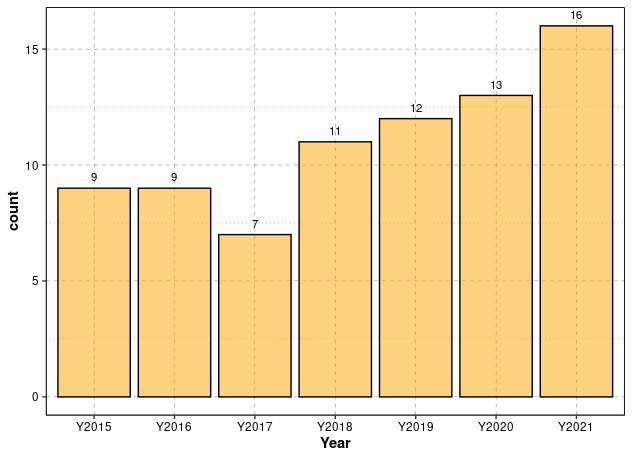
\includegraphics[width=0.6\textwidth]{análisis/numregistersyear.png}
    \caption{Número de grupos por curso académico estudiado.}
    \label{fig:groupsperyear}
\end{figure}

\section{El periodo de tiempo analizado cada año}

En el Cuadro \ref{tab:days} se muestra el número de días que dura la práctica cada año. Se puede apreciar que la duración de la práctica que estamos considerando puede variar en función del curso académico.

\begin{table}[H]
\centering
\caption{Número de días que dura la práctica cada año.}
\label{tab:days}
\begin{tabular}{cc}
\hline
\textbf{Year}  & \textbf{Length (days)}  \\ \hline
Y2015 & 32 \\
Y2016 & 23 \\
Y2017 & 29 \\
Y2018 & 17 \\
Y2019 & 27 \\
Y2020 & 16 \\
Y2021 & 38 \\ \hline
Mean & 26 \\
SD & 7.958224 \\ \hline
\end{tabular}
\end{table}

\section{El conjunto de problemas analizados cada año}

Todos los años hay $9$ problemas de dificultad similar que deben ser resueltos por todos los grupos.

Para aproximarnos al concepto subjetivo de ``dificultad del problema'' vamos a analizar el número de sesiones fallidas que necesita cada alumno para resolverlos por primera vez con respecto al número total de sesiones de ese problema (tasa de fallo) y la duración de este periodo en horas.

\subsection{Dificultad del problema: la tasa de fallo}

La apertura de un problema se corresponde con una sesión de trabajo, la cual puede terminar fracasando (fail) si no se consigue resolver el problema, o teniendo éxito (solved) en caso de que se haya resuelto el problema. Así pues, se definirá la tasa de fallo como el cociente entre el número total de sesiones fallidas y el número total de sesiones de un mismo problema. El boxplot de las tasas de fallo por problema puede verse en la Figura \ref{fig:boxplotfailratio}. En él, podemos observar que, aunque al principio cuesta empezar (la tasa de fallo del segundo problema es en media mayor que la del primero), los problemas $3$, $4$ y $5$ se resuelven con mayor facilidad y podrían considerarse equivalentes en cuanto a dificultad. Nótese, además, que la práctica está aprobada si se resuelven los cinco primeros problemas de la misma. Por otro lado, los cuatro últimos problemas presentan una dificultad creciente y superior a la de los cinco primeros problemas y determinarán la nota de la práctica. Esta tendencia primero decreciente y luego creciente se ha creado de manera intencionada por parte del profesorado para motivar al alumnado al principio de la práctica y empujarles a resolver los últimos problemas al final de la misma.

\begin{figure}[H]
    \centering
    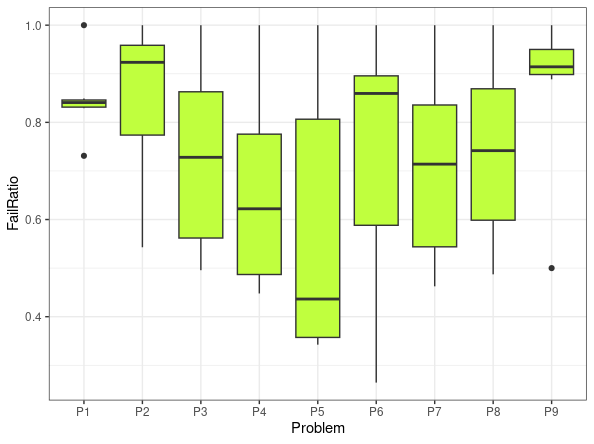
\includegraphics[width=0.8\textwidth]{análisis/boxplotfailratioproblem.png}
    \caption{Boxplot de la tasa de fallo (\emph{fail ratio}) por problema.}
    \label{fig:boxplotfailratio}
\end{figure}

Tras realizar el test ANOVA de un factor (resultados en el Cuadro \ref{tab:ANOVAfailratio}), cuya hipótesis nula establece que la tasa de fallo media de los nueve problemas considerados es la misma, se detecta que las diferencias entre las distribuciones de probabilidad de la tasa de fallo  podrían ser estadísticamente significativas en los distintos problemas ($p = 7.72e-12 < 0.05$)\footnote{Nótese que hemos establecido un nivel de significancia de $\alpha = 0.05$.}. Si aplicamos el test de Kruskal-Wallis, obtenemos $p-value = 3.756e-12 < 0.05$, lo que confirma los resultados obtenidos por el test de ANOVA.

% latex table generated in R 4.3.1 by xtable 1.8-4 package
% Wed Aug  2 16:49:26 2023
\begin{table}[H]
\centering
\caption{Resultados del test ANOVA de un solo factor (tasa de fallo).}
\label{tab:ANOVAfailratio}
\begin{tabular}{lrrrrr}
  \hline
 & Df & Sum Sq & Mean Sq & F value & Pr($>$F) \\ 
  \hline
fr & 8 & 4.00 & 0.50 & 9.12 & 7.72e-12 \\ 
  Residuals        & 570 & 31.23 & 0.05 &  &  \\ 
   \hline
\end{tabular}
\end{table}

Además, se ha realizado un test de Tukey por pares de problemas (Cuadro \ref{tab:Tukeyfailratio}). En él se observa que no todos los pares pueden considerarse estadísticamente iguales aunque haya algunos que quizá puedan serlo, como el par $P1-P2$ ($\text{p adj} = 1.00$). La Figura \ref{fig:confidenceratiofail} muestra los intervalos de confianza de todas las diferencias entre las distintas parejas de años.

\begin{table}[H]
\centering
\caption{Test HSD de Tukey (Honestly-significance-difference) de la tasa de fallo por problemas.}
\label{tab:Tukeyfailratio}
\begin{tabular}{rrrrr}
  \hline
 & diff & lwr & upr & p adj \\ 
  \hline
p2-p1 & -0.00 & -0.13 & 0.12 & 1.00 \\ 
  p3-p1 & -0.11 & -0.24 & 0.01 & 0.11 \\ 
  p4-p1 & -0.17 & -0.29 & -0.04 & 0.00 \\ 
  p5-p1 & -0.22 & -0.35 & -0.10 & 0.00 \\ 
  p6-p1 & -0.08 & -0.21 & 0.04 & 0.47 \\ 
  p7-p1 & -0.09 & -0.21 & 0.03 & 0.36 \\ 
  p8-p1 & -0.06 & -0.18 & 0.06 & 0.81 \\ 
  p9-p1 & 0.08 & -0.05 & 0.21 & 0.61 \\ 
  p3-p2 & -0.11 & -0.24 & 0.02 & 0.17 \\ 
  p4-p2 & -0.16 & -0.29 & -0.03 & 0.00 \\ 
  p5-p2 & -0.22 & -0.35 & -0.09 & 0.00 \\ 
  p6-p2 & -0.08 & -0.21 & 0.05 & 0.59 \\ 
  p7-p2 & -0.08 & -0.21 & 0.04 & 0.48 \\ 
  p8-p2 & -0.06 & -0.18 & 0.07 & 0.89 \\ 
  p9-p2 & 0.08 & -0.05 & 0.22 & 0.57 \\ 
  p4-p3 & -0.05 & -0.19 & 0.08 & 0.95 \\ 
  p5-p3 & -0.11 & -0.24 & 0.02 & 0.20 \\ 
  p6-p3 & 0.03 & -0.10 & 0.16 & 1.00 \\ 
  p7-p3 & 0.03 & -0.10 & 0.15 & 1.00 \\ 
  p8-p3 & 0.05 & -0.08 & 0.18 & 0.94 \\ 
  p9-p3 & 0.19 & 0.06 & 0.33 & 0.00 \\ 
  p5-p4 & -0.06 & -0.19 & 0.08 & 0.93 \\ 
  p6-p4 & 0.08 & -0.05 & 0.22 & 0.57 \\ 
  p7-p4 & 0.08 & -0.05 & 0.21 & 0.64 \\ 
  p8-p4 & 0.10 & -0.03 & 0.24 & 0.24 \\ 
  p9-p4 & 0.25 & 0.11 & 0.38 & 0.00 \\ 
  p6-p5 & 0.14 & 0.01 & 0.27 & 0.03 \\ 
  p7-p5 & 0.13 & 0.01 & 0.26 & 0.03 \\ 
  p8-p5 & 0.16 & 0.03 & 0.29 & 0.00 \\ 
  p9-p5 & 0.30 & 0.17 & 0.44 & 0.00 \\ 
  p7-p6 & -0.01 & -0.13 & 0.12 & 1.00 \\ 
  p8-p6 & 0.02 & -0.11 & 0.15 & 1.00 \\ 
  p9-p6 & 0.16 & 0.03 & 0.30 & 0.01 \\ 
  p8-p7 & 0.03 & -0.10 & 0.15 & 1.00 \\ 
  p9-p7 & 0.17 & 0.03 & 0.30 & 0.00 \\ 
  p9-p8 & 0.14 & 0.01 & 0.27 & 0.03 \\ 
   \hline
\end{tabular}
\end{table}

\begin{figure}[H]
    \centering
    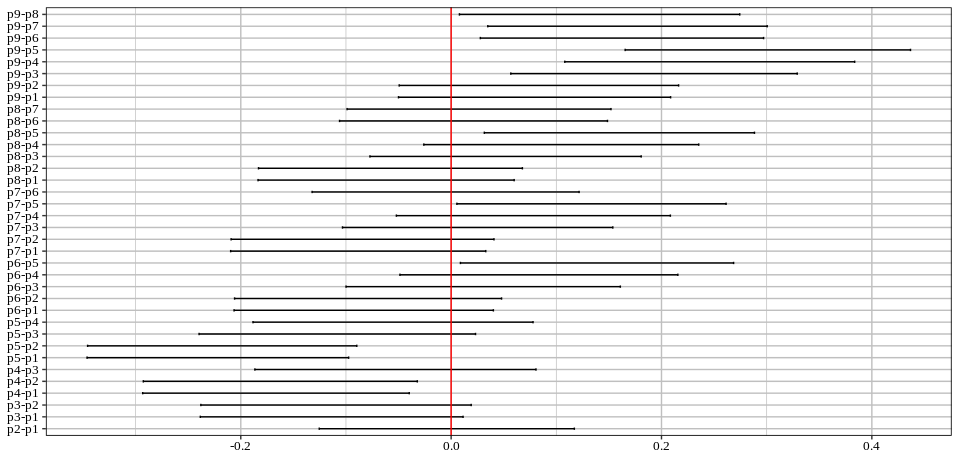
\includegraphics[width=0.80\textwidth]{análisis/confidencefailratio.png}
    \caption{Intervalos de confianza de la tasas de fallo de los problemas.}
    \label{fig:confidenceratiofail}
\end{figure}

Estos datos hay que interpretarlos de manera incremental, pues para resolver un problema $P_i$ se requieren las habilidades de los problemas $P_j$, $0\leq j < i$ más habilidades nuevas propias del problema $P_i$. Así pues, periódicamente se incrementa notablemente el nivel de dificultad. % P1 es el que más cuesta porque siempre cuesta trabajo empezar, P2-4 son muy parecidos y P5 es un poco más difícil, P6-P8 suben un escalón de dificultad y P9 también.

\subsection{Dificultad del problema: tiempo necesario en resolverlo}

Es el número de horas que transcurren desde que el problema se abre por primera vez hasta que es resuelto por primera vez. El boxplot de los tiempos de resolución por problema puede verse en la Figura \ref{fig:boxplotduration}. Así pues, en correspondencia con el boxplot de la Figura \ref{fig:boxplotfailratio}, podemos observar que los alumnos dedican más tiempo a la resolución de los problemas con una mayor tasa de fallo y, por consiguiente, más difíciles.

\begin{figure}[H]
    \centering
    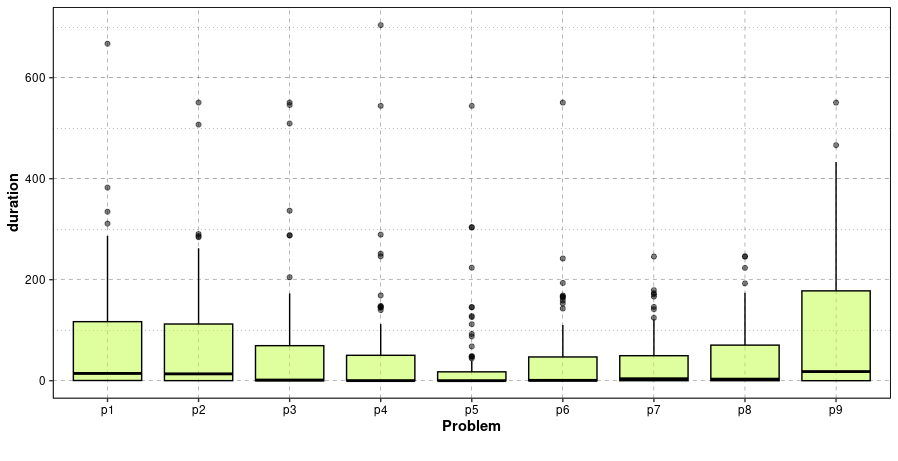
\includegraphics[width=0.8\textwidth]{análisis/boxplotduration.png}
    \caption{Boxplots del tiempo necesario para resolver cada uno de los problemas.}
    \label{fig:boxplotduration}
\end{figure}

Podemos ver un resumen del test ANOVA de un factor en el Cuadro \ref{tab:ANOVAduration}. De nuevo, los tests detectan comportamientos diferentes: obtenemos $p=0.0074$ con el test ANOVA de un solo factor y $p=0.0002763$ con la prueba de Kruskal-Wallis).

% latex table generated in R 4.3.1 by xtable 1.8-4 package
% Wed Aug  2 18:33:43 2023
\begin{table}[H]
\centering
\caption{Resultados del test ANOVA de un solo factor (tiempo en resolver los problemas por primera vez).}
\label{tab:ANOVAduration}
\begin{tabular}{lrrrrr}
  \hline
 & Df & Sum Sq & Mean Sq & F value & Pr($>$F) \\ 
  \hline
duration & 8 & 222548.19 & 27818.52 & 2.64 & 0.0074 \\ 
  Residuals           & 642 & 6757495.31 & 10525.69 &  &  \\ 
   \hline
\end{tabular}
\end{table}

Adicionalmente, se aportan los resultados del test de Tukey por pares de problemas (Cuadro \ref{tab:Tukeyduration}). En ellos se detecta, por ejemplo, que los pares de problemas $P9-P7$ y $P9-P5$ son estadísticamente diferentes ($\text{p adj} = 0.02$ en ambos casos). En la Figura \ref{fig:confidenceduration} se muestran los intervalos de confianza de todas las diferencias entre las distintas parejas de años.

% latex table generated in R 4.3.1 by xtable 1.8-4 package
% Wed Aug  2 18:34:46 2023
\begin{table}[H]
\centering
\caption{Test HSD de Tukey (Honestly-significance-difference) del tiempo de resolución por problemas.}
\label{tab:Tukeyduration}
\begin{tabular}{rrrrr}
  \hline
 & diff & lwr & upr & p adj \\ 
  \hline
p2-p1 & -8.38 & -59.84 & 43.08 & 1.00 \\ 
  p3-p1 & -14.68 & -66.66 & 37.31 & 0.99 \\ 
  p4-p1 & -22.83 & -74.99 & 29.33 & 0.91 \\ 
  p5-p1 & -41.17 & -92.97 & 10.63 & 0.25 \\ 
  p6-p1 & -34.32 & -86.85 & 18.22 & 0.52 \\ 
  p7-p1 & -41.10 & -93.26 & 11.07 & 0.26 \\ 
  p8-p1 & -27.84 & -80.38 & 24.70 & 0.78 \\ 
  p9-p1 & 19.54 & -35.45 & 74.52 & 0.97 \\ 
  p3-p2 & -6.30 & -58.28 & 45.68 & 1.00 \\ 
  p4-p2 & -14.45 & -66.61 & 37.71 & 0.99 \\ 
  p5-p2 & -32.79 & -84.60 & 19.01 & 0.56 \\ 
  p6-p2 & -25.94 & -78.48 & 26.60 & 0.84 \\ 
  p7-p2 & -32.72 & -84.88 & 19.45 & 0.58 \\ 
  p8-p2 & -19.46 & -72.00 & 33.07 & 0.97 \\ 
  p9-p2 & 27.91 & -27.07 & 82.90 & 0.82 \\ 
  p4-p3 & -8.15 & -60.83 & 44.52 & 1.00 \\ 
  p5-p3 & -26.49 & -78.81 & 25.83 & 0.82 \\ 
  p6-p3 & -19.64 & -72.69 & 33.41 & 0.97 \\ 
  p7-p3 & -26.42 & -79.10 & 26.25 & 0.83 \\ 
  p8-p3 & -13.17 & -66.21 & 39.88 & 1.00 \\ 
  p9-p3 & 34.21 & -21.26 & 89.68 & 0.60 \\ 
  p5-p4 & -18.34 & -70.84 & 34.16 & 0.98 \\ 
  p6-p4 & -11.49 & -64.71 & 41.74 & 1.00 \\ 
  p7-p4 & -18.27 & -71.12 & 34.59 & 0.98 \\ 
  p8-p4 & -5.01 & -58.24 & 48.21 & 1.00 \\ 
  p9-p4 & 42.36 & -13.28 & 98.01 & 0.30 \\ 
  p6-p5 & 6.85 & -46.02 & 59.73 & 1.00 \\ 
  p7-p5 & 0.07 & -52.43 & 52.57 & 1.00 \\ 
  p8-p5 & 13.33 & -39.55 & 66.20 & 1.00 \\ 
  p9-p5 & 60.70 & 5.40 & 116.01 & 0.02 \\ 
  p7-p6 & -6.78 & -60.00 & 46.45 & 1.00 \\ 
  p8-p6 & 6.47 & -47.12 & 60.07 & 1.00 \\ 
  p9-p6 & 53.85 & -2.14 & 109.85 & 0.07 \\ 
  p8-p7 & 13.25 & -39.97 & 66.48 & 1.00 \\ 
  p9-p7 & 60.63 & 4.99 & 116.27 & 0.02 \\ 
  p9-p8 & 47.38 & -8.62 & 103.37 & 0.17 \\ 
   \hline
\end{tabular}
\end{table}

\begin{figure}[H]
    \centering
    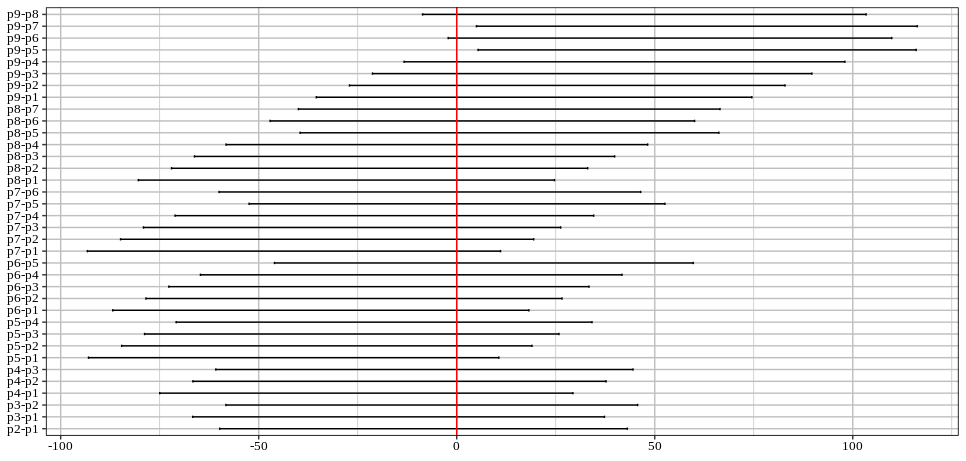
\includegraphics[width=0.80\textwidth]{análisis/confidenceduration.png}
    \caption{Intervalos de confianza del tiempo empleado en la resolución de los problemas propuestos por primera vez.}
    \label{fig:confidenceduration}
\end{figure}

Por lo tanto, se puede ver, dadas las evidencias aportadas, que la resolución de cada problema exige respuestas claramente diferentes por parte del alumnado.

\section{Actividad registrada}\label{sec:activityrecorded}

El número de registros y de sesiones de trabajo de cada uno de los años analizados se muestran en el Cuadro \ref{tab:records}. Como podemos ver, aunque el curso académico 2020-2021 (Y2020) registra más actividad que los demás, no es el que presenta el mayor número de sesiones.

\begin{table}[H]
\centering
\caption{Número de registros y sesiones almacenados en el servidor por años.}
\label{tab:records}
\begin{tabular}{ccc}
\hline
\textbf{Year}  & \textbf{Activity Records} & \textbf{Sessions}  \\ \hline
Y2015 & 12088            &  4489  \\
Y2016 & 12525            &  4538  \\
Y2017 & 9088             &  3661  \\
Y2018 & 5705             &  2811  \\
Y2019 & 14475            &  5156  \\
Y2020 & 21188            &  3904  \\
Y2021 & 11961            &  6113  \\ \hline
Mean & 12432.86 & 4381.714 \\
SD & 4789.312 & 1068.3 \\ \hline
\end{tabular}
\end{table}

Al ser un servicio $24$ horas los $7$ días de la semana, los alumnos interactúan con el laboratorio remoto en cualquier día de la semana tal y como puede verse en la Figura \ref{fig:days} y a cualquier hora del día (Figura \ref{fig:hours}). Así pues, el uso intensivo del servidor por parte del alumnado aporta solidez y fiabilidad al dataset que estamos considerando.

\begin{figure}[H]
\centering
\subfloat[Histograma de los días de la semana.]{\label{fig:days}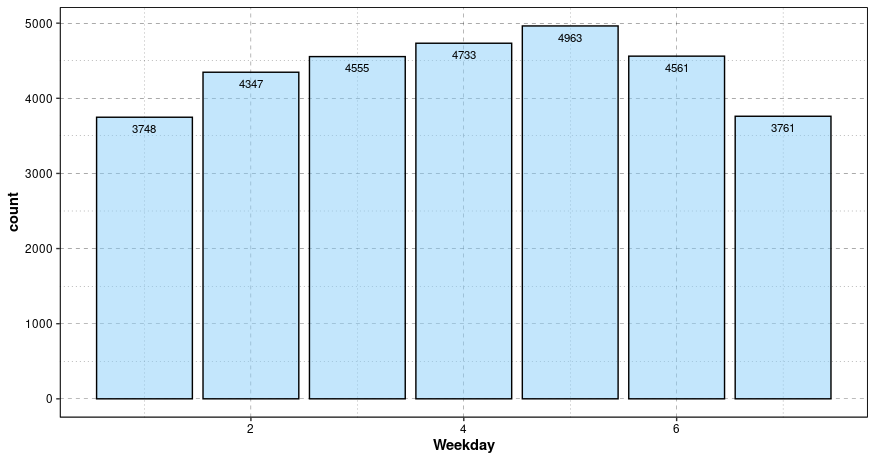
\includegraphics[width=0.9\textwidth]{análisis/days.png}}\\
\subfloat[Histograma de las horas del día.]{\label{fig:hours}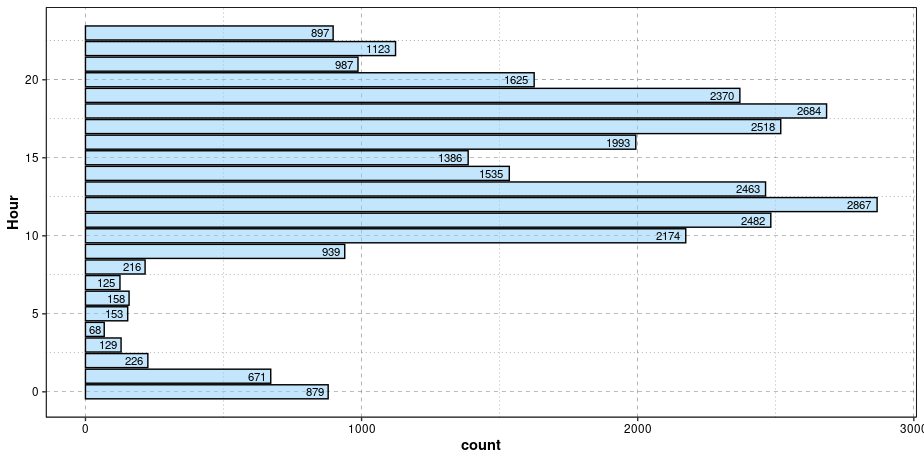
\includegraphics[width=0.9\textwidth]{análisis/hours.png}}
\caption{Actividad registrada en el servidor remoto.}
\label{fig:activity}
\end{figure}

El número y tipo de las sesiones de trabajo de cada uno de los grupos puede contemplarse en el Cuadro \ref{tab:type}.

\subsection{Análisis de la normalidad de la distribución del número de sesiones}\label{sec:NormalityNumSessions}

En las Figuras \ref{fig:boxplotresiduals} y \ref{fig:histogramresiduals} podemos ver el boxplot de los residuos de la variable número de sesiones (\emph{s}) junto con el histograma de los mismos.

\begin{figure}[H]
\centering
\subfloat[Boxplot de los residuos del número de sesiones.]{\label{fig:boxplotresiduals}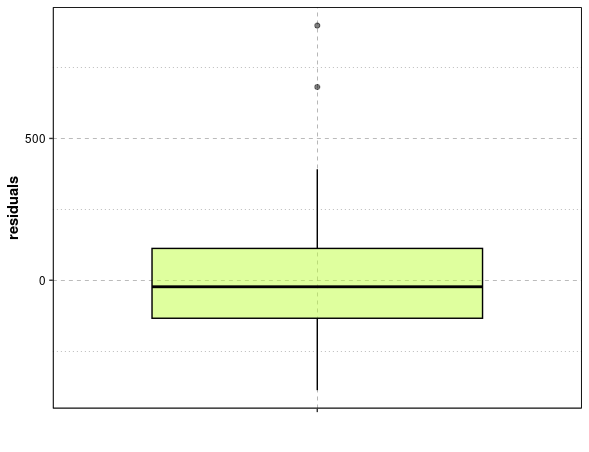
\includegraphics[width=0.47\textwidth]{análisis/residualss.png}}\qquad
\subfloat[Histograma de los residuos del número de sesiones.]{\label{fig:histogramresiduals}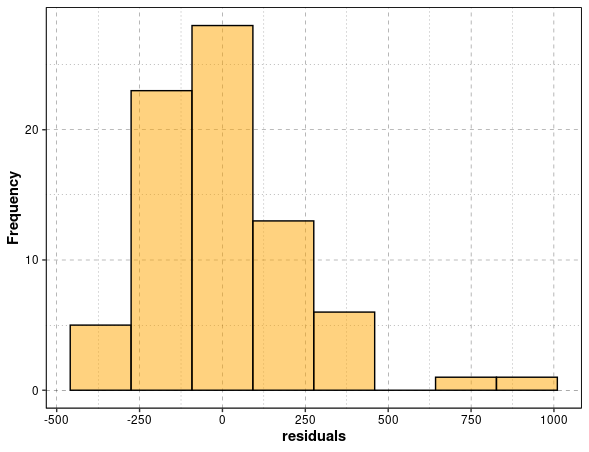
\includegraphics[width=0.47\textwidth]{análisis/histograms.png}}
\caption{Distribución de los residuos del número de sesiones.}
\label{fig:activity}
\end{figure}

A continuación, en las Figuras \ref{fig:densitysessions} y \ref{fig:q-qsessions}, podemos observar que la distribución del número de sesiones no es perfectamente normal pero es casi-normal si eliminamos algunos outsiders. La línea discontinua vertical marca el valor más probable ($336$ sesiones), lo que muestra un gran esfuerzo por parte del alumnado teniendo en cuenta la duración de la práctica (Cuadro \ref{tab:days}).

\begin{figure}[H]
    \centering
    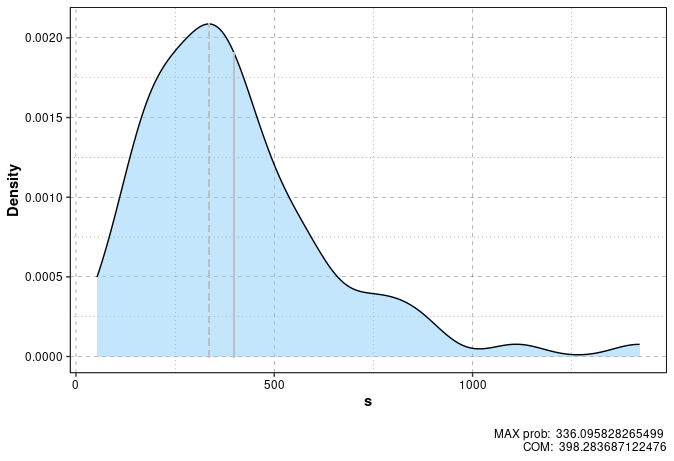
\includegraphics[width=0.70\textwidth]{análisis/densitys.png}
    \caption{Función de densidad de probabilidad del número de sesiones.}
    \label{fig:densitysessions}
\end{figure}


\begin{figure}[H]
    \centering
    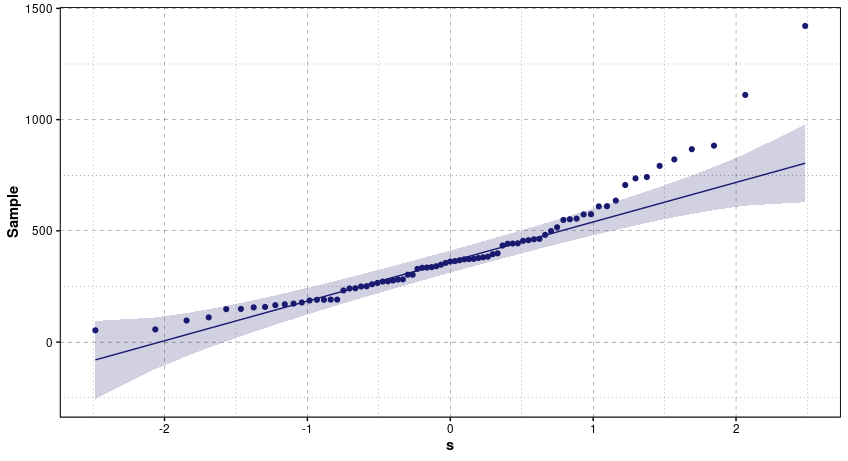
\includegraphics[width=0.75\textwidth]{análisis/qqplots.png}
    \caption{Gráfico Q-Q del número de sesiones.}
    \label{fig:q-qsessions}
\end{figure}

Además, podemos ver en la Figura \ref{fig:outlierss} que hay algunos outliers ($867$, $883$, $1421$ y $1111$) considerando la distribución del número total de sesiones por grupo de alumnos. Segmentando por años, obtenemos los boxplots que se muestran en la Figura \ref{fig:boxplotsessionsyearinitial}. Así pues, eliminaremos aquellos registros que sean outliers en todos los años. Tras realizar la acción anterior, obtenemos la distribución del número de sesiones que se muestra en la Figura \ref{fig:outlierss2}.

\begin{figure}[H]
    \centering
    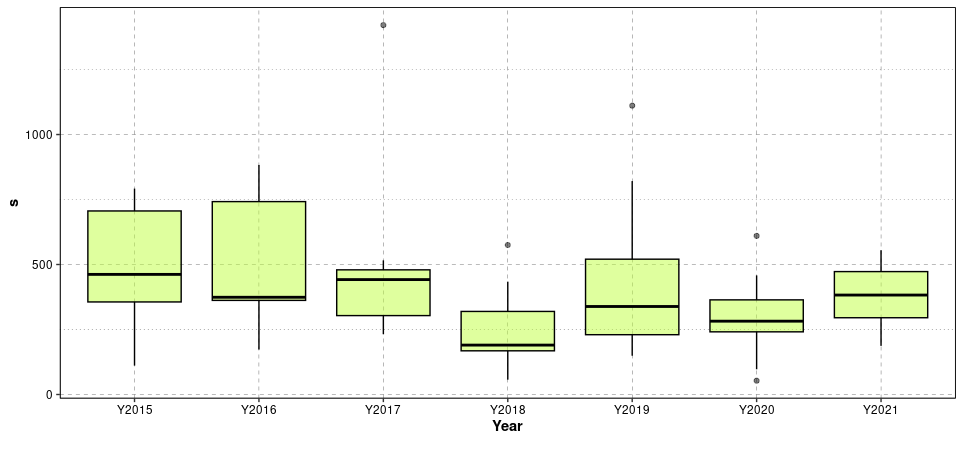
\includegraphics[width=0.80\textwidth]{análisis/boxplotinitials.png}
    \caption{Boxplot del número de sesiones por año inicialmente.}
    \label{fig:boxplotsessionsyearinitial}
\end{figure}

\begin{figure}[H]
    \centering
    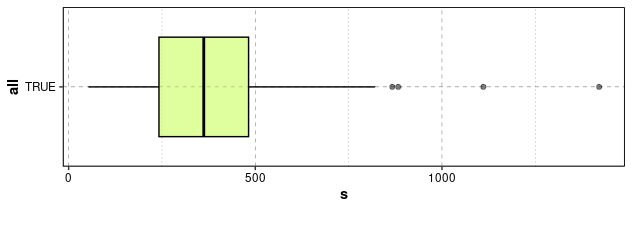
\includegraphics[width=0.60\textwidth]{análisis/outlierss.png}
    \caption{Distribución del número de sesiones inicial.}
    \label{fig:outlierss}
\end{figure}

\begin{figure}[H]
    \centering
    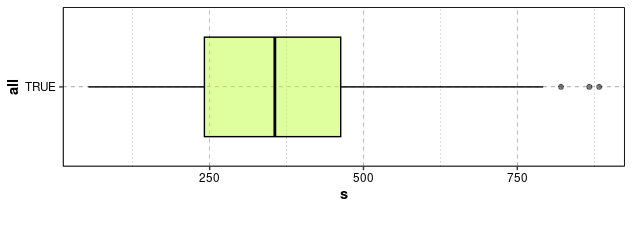
\includegraphics[width=0.60\textwidth]{análisis/outlierss2.png}
    \caption{Distribución del número de sesiones tras la eliminación de algunos outliers.}
    \label{fig:outlierss2}
\end{figure}

Examinamos ahora los bloques significativos entre ellos agrupando los datos en ocho particiones mediante el algoritmo de las K-medias, tal y como se muestra en la Figura \ref{fig:KMeans8}. Los resultados obtenidos pueden verse en las Figuras \ref{fig:KMeans8boxplot} y \ref{fig:KMeans8count}.

\begin{figure}[H]
    \centering
    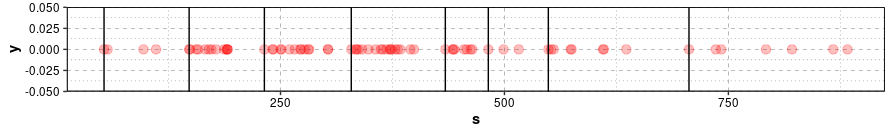
\includegraphics[width=0.6\textwidth]{análisis/KMeanss8.png}
    \caption{Particiones obtenidas con $K = 8$.}
    \label{fig:KMeans8}
\end{figure}

\begin{figure}[H]
\centering
\subfloat[Boxplot de cada una de las particiones.]{\label{fig:KMeans8boxplot}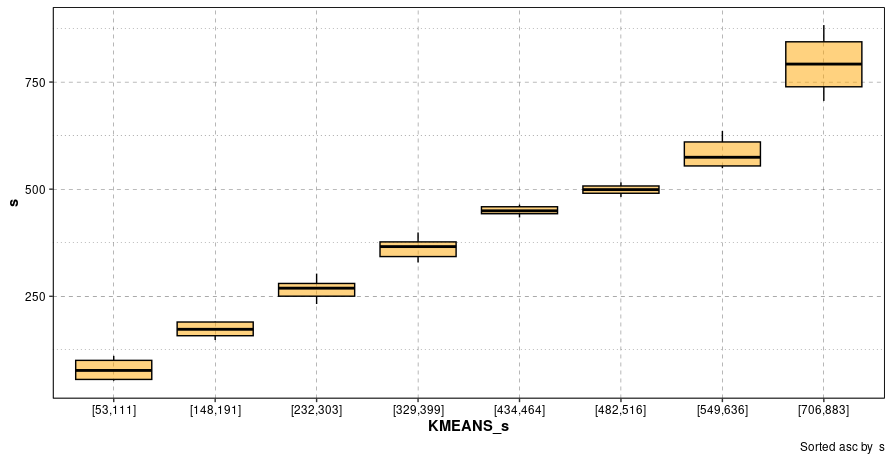
\includegraphics[width=0.47\textwidth]{análisis/KMeanssboxplot.png}}\qquad
\subfloat[Número de grupos por partición.]{\label{fig:KMeans8count}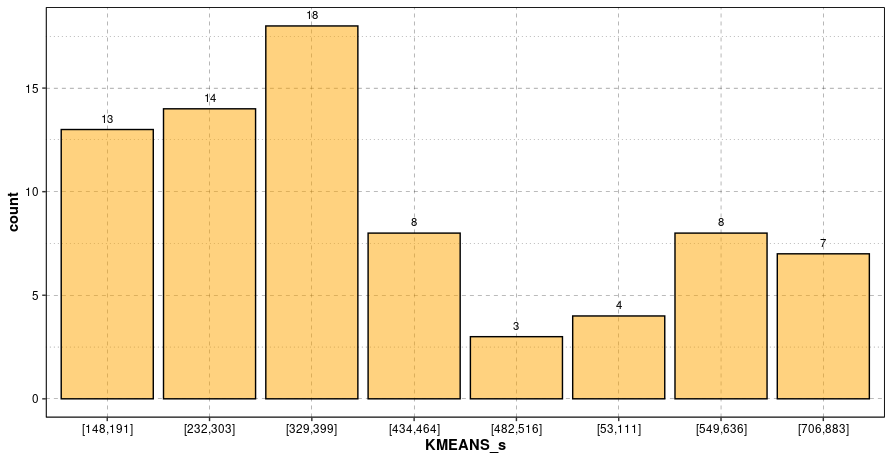
\includegraphics[width=0.47\textwidth]{análisis/KMeansscount.png}}%
\caption{Resultados obtenidos tras aplicar el algoritmo de las $K$-Medias con $K = 8$.}
\label{fig:KMeans8details}
\end{figure}

Nótese que como hemos una obtenido una precisión del $97.95579\% > 95\%$, no eliminaremos más outliers.

Así pues, tras la eliminación de los outliers correspondientes tanto al número de sesiones como al número de problemas resueltos como veremos en la subsección \ref{sec:NumProblems} (podemos ver la nueva función de densidad en la Figura \ref{fig:normalitys}) se procede a aplicar el test de normalidad de Shapiro-Wilk. Como se obtiene $p-value = 0.003307 < 0.05$, podemos decir que estadísticamente no sigue una distribución normal. No obstante, teniendo en cuenta que el tamaño de la muestra es relativamente pequeño (tenemos un total de $77$ grupos de prácticas), podemos considerar que se trata de una distribución normal.

\begin{figure}[H]
    \centering
    \includegraphics[width=0.70\textwidth]{análisis/normalitys.png}
    \caption{Función de densidad de probabilidad del número de sesiones tras eliminar algunos outliers.}
    \label{fig:normalitys}
\end{figure}

\subsection{Sesiones por cada problema}

En la Figura \ref{fig:boxplotsessionsproblem} podemos ver el boxplot del número de sesiones por problema. Como podemos ver, el problema P1 es mucho más frecuentado que el resto. No obstante, la diferencia entre el número de sesiones abiertas del problema P1 y el número de sesiones abiertas de los problemas restantes se debe a que los alumnos utilizan el primer problema como base de todos los experimentos y para testear las comunicaciones con el servidor. Así pues, el problema P1 es frecuentemente utilizado, no ya sólo al comienzo de la práctica, sino durante todo el desarrollo de la misma.

\begin{figure}[H]
    \centering
    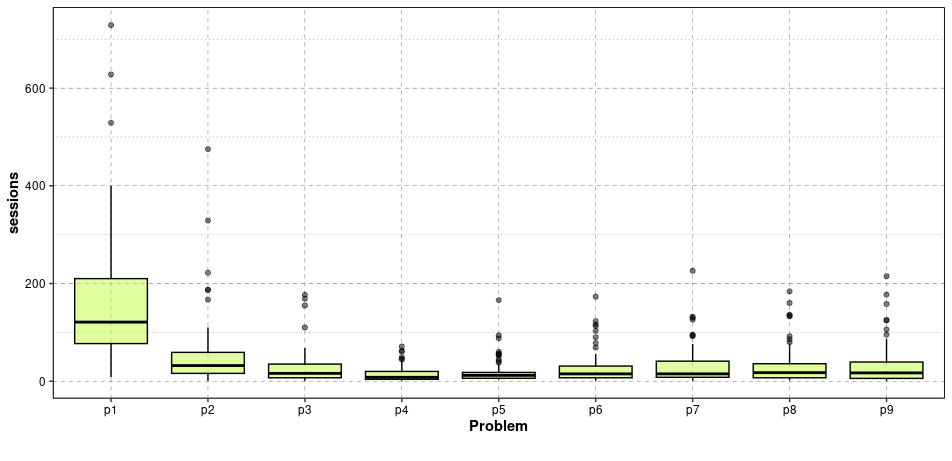
\includegraphics[width=0.8\textwidth]{análisis/boxplotsessionsproblem.png}
    \caption{Boxplot del número de sesiones por problema.}
    \label{fig:boxplotsessionsproblem}
\end{figure}

\subsection{Sesiones cada año}\label{sec:ANOVANumSessions}

Como podemos ver en la Figura \ref{fig:boxplotsessionsyear}, las sesiones de trabajo abiertas en el servidor año tras año, parecen seguir la misma distribución de probabilidad.

\begin{figure}[H]
    \centering
    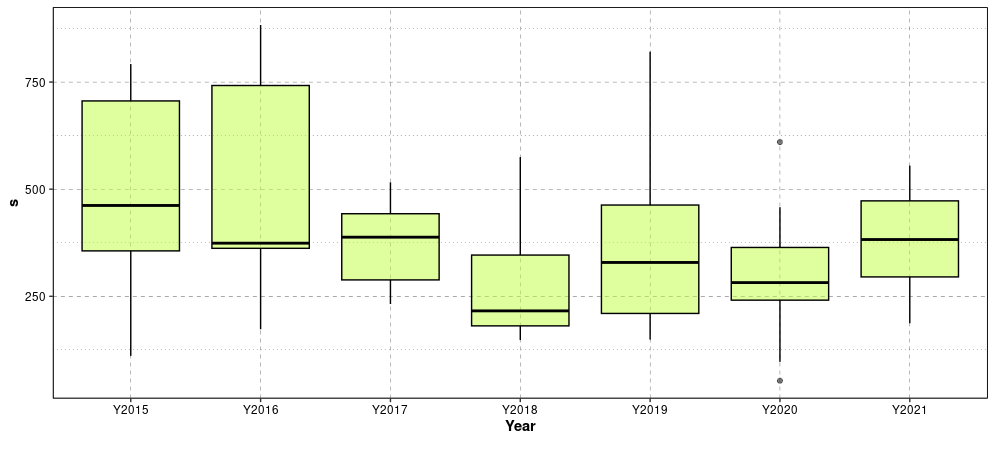
\includegraphics[width=0.80\textwidth]{análisis/boxplotfinals.png}
    \caption{Boxplot del número de sesiones por año tras la eliminación de algunos outliers.}
    \label{fig:boxplotsessionsyear}
\end{figure}

Un resumen de los resultados obtenidos al realizar el test ANOVA se muestra en el Cuadro \ref{tab:ANOVAnumsessions}. La hipótesis nula establece que el número de sesiones medio de los siete cursos académicos estudiados es el mismo. Así pues, estableciendo un nivel de significancia de $0.05$, como tenemos que $p = 0.0412 < 0.05$, por lo que las diferencias entre las medias podrían ser estadísticamente significativas. Aplicando el test de Kruskal-Wallis, obtenemos un $p-value$ igual a $0.08798 > 0.05$.

% latex table generated in R 4.3.0 by xtable 1.8-4 package
% Sat May 27 18:26:28 2023
\begin{table}[H]
\centering
\caption{Resultados del test ANOVA de un solo factor (número de sesiones).}
\label{tab:ANOVAnumsessions}
\begin{tabular}{lrrrrr}
  \hline
 & Df & Sum Sq & Mean Sq & F value & Pr($>$F) \\ 
  \hline
s & 6 & 460434.32 & 76739.05 & 2.34 & 0.0412 \\ 
  Residuals         & 67 & 2197451.96 & 32797.79 &  &  \\ 
   \hline
\end{tabular}
\end{table}

Además, se ha realizado un test de Tukey por pares de años (Cuadro \ref{tab:Tukeynumsessions}). En él se observa que todos los pares pueden considerarse estadísticamente iguales ($\text{p adj} > 0.1$ en todos ellos). Así pues, podemos concluir que el número de sesiones abiertas en el servidor sigue la misma distribución de probabilidad año tras año.

La Figura \ref{fig:confidencenumsessions} muestra los intervalos de confianza de todas las diferencias entre las distintas parejas de años. Así pues, consideraremos que el número de sesiones de cada grupo por año es equivalente (las variaciones son debidas al azar). Esto es importante porque indica que el comportamiento más básico de los alumnos, que viene dado por cuántas veces se conectan al servidor, es el mismo en todos los cursos académicos considerados.

% latex table generated in R 4.3.0 by xtable 1.8-4 package
% Sat May 27 18:26:44 2023
\begin{table}[H]
\centering
\caption{Test HSD de Tukey (Honestly-significance-difference) del número de sesiones por años.}
\label{tab:Tukeynumsessions}
\begin{tabular}{rrrrr}
  \hline
 & diff & lwr & upr & p adj \\ 
  \hline
Y2016-Y2015 & 5.44 & -254.06 & 264.95 & 1.00 \\ 
  Y2017-Y2015 & -125.44 & -415.58 & 164.69 & 0.84 \\ 
  Y2018-Y2015 & -223.38 & -476.31 & 29.56 & 0.12 \\ 
  Y2019-Y2015 & -131.05 & -378.48 & 116.38 & 0.68 \\ 
  Y2020-Y2015 & -198.78 & -437.49 & 39.93 & 0.16 \\ 
  Y2021-Y2015 & -116.72 & -346.09 & 112.66 & 0.72 \\ 
  Y2017-Y2016 & -130.89 & -421.03 & 159.25 & 0.81 \\ 
  Y2018-Y2016 & -228.82 & -481.76 & 24.11 & 0.10 \\ 
  Y2019-Y2016 & -136.49 & -383.92 & 110.93 & 0.63 \\ 
  Y2020-Y2016 & -204.22 & -442.93 & 34.49 & 0.14 \\ 
  Y2021-Y2016 & -122.16 & -351.53 & 107.21 & 0.67 \\ 
  Y2018-Y2017 & -97.93 & -382.21 & 186.34 & 0.94 \\ 
  Y2019-Y2017 & -5.61 & -284.99 & 273.78 & 1.00 \\ 
  Y2020-Y2017 & -73.33 & -345.03 & 198.36 & 0.98 \\ 
  Y2021-Y2017 & 8.73 & -254.80 & 272.26 & 1.00 \\ 
  Y2019-Y2018 & 92.33 & -148.20 & 332.86 & 0.90 \\ 
  Y2020-Y2018 & 24.60 & -206.95 & 256.15 & 1.00 \\ 
  Y2021-Y2018 & 106.66 & -115.25 & 328.57 & 0.77 \\ 
  Y2020-Y2019 & -67.73 & -293.25 & 157.80 & 0.97 \\ 
  Y2021-Y2019 & 14.34 & -201.28 & 229.95 & 1.00 \\ 
  Y2021-Y2020 & 82.06 & -123.49 & 287.61 & 0.89 \\ 
   \hline
\end{tabular}
\end{table}

\begin{figure}[H]
    \centering
    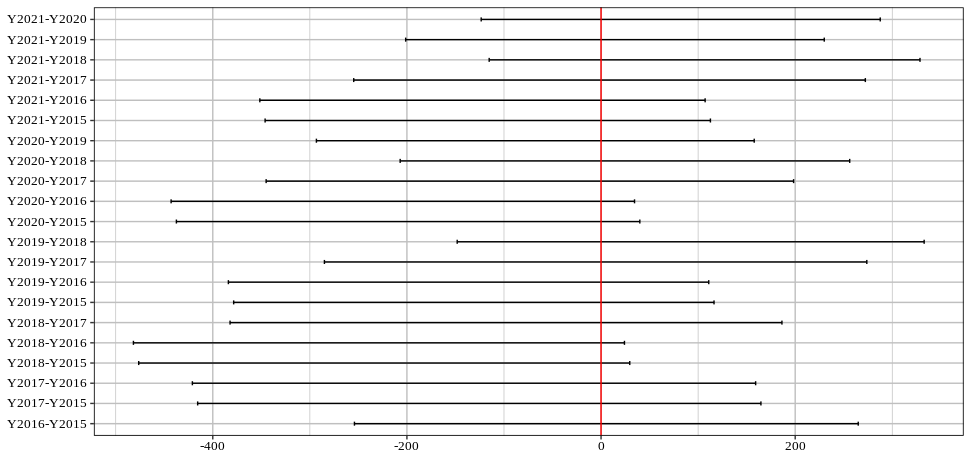
\includegraphics[width=0.80\textwidth]{análisis/confidences.png}
    \caption{Intervalos de confianza del número de sesiones por años.}
    \label{fig:confidencenumsessions}
\end{figure}

\subsection{Análisis de la distribución del número de problemas resueltos}\label{sec:NumProblems}

Además, a partir de los registros almacenados en el servidor se calcularán el número de problemas resueltos por cada grupo de prácticas. Como se puede intuir, se tratará de una variable discreta. En la Figura \ref{fig:initialp} podemos ver que el número de problemas resueltos oscila entre $6$ y $9$.

\begin{figure}[H]
    \centering
    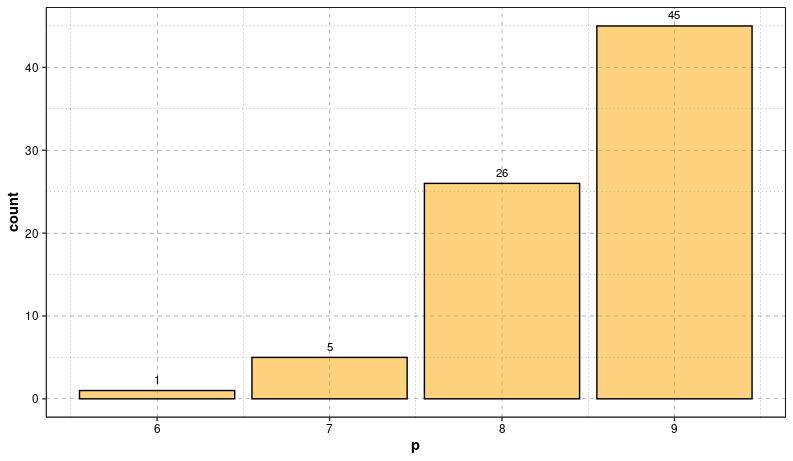
\includegraphics[width=0.6\textwidth]{rendimiento/initialp.png}
    \caption{Distribución del número de problemas resueltos.}
    \label{fig:initialp}
\end{figure}

Adicionalmente, podemos observar en la Figura \ref{fig:outliersp} la existencia de un elemento extremo ($6$) en la distribución del número de problemas resueltos por grupo de alumnos. Segmentando por años, obtenemos los boxplots que se muestran en la Figura \ref{fig:boxplotproblemsyear}. Así pues, eliminaremos el outlier encontrado puesto que se trata de un valor extremo en todos los años incluidos en este estudio.

\begin{figure}[H]
    \centering
    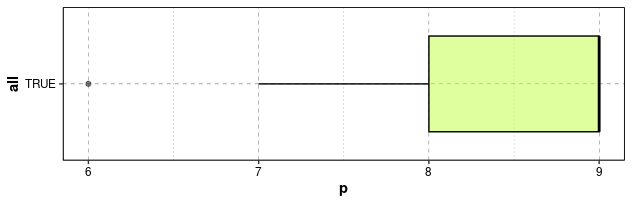
\includegraphics[width=0.60\textwidth]{análisis/outliersp.png}
    \caption{Distribución del número de problemas resueltos inicial.}
    \label{fig:outliersp}
\end{figure}

\begin{figure}[H]
    \centering
    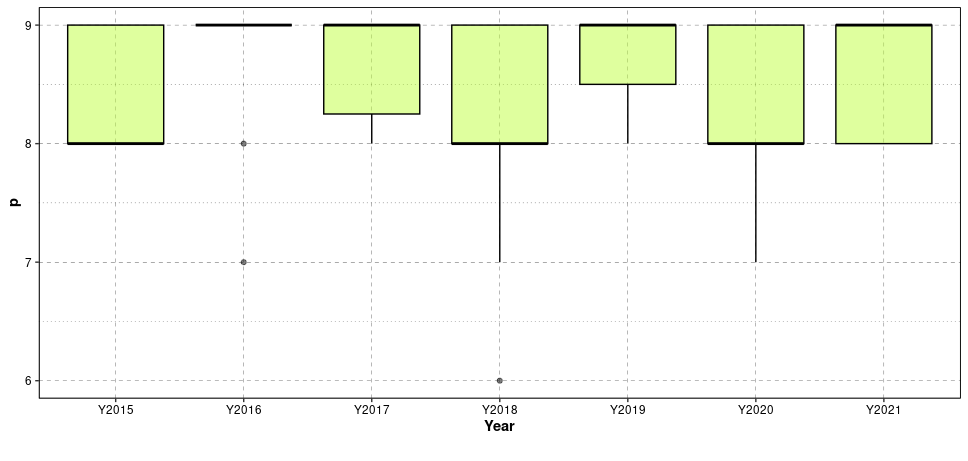
\includegraphics[width=0.80\textwidth]{análisis/boxplotinitialp.png}
    \caption{Boxplot del número de problemas resueltos por año.}
    \label{fig:boxplotproblemsyear}
\end{figure}
\chapter{Hipótesis de estudio}
\addcontentsline{toc}{chapter}{Hipótesis de estudio}

A pesar de que el estudio descriptivo anterior muestra unos datos muy variados, casi todos ellos son homogéneos año tras año. No obstante, el objetivo de este estudio es sentar las bases para conseguir una experiencia de aprendizaje óptima para todos los grupos de alumnos. Así pues, se va a poner énfasis en detectar a aquellos grupos que estén en riesgo de obtener un peor rendimiento o peores calificaciones. La detección temprana de éstos podría permitir al profesor actuar a tiempo para mejorar su proceso de aprendizaje. Para ello, se van a proponer una serie de métricas de calidad que se definirán sobre los registros de actividad de los alumnos con el objetivo de encontrar aquella que, con mayor certeza, identifique a los alumnos que peor están progresando.

\section{Métricas de calidad y correlaciones entre ellas}

Se definirán dos grandes grupos de métricas. El primer grupo consistirá en una colección de métricas de los grupos que solamente podrán calcularse tras la finalización de la práctica. Por el contrario, las métricas del segundo grupo podrán calcularse durante la realización de la práctica y, por tanto, serán más interesantes porque podrán facilitar la detección precoz de los grupos en riesgo.

Gráficamente, las medidas se han representado en la Figura \ref{fig:measures}.

\begin{figure}[H]
    \centering
    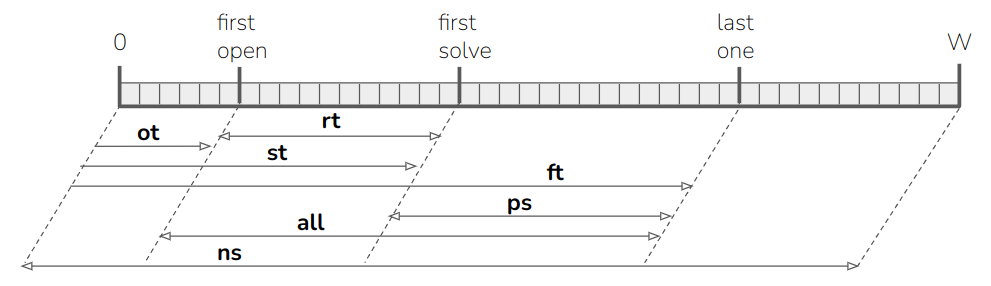
\includegraphics[width=\textwidth]{hipótesis/measures.png}
    \caption{Representación gráfica de las medidas de rendimiento empleadas que se extraen directamente de los registros del servidor (no se incluyen las medidas derivadas del análisis espectral de grafos).}
    \label{fig:measures}
\end{figure}

\subsection{Medidas a posteriori del resultado de la práctica}

\begin{itemize}
\item La calificación conseguida por el alumno (\emph{Grade}). Obviamente, cuanto mayor sea ésta, mejor.
\item Número de problemas resueltos u objetivos resueltos. Se denotará por \emph{p}. Trivialmente, cuantos más objetivos haya resuelto un grupo, mejor. El número de problemas normalizado se denotará por \emph{np} en los estudios que se realizarán a continuación.
\item Punto de finalización de toda la práctica. En la Figura \ref{fig:measures}  se representa esta medida de rendimiento normalizada por \emph{ft}. Cuanto antes, mejor (para disponer de más tiempo para repasar y corregir errores). Sin embargo, no es una métrica muy relevante.
\item Tiempo consumido por el alumno durante las prácticas. Este es un valor trampa, pues puede significar algo positivo (el alumno ha tardado poco en resolver la práctica porque la domina), o negativo (porque no ha podido dedicarle más tiempo). En la Figura \ref{fig:measures}, el tiempo consumido normalizado se representa por \emph{all}.
\item Número de sesiones realizadas (\emph{s}). Ya se ha hecho un estudio de esta medida en la sección \ref{sec:activityrecorded}. En la Figura \ref{fig:measures}, se representa el número de sesiones normalizado (\emph{ns}).
\end{itemize}

\subsection{Medidas continuas durante la práctica}

\begin{itemize}
\item Como los comienzos son siempre costosos, se definirá una nueva métrica correspondiente al promedio de tiempo de la primera apertura de cada problema. Se representa por \emph{ot} en la Figura \ref{fig:measures}.
\item Número de fails consecutivos (\emph{fail ratio} o \emph{fr}) hasta resolver un problema dividido entre el numero de sesiones de ese problema. La tasa de fallo así como el tiempo dedicado a un mismo problema dependerá de la dificultad del mismo.
%\item \emph{También se definirá una medida que cuantificará la posposición de tareas de los grupos. Es decir, pretende identificar a aquellos alumnos que, cuando intentan resolver un problema y no lo consiguen, saltan, curiosamente, a otros problemas más complejos (los cuales, obviamente, tampoco pueden resolver) perdiendo así un tiempo precioso.}
\item Tiempo promedio empleado en resolver los problemas (representado por \emph{rt}).
\item Tiempo promedio empleado en los problemas tras su resolución. Se representa por \emph{ps} en la Figura \ref{fig:measures} y trata de evidenciar el interés de los alumnos en la materia. En general, será positivo que los grupos no sólo resuelvan los problemas sino que traten de encontrar mejores soluciones para los mismos como se podrá ver en el Capítulo \ref{chapter:correlations}.
\item Tiempo de promedio de resolución de los problemas por primera vez. Se representará por \emph{st} en la Figura \ref{fig:measures}.
\item Se tendrá igualmente una medida que refleja si los grupos de prácticas siguen el orden esperado de las mismas. Se le denotará por \emph{sq} en los análisis que se realizarán posteriormente.
\item El coeficiente \emph{DAG}, que cuantificará como de balanceado están los grafos que describen la actividad de un grupo en la plataforma. Se trata una medida de rendimiento basada en el análisis espectral de grafos que se verá más adelante.
\item El coeficiente de \emph{Laplace}.
\end{itemize}
\subsection{Abrir un problema por primera vez (Newcomer)}

Momento exacto en el que se consigue abrir cada problema por primera vez en el servidor, normalizado para poder compararlo (normalizado porque cada año ha durado  un tiempo diferente)

\subsection{Resolver un problema por primera vez (EarlyBird)}

Momento exacto en el que se consigue resolver cada problema por primera vez, normalizado para poder compararlo (normalizado porque cada año ha durado  un tiempo diferente)

\textbf{Falta boxplot.}

Parece que, aunque los problemas están ordenados en orden creciente de dificultad, no siempre se resuelven en el mismo orden que se espera (ANOVA p=6.01e-7, KW p=1.18e-6), es decir P1 P2 P3 P4 P5 P6 P7 P8 P9. De hecho, se ha analizado este patrón y se han encontrado las siguientes variaciones en el que la más frecuente es la esperada por el profesor.

\subsection{Siguiendo el plan del profesor (Follower)}

Se incorpora una medida de similaridad Follower en [0,1] que cuantifica cómo se parece el patrón encontrado con respecto al patrón esperado. \textbf{Falta footnote.}

\textbf{Falta tabla.}

\ctparttext{
  \color{black}
  \begin{center}
    Estructuración en objetivos, división en sprints y seguimiento.
  \end{center}
}
\part{Planificación del proyecto}\label{sec:parteIV}

\chapter{Etapas del proyecto: división en objetivos}\label{chapter:objetivos}
\addcontentsline{toc}{chapter}{Etapas del proyecto: división en objetivos}

El proyecto se ha realizado siguiendo la metodología \emph{Scrum}
Durante la fase inicial de planificación del proyecto se realizó una subdivisión del mismo en iteraciones:
\begin{itemize}
\item Realización de un estudio multianual y segmentado por calificaciones y primeros resultados de homogeneidad de las muestras transversal por años mediante la realición de análisis ANOVA.
\item Extracción de procesos ocultos en los datasets utilizando el programa DISCO y programación y mejora del proceso de extracción. El resultado de esta fase serán una serie de grafos representando a cada uno de los grupos de prácticas considerados donde los arcos implican una relación de dependencia temporal. Estos grafos se representarán a partir de matrices de adyacencia cuyos vértices podrán representar problemas de prácticas, pares problema de prácticas y milestone alcanzado o pares problema de prácticas y estado (\texttt{FAIL} si no se ha resuelto el problema y \texttt{OK} en caso contrario).
\item Análisis de los procesos por distintas categorías: por años (resultando ser estadísticamente iguales) y por calificación final del grupo (resultando en la existencia de diferencias). Así pues, se pretenderá caracterizar el comportamiento de los grupos.
\item Análisis del comportamiento de un mismo grupo a lo largo del tiempo. Se realizará un estudio con el fin de determinar si el comportamiento de un grupo varía durante el desarrollo de las prácticas.
\end{itemize}
\chapter{Etapas del proyecto: división en sprints y seguimiento de los mismos}\label{chapter:sprints}
\addcontentsline{toc}{chapter}{Etapas del proyecto: división en sprints}

El proyecto se ha dividido en once sprints de tres semanas cada uno y un último sprint con los días restantes. Además, durante el transcurso de cada sprint se ha realizado un seguimiento del trabajo realizado en el mismo, aportando \emph{burndown charts} de cada uno de ellos.

Un \emph{burdown chart} es una gráfica en la que se muestra el progreso de un proyecto durante cierto periodo de tiempo preestablecido (un sprint, una release o el proyecto completo, por ejemplo). Para la construcción de los mismos se requieren los siguientes elementos:
\begin{itemize}
\item El periodo de \emph{tiempo a analizar}, que se corresponderá con el eje X de la gráfica. El inicio del periodo temporal vendrá representado por $x = 0$ mientras que el final de dicho periodo será representado por $x = t$ donde $t$ es la duración del periodo. Si observamos el burndown chart global del proyecto (Figura global), estos dos valores se corresponderán, respectivamente, con las fechas de inicio y finalización del mismo.
\item La cantidad de trabajo a realizar, que se corresponderá con el eje Y de la gráfica y representa el trabajo planificado que se deberá realizar en el periodo de tiempo a analizar. Cuando se realiza la estimación de las tareas, independientemente de la unidad de estimación empleada, se obtiene una cantidad de trabajo a realizar (en horas, por ejemplo). Así pues, la cantidad de trabajo restante irá decreciendo conforme el tiempo vaya avanzando.
\item Una referencia ideal, que será la línea diagonal trazada desde la esquina superior izquierda hasta la esquina inferior derecha de la gráfica. Se trata de una representación de la relación ideal entre la disminución de la cantidad de trabajo y el tiempo dedicado durante el transcurso de la fase correspondiente. Esto es, cuanto más se aproxime la línea real a la ideal se estará trabajando de mejor manera en relación a la consecución de los objetivos marcados.
\end{itemize}

Adicionalmente, si se poseen conocimientos y experiencia trabajando con herramientas ágiles, se puede obtener información útil en ellas sobre el seguimiento del proyecto con el fin de impulsar buenas prácticas y mejorar el desarrollo del mismo.

\section{Análisis de cada sprint}

\begin{figure}[H]
\centering
\subfloat[Burndown chart del sprint 1 (periodo del 12/12/2022 al 01/01/2023).]{\label{fig:sprint1}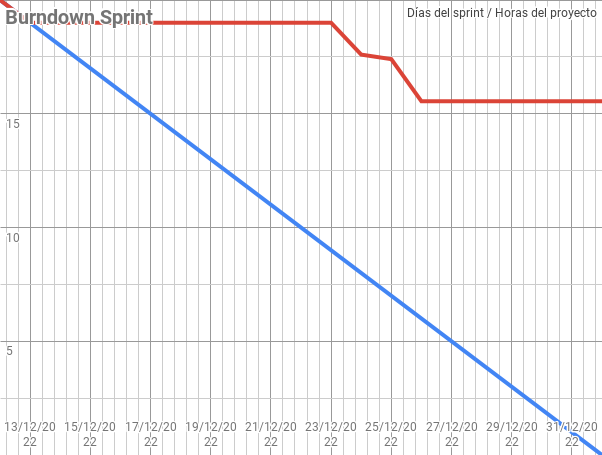
\includegraphics[width=0.46\textwidth]{sprints/Burndown Sprint 1.png}}\qquad
\subfloat[Burndown chart del sprint 2 (periodo del 02/01/2023 al 22/01/2023).]{\label{fig:sprint2}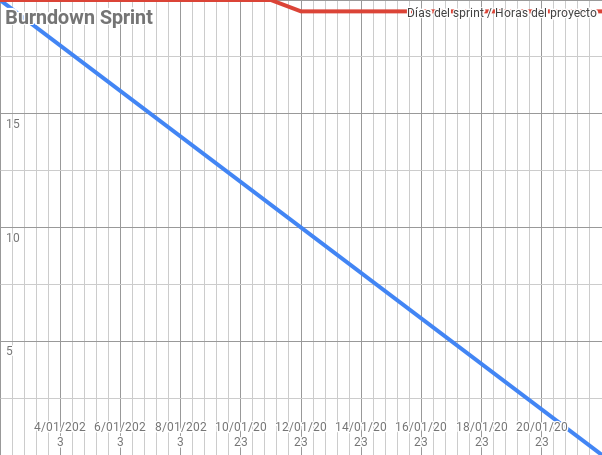
\includegraphics[width=0.46\textwidth]{sprints/Burndown Sprint 2.png}}\qquad
\subfloat[Burndown chart del sprint 3 (periodo del 23/01/2023 al 12/02/2023).]{\label{fig:sprint3}
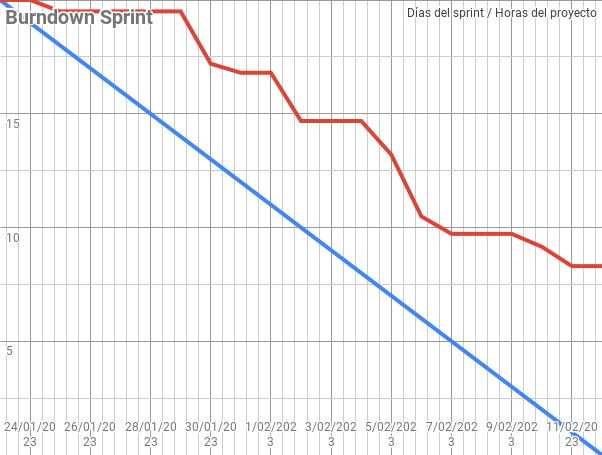
\includegraphics[width=0.46\textwidth]{sprints/Burndown Sprint 3.png}}\qquad
\subfloat[Burndown chart del sprint 4 (periodo del 13/02/2023 al 05/03/2023).]{\label{fig:sprint4}
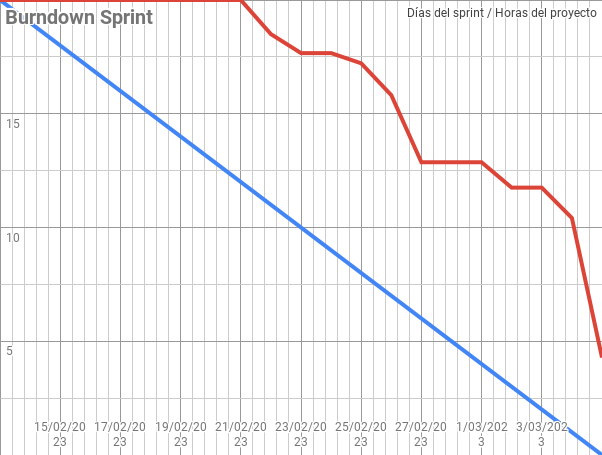
\includegraphics[width=0.46\textwidth]{sprints/Burndown Sprint 4.png}}\qquad
\subfloat[Burndown chart del sprint 5 (periodo del 06/03/2023 al 26/03/2023).]{\label{fig:sprint5}
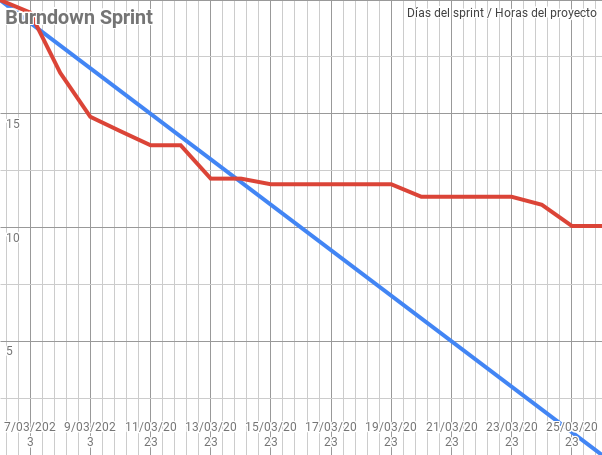
\includegraphics[width=0.46\textwidth]{sprints/Burndown Sprint 5.png}}\qquad
\subfloat[Burndown chart del sprint 6 (periodo del 27/03/2023 al 16/04/2023).]{\label{fig:sprint6}
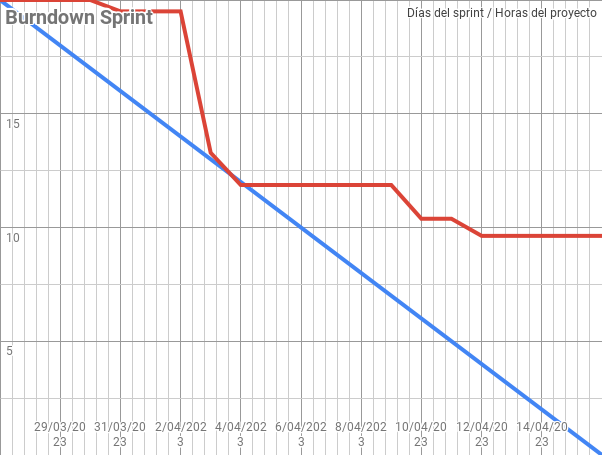
\includegraphics[width=0.46\textwidth]{sprints/Burndown Sprint 6.png}}
\caption{Burdown charts de los seis primeros sprints del proyecto.}
\label{fig:sprints1-6}
\end{figure}

\subsection{Sprint 1 (Figura \ref{fig:sprint1})}

Este primer sprint representa una situación anómala que no se debería dar. La explicación es sencilla: las líneas rojas horizontales representan periodos de tiempo en los cuales no se ha estado trabajando en el proyecto. No obstante, esto es correcto puesto que aunque se definieron unos objetivos al principio, todavía no tenía claro el procedimiento a seguir para la consecución de los mismos. Aunque podría haberse omitido este periodo de seguimiento, se ha decidio incluirlo como muestra de una tendencia no deseable en relación al desarrollo de un proyecto.

\subsection{Sprint 2 (Figura \ref{fig:sprint2})}

En este segundo sprint tampoco se han alcanzado los objetivos de trabajo preestablecidos. No obstante, es correcto porque este periodo coincide con la realización de exámenes y se planificó previamente para el estudio de los mismos y no para continuar con la realización de este trabajo fin de grado. Como se ha comentado anteriormente, durante el desarrollo de un proyecto, esta situación no debería ocurrir bajo ninguna circunstancia.

\subsection{Sprint 3 (Figura \ref{fig:sprint3})}

En este caso, la Figura \ref{fig:sprint3} muestra que se realizó una gran cantidad de trabajo focalizada en días concretos distribuidos a lo largo de todo el sprint con algunos parones entre medias. Sin embargo, a pesar de todo, no se consiguió llegar a la cantidad estipulada de trabajo al final del sprint.

\subsection{Sprint 4 (Figura \ref{fig:sprint4})}

Este cuarto sprint consiste en un periodo inicial inactivo seguido de varios picos de productividad en días concretos del sprint. Finalmente, podemos observar que se realizó una gran cantidad de trabajo al final del sprint, quedándose muy cerca la cantidad de trabajo realizada de la referencia ideal.

\subsection{Sprint 5 (Figura \ref{fig:sprint5})}

En este sprint podemos ver que se realizó más trabajo del requerido durante el primer tercio del mismo. Sin embargo, a partir de entonces, a pesar de que se avanza en días concretos, el ritmo de trabajo es mucho más lento y se termina por no realizar la cantidad de trabajo planificado durante dicho periodo temporal.

\subsection{Sprint 6 (Figura \ref{fig:sprint6})}

La gráfica de este sprint (Figura \ref{fig:sprint6}) muestra que se realizó una gran cantidad de trabajo al principio del sprint llegando la curva de trabajo real a cortar a la curva ideal un poco antes de la mitad de la misma. No obstante, al final del sprint hubo algún día de parón y el ritmo de trabajo se redujo. En consecuencia, no se alcanzaron los objetivos preestablecidos.

\begin{figure}[H]
\centering
\subfloat[Burndown chart del sprint 7 (periodo del 17/04/2023 al 07/05/2023).]{\label{fig:sprint7}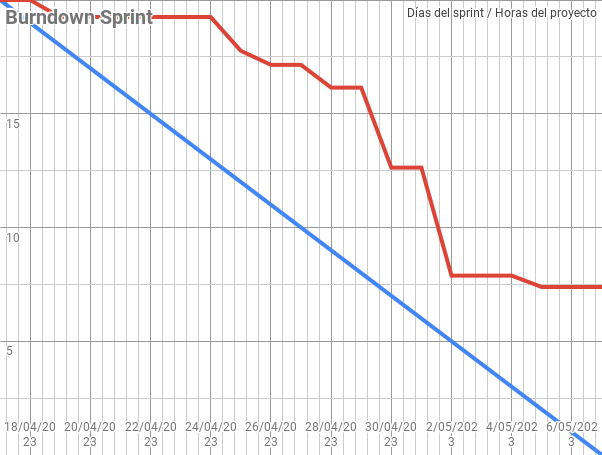
\includegraphics[width=0.46\textwidth]{sprints/Burndown Sprint 7.png}}\qquad
\subfloat[Burndown chart del sprint 8 (periodo del 08/05/2023 al 28/05/2023).]{\label{fig:sprint8}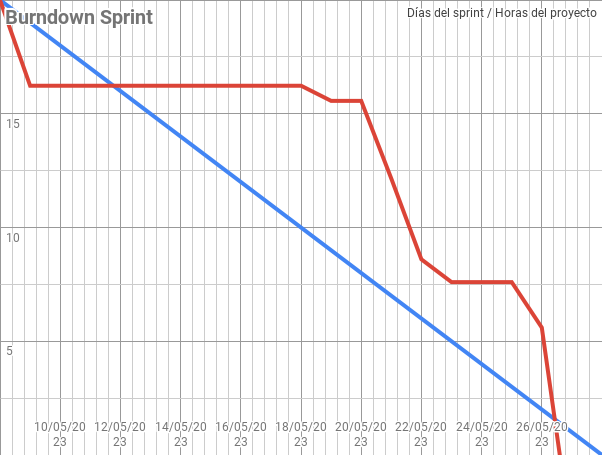
\includegraphics[width=0.46\textwidth]{sprints/Burndown Sprint 8.png}}\qquad
\subfloat[Burndown chart del sprint 9 (periodo del 29/05/2023 al 18/06/2023).]{\label{fig:sprint9}
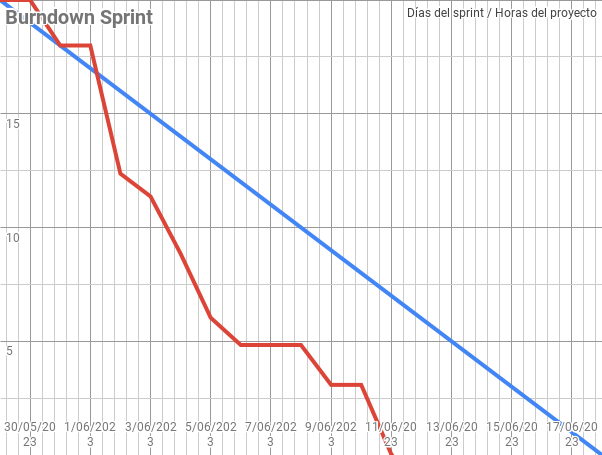
\includegraphics[width=0.46\textwidth]{sprints/Burndown Sprint 9.png}}\qquad
\subfloat[Burndown chart del sprint 10 (periodo del 19/06/2023 al 09/07/2023).]{\label{fig:sprint10}
\includegraphics[width=0.46\textwidth]{sprints/Burndown Sprint 10.png}}\qquad
\subfloat[Burndown chart del sprint 11 (periodo del 10/07/2023 al 30/07/2023).]{\label{fig:sprint11}
\includegraphics[width=0.46\textwidth]{sprints/Burndown Sprint 11.png}}\qquad
\subfloat[Burndown chart del sprint 12 (periodo del 31/07/2023 al 10/08/2023).]{\label{fig:sprint12}
\includegraphics[width=0.46\textwidth]{sprints/Burndown Sprint 12.png}}
\caption{Burdown charts de los seis últimos sprints del proyecto.}
\label{fig:sprints7-12}
\end{figure}

\subsection{Sprint 7 (Figura \ref{fig:sprint7})}

En este caso, la Figura \ref{fig:sprint7} revela que hubo un ritmo de trabajo insuficiente tanto al principio como al final del sprint. Sin embargo, durante todo el tramo central del mismo se estuvo trabajando de manera intensa aunque insuficiente para abarcar toda la cantidad de trabajo asignada a este sprint.

\subsection{Sprint 8 (Figura \ref{fig:sprint8})}

En este octavo sprint podemos apreciar que se realiza más trabajo del planificado en los extremos del periodo considerado gracias a la realización de grandes esfuerzos en días concretos. Esto, en cierto modo, ha servido para compensar parte del trabajo no realizado durante la parte central del sprint.

\subsection{Sprint 9 (Figura \ref{fig:sprint9})}

Podemos ver claramente en la Figura \ref{fig:sprint9} que durante el periodo de tiempo asignado a este sprint se ha realizado mucho más trabajo del planificado. No obstante, realizando un análisis global del proyecto, este exceso de trabajo puede verse como una compensación del trabajo no completado en sprints anteriores.

\subsection{Sprint 10 (Figura \ref{fig:sprint10})}

Durante el décimo sprint se mantuvo una tendencia algo sosegada durante el primer cuarto del mismo. Sin embargo, después se aceleró el ritmo de tal forma que se cortaron la curva de trabajo real y la curva ideal hacia la mitad del sprint. Por último, tras relajarse el ritmo de trabajo se produce una recuperación del mismo, llegando a ser casi ideal hacia el final del sprint.

\subsection{Sprint 11 (Figura \ref{fig:sprint11})}

Al igual que en el noveno sprint, podemos observar que se realiza bastante más trabajo del asignado. Efectivamente, comparando las Figuras \ref{fig:sprint9} y \ref{fig:sprint11} podemos ver que la tendencia es parecida. Esto se debe a que, en las últimas fases del proyecto, se han dedicado una mayor cantidad de horas de trabajo con la finalidad de completarlo.

\subsection{Sprint 12 (Figura \ref{fig:sprint12})}

Este sprint tiene una duración menor a las tres semanas habituales de los sprints anteriores. Su longitud menor se debe a que se trata del último sprint del proyecto o sprint de finalización. Del mismo modo que ocurría en el sprint anterior, la cantidad de horas invertidas en el proyecto supera a la cantidad de horas que se planificaron inicialmente. No obstante, si se analiza desde un punto de vista global, el exceso de horas invertidas en los últimos sprints del proyecto compensa la cantidad de trabajo que no se llegó a completar en sprints anteriores.

\section{Análisis global del proyecto}

Observando el burndown chart global del proyecto (Figura \ref{fig:global}) se puede apreciar que hay algunos tramos de la curva completamente planos correspondientes a periodos de inactividad tal y como se ha mencionado anteriormente. Como consecuencia, puede apreciarse que hasta prácticamente el final del mismo se ha ido por detrás del trabajo planificado. No obstante, al final de su desarrollo se ha realizado más trabajo del estimado, aproximándose cada vez la curva de trabajo real a la curva ideal compensando finalmente la diferencia entre ambas.

Así pues, se puede concluir que globalmente se ha realizado la cantidad de trabajo estimada antes de la finalización del proyecto. Adicionalmente, pese al distanciamiento de la situación ideal en algunos puntos del mismo, se ha logrado mantener bajo control el proyecto durante los diferentes sprints. Finalmente, gracias al seguimiento realizado se han podido valorar en cada punto de su desarrollo los riesgos existentes, tomándose así medidas en relación a éstos, por ejemplo, compensando con trabajo extra las horas no empleadas en periodos anteriores.

\begin{figure}[H]
    \centering
    \includegraphics[width=0.60\textwidth]{sprints/Burndown Proyecto.png}
    \caption{Burndown chart del proyecto (periodo del 12/12/2022 al 10/08/2023).}
    \label{fig:global}
\end{figure}

\ctparttext{
  \color{black}
  \begin{center}
    Análisis de los resultados obtenidos.
  \end{center}
}
\part{Resultados obtenidos}\label{sec:parteV}

\chapter{Análisis de las correlaciones entre las distintas métricas}
\addcontentsline{toc}{chapter}{Análisis de las correlaciones entre las distintas métricas}

En primer, las correlaciones que más nos interesan son las de las distintas métricas con la variable \emph{Grade}. En la Figura \ref{fig:correlations} podemos ver que no todas las métricas correlan con la misma.

\begin{figure}[H]
    \centering
    \includegraphics[width=\textwidth]{correlations.png}
    \caption{Correlaciones existentes entre las distintas métricas y la variable \emph{Grade}.}
    \label{fig:correlations}
\end{figure}

Así pues, vemos que las variables \emph{np} ($p = 0.0127 < 0.05$), \emph{fr} ($p = 0.0378 < 0.05$),    \emph{ps} ($p = 0.0031 < 0.05$) y \emph{sq} ($p = 0.0226 < 0.05$) correlan con la calificación obtenida y que la variable \emph{ns} podría correlar con la variable \emph{Grade} aunque con un grado de certeza menor que el resto ($p = 0.0712 < 0.1$).
\chapter{Perfiles de estudiantes según su rendimiento}\label{sec:chapterXII}
\addcontentsline{toc}{chapter}{Perfiles de estudiantes según su rendimiento}

Debido a la dificultad de predecir de manera exacta la calificación obtenida por los alumnos a partir de las medidas de rendimiento descritas anteriormente, se agruparán las notas en clusters significativos y trataremos de predecir en qué cluster se encuentra la nota de un determinado grupo de alumnos.

\section{Por clusters fijos de notas}

En primer lugar, escogeremos como separación los cuartiles de las calificaciones. Así pues, podemos ver la distribución de los cuartiles en la Figura \ref{fig:boxplotquartilegrade}, donde los límites inferiores de cada una de las cajas son $6.99$, $8.23$, $8.95$ y $9.60$ respectivamente. También puede verse en la Figura \ref{fig:countquartilegrade} el número de grupos que hay en cada cuartil.


\begin{figure}[H]
\centering
\subfloat[Boxplot de las calificaciones por cuartil.]{\label{fig:boxplotquartilegrade}\includegraphics[width=0.47\textwidth]{clustering/boxplotgrade.png}}\qquad
\subfloat[Número de grupos por cuartil.]{\label{fig:countquartilegrade}\includegraphics[width=0.47\textwidth]{clustering/countquartilegrade.png}}%
\caption{Resultados obtenidos tras agrupar las caficaciones por cuartiles.}
\label{fig:quartilegradeclustering}
\end{figure}

Sin embargo, en la Figura \ref{fig:boxplotquartilegrade} y en la Figura \ref{fig:frequenciesgrade}, donde se representan cómo de frecuentes son cada una de las calificaciones obtenidas, notamos la presencia de un outlier.

\begin{figure}[H]
    \centering
    \includegraphics[width=0.6\textwidth]{clustering/frequencygrade.png}
    \caption{Calificaciones obtenidas por los distintos grupos. El límite de los cuartiles se ha indicado con líneas verticales negras.}
    \label{fig:frequenciesgrade}
\end{figure}

En la Figura \ref{fig:densitybyfactorquartilegrade} vemos las funciones de densidad por cuartil. Prestaremos especial atención a los grupos del cluster \texttt{Q1} (el de las peores calificaciones al que le añadimos el outlier) puesto que son los que peor rendimiento han mostrado.

\begin{figure}[H]
    \centering
    \includegraphics[width=0.6\textwidth]{clustering/densitybyfactorquartilegrade.png}
    \caption{Funciones de densidad de las calificaciones obtenidas por cluster.}
    \label{fig:densitybyfactorquartilegrade}
\end{figure}

\section{Por clusters dinámicos de notas}

Se agruparán los datos usando el algoritmo de las K-medias sobre la variable \emph{Grade}. Para decidir el número de clusters en el que agruparemos los datos, se usarán métodos gráficos. Como podemos ver en las Figuras \ref{fig:indiceshubert} y \ref{fig:indicesdindex}, el número óptimo de particiones podría ser $3$ o $5$. Para decidir entre un número de clusters u otro se realizarán los dos agrupamientos y nos quedaremos con el de menor error.

\begin{figure}[H]
    \centering
    \includegraphics[width=\textwidth]{clustering/Hubert.png}
    \caption{Valores estadísticos de Hubert.}
    \label{fig:indiceshubert}
\end{figure}

\begin{figure}[H]
    \centering
    \includegraphics[width=\textwidth]{clustering/Dindex.png}
    \caption{Valores de Dindex.}
    \label{fig:indicesdindex}
\end{figure}

Aplicando el algoritmo de las K-medias para $K = 2$ (Figura \ref{fig:KMeans2}) y para $K = 3$ (Figura \ref{fig:KMeans3}), vemos que hay una gran diferencia entre la precisión de uno y otro (para $K = 2$ se tiene $\texttt{accuracy} = 0.6978412$ mientras que para $K = 3$ se tendrá $\texttt{accuracy} = 0.8585982$). Además, como puede apreciarse en las Figuras \ref{fig:KMeans2} y \ref{fig:KMeans3}, seguimos teniendo un outlier en ambos casos.

\begin{figure}[H]
    \centering
    \includegraphics[width=0.6\textwidth]{clustering/KMeans2.png}
    \caption{Particiones obtenidas con $K = 2$.}
    \label{fig:KMeans2}
\end{figure}

\begin{figure}[H]
    \centering
    \includegraphics[width=0.6\textwidth]{clustering/KMeans3.png}
    \caption{Particiones obtenidas con $K = 3$.}
    \label{fig:KMeans3}
\end{figure}

La distribución de la variable \emph{Grade} dentro de cada partición puede verse en las Figuras \ref{fig:KMeans2boxplot} y \ref{fig:KMeans3boxplot} mientras que el número de grupos que hay en las particiones puede verse en las Figuras \ref{fig:KMeans2count} y \ref{fig:KMeans3count}.

\begin{figure}[H]
\centering
\subfloat[Boxplot de cada una de las particiones.]{\label{fig:KMeans2boxplot}\includegraphics[width=0.47\textwidth]{clustering/KMeans2boxplot.png}}\qquad
\subfloat[Número de grupos por partición.]{\label{fig:KMeans2count}\includegraphics[width=0.47\textwidth]{clustering/KMeans2count.png}}%
\caption{Resultados obtenidos tras aplicar el algoritmo de las $K$-Medias con $K = 2$.}
\label{fig:KMeans2details}
\end{figure}

\begin{figure}[H]
\centering
\subfloat[Boxplot de cada una de las particiones.]{\label{fig:KMeans3boxplot}\includegraphics[width=0.47\textwidth]{clustering/KMeans3boxplot.png}}\qquad
\subfloat[Número de grupos por partición.]{\label{fig:KMeans3count}\includegraphics[width=0.47\textwidth]{clustering/KMeans3count.png}}%
\caption{Resultados obtenidos tras aplicar el algoritmo de las $K$-Medias con $K = 3$.}
\label{fig:KMeans3details}
\end{figure}

Por último, para cinco particiones (Figura \ref{fig:KMeans5}) se tendrá $\texttt{accuracy} = 0.9474439$. Es decir, tenemos más precisión con cinco particiones y ya no tenemos outliers. Nos centramos en estudiar los grupos de los dos primeros clusters (aquellos grupos con una nota inferior a $7.34$).

\begin{figure}[H]
    \centering
    \includegraphics[width=0.6\textwidth]{clustering/KMeans5.png}
    \caption{Particiones obtenidas con $K = 5$.}
    \label{fig:KMeans5}
\end{figure}

\begin{figure}[H]
\centering
\subfloat[Boxplot de cada una de las particiones.]{\label{fig:KMeans5boxplot}\includegraphics[width=0.47\textwidth]{clustering/KMeans5boxplot.png}}\qquad
\subfloat[Número de grupos por partición.]{\label{fig:KMeans5count}\includegraphics[width=0.47\textwidth]{clustering/KMeans5count.png}}%
\caption{Resultados obtenidos tras aplicar el algoritmo de las $K$-Medias con $K = 5$.}
\label{fig:KMeans5details}
\end{figure}

\section{Por clusters aproximados de rendimiento}

De las medidas de rendimiento estudiadas en el Capítulo \ref{chapter:rendimiento}, nos quedaremos con aquellas que correlan con la variable \emph{Grade} (\emph{np}, \emph{fr}, \emph{ps}, \emph{sq} y \emph{ns}). Así pues, se definirá una nueva métrica, a la que denotaremos por \emph{fm}, como la suma de las medidas de rendimiento \emph{p}, \emph{fr}, \emph{ps}, \emph{sq} y \emph{s}. En la Figura \ref{fig:correlationfm} vemos que \emph{fm} no correla con la variable \emph{Grade}.

\begin{figure}[H]
    \centering
    \includegraphics[width=0.8\textwidth]{clustering/fm.png}
    \caption{Regresión lineal para aproximar la relación de dependencia entre la variable \emph{fm} y la variable \emph{Grade}.}
    \label{fig:correlationfm}
\end{figure}

A continuación, se agruparán los datos usando el algoritmo de las K-medias sobre la variable \emph{fm}. Para decidir el número de clusters en el que agruparemos los datos, se usarán métodos gráficos. Como podemos ver en las Figuras \ref{fig:indiceshubertfm} y \ref{fig:indicesdindexfm}, el número óptimo de particiones podría ser $4$ o $7$. Para decidir entre un número de clusters u otro se realizarán los dos agrupamientos y nos quedaremos con el de menor error.

\begin{figure}[H]
    \centering
    \includegraphics[width=\textwidth]{clustering/Hubertfm.png}
    \caption{Valores estadísticos de Hubert.}
    \label{fig:indiceshubertfm}
\end{figure}

\begin{figure}[H]
    \centering
    \includegraphics[width=\textwidth]{clustering/Dindexfm.png}
    \caption{Valores de Dindex.}
    \label{fig:indicesdindexfm}
\end{figure}

Aplicando el algoritmo de las K-medias para $K = 4$ (Figura \ref{fig:KMeans4}) y para $K = 7$ (Figura \ref{fig:KMeans7}), vemos que hay una gran diferencia la precisión de uno y otro (para $K = 4$ se tiene $\texttt{accuracy} = 0.921137$ mientras que para $K = 7$ se tendrá $\texttt{accuracy} = 0.9772655$). Además, en la Figura \ref{fig:KMeans4} podemos notar la presencia de outliers mientras que en la Figura \ref{fig:KMeans7} no.

\begin{figure}[H]
    \centering
    \includegraphics[width=0.6\textwidth]{clustering/outliersfm.png}
    \caption{Particiones obtenidas con $K = 4$. Como podemos ver, se observa la presencia de outliers ($260.804$, $63.173$, $106.379$ y $261.823$).}
    \label{fig:KMeans4}
\end{figure}

\begin{figure}[H]
    \centering
    \includegraphics[width=0.6\textwidth]{clustering/KMeans7fm.png}
    \caption{Particiones obtenidas con $K = 7$. No hay ningún outlier.}
    \label{fig:KMeans7}
\end{figure}

La distribución de la variable \emph{Grade} dentro de cada partición puede verse en las Figuras \ref{fig:KMeans4boxplot} y \ref{fig:KMeans7boxplot} mientras que el número de grupos que hay en las particiones puede verse en las Figuras \ref{fig:KMeans4count} y \ref{fig:KMeans7count}.

\begin{figure}[H]
\centering
\subfloat[Boxplot de cada una de las particiones.]{\label{fig:KMeans4boxplot}\includegraphics[width=0.47\textwidth]{clustering/KMeansfmboxplot.png}}\qquad
\subfloat[Número de grupos por partición.]{\label{fig:KMeans4count}\includegraphics[width=0.47\textwidth]{clustering/KMeansfmcount.png}}%
\caption{Resultados obtenidos tras aplicar el algoritmo de las $K$-Medias con $K = 4$.}
\label{fig:KMeans4details}
\end{figure}

\begin{figure}[H]
\centering
\subfloat[Boxplot de cada una de las particiones.]{\label{fig:KMeans7boxplot}\includegraphics[width=0.47\textwidth]{clustering/KMeans7boxplot.png}}\qquad
\subfloat[Número de grupos por partición.]{\label{fig:KMeans7count}\includegraphics[width=0.47\textwidth]{clustering/KMeans7count.png}}%
\caption{Resultados obtenidos tras aplicar el algoritmo de las $K$-Medias con $K = 7$.}
\label{fig:KMeans7details}
\end{figure}

\section{Clustering mediante las propiedades espectrales de los grafos}
\subsection{Clustering mediante el coeficiente LOGLAP09}

Ahora, se ha decidido se asociar los datos usando el algoritmo de las K-medias sobre la variable \emph{LOGLAP09}. Para decidir el número de clusters en el que agruparemos los datos, se usarán métodos gráficos. Como podemos ver en las Figuras \ref{fig:indiceshubertLAP} y \ref{fig:indicesdindexLAP}, se ha decidido agrupar los datos en $5$ clusters (Figura \ref{fig:KMeansLAP}, $\texttt{accuracy} = 0.9673813$).

\begin{figure}[H]
    \centering
    \includegraphics[width=\textwidth]{clustering/HubertLAP.png}
    \caption{Valores estadísticos de Hubert.}
    \label{fig:indiceshubertLAP}
\end{figure}

\begin{figure}[H]
    \centering
    \includegraphics[width=\textwidth]{clustering/DindexLAP.png}
    \caption{Valores de Dindex.}
    \label{fig:indicesdindexLAP}
\end{figure}

\begin{figure}[H]
    \centering
    \includegraphics[width=0.6\textwidth]{clustering/partitionsLOGLAP09.png}
    \caption{Particiones obtenidas con $K = 5$. No hay ningún outlier.}
    \label{fig:KMeansLAP}
\end{figure}

La distribución de la variable \emph{Grade} dentro de cada partición puede verse en la Figura \ref{fig:KMeansLAPboxplot} mientras que el número de grupos que hay en las particiones puede verse en la Figura \ref{fig:KMeansLAPcount}.

\begin{figure}[H]
\centering
\subfloat[Boxplot de cada una de las particiones.]{\label{fig:KMeansLAPboxplot}\includegraphics[width=0.47\textwidth]{clustering/KMeansLAPboxplot.png}}\qquad
\subfloat[Número de grupos por partición.]{\label{fig:KMeansLAPcount}\includegraphics[width=0.47\textwidth]{clustering/KMeansLAPcount.png}}%
\caption{Resultados obtenidos tras aplicar el algoritmo de las $K$-Medias con $K = 5$.}
\label{fig:KMeansLAPdetails}
\end{figure}

\subsection{Clustering mediante el coeficiente DAG}

\subsection{¿Quiénes son los grupos en riesgo?}\label{sec:badstudents}

El objetivo principal de este enfoque es tratar de identificar a los estudiantes que tienen dificultades en resolver las tareas propuestas en el laboratorio virtual porque ellos, y no los alumnos ordinarios, requieren la mayor parte de la atención de del profesor para poder alcanzar un $100\%$ de éxito. Pero, ¿quiénes son?

En principio nos vamos a centrar en los alumnos con el cuartil más bajo de la nota, es decir, aquellos cuya nota está por debajo, como mínimo, del $75\%$ de las demás calificaciones (Figura \ref{fig:frequenciesgrade}). Sin embargo, dada la dinámica de las calificaciones cada año (Figura \ref{fig:boxplotachieveryear}), podemos ver que este primer cuartil podría no ser muy preciso. En su lugar, se ha usado la función \texttt{KMeans} en R para dividir el rango de calificaciones en $5$ intervalos con una precisión del $95\%$ en las interdependencias e intradependencias de los $5$ clusters. En la partición obtenida mediante KMeans, hay dos grupos cuyas calificaciones son son estrictamente inferiores a $8$ (Figura \ref{fig:KMeans5}). Vamos a centrarnos en estos a grupos, que se denominarán \emph{``LOW''}. Por el contrario, el resto de grupos se llamarán \emph{``GOOD''}.

Este conjunto de datos podría procesarse como un único cluster de datos y sólo tendríamos una visión del final del periodo de las prácticas, que podría ser informativo, pero no útil para una intervención temprana. Con el fin de preparar el conjunto de datos para que sea útil cuanto antes y no sólo al final de la práctica, se va a estratificar por niveles donde cada nivel $i \in [3,9]$ está marcado por la primera vez que el problema (o asignación) $i$ se ha resuelto (Figura \ref{fig:stratification}). Por lo tanto, alcanzar nivel $9$ significa que se han completado todas las tareas.

\begin{figure}[H]
    \centering
    \includegraphics[width=\textwidth]{clustering/stratification.png}
    \caption{Estratificación del conjunto de datos en $10$ episodios consecutivos. Uno para la consecución de cada uno de los $9$ problemas, más un último episodio hasta el final de la práctica.}
    \label{fig:stratification}
\end{figure}

Así pues, tenemos un conjunto de datos muy fiable, reforzado con evidencias de que no hay sesgos a lo largo de los años. También tenemos una partición preliminar sólida y significativa de las calificaciones y un nuevo conjunto de funciones en forma de campana de uso general para identificar estas particiones (Sección \ref{sec:complexity}). ¿Qué podría salir mal?
\chapter{Clasificación de los grupos de alumnos según su rendimiento}\label{sec:chapterXIII}
\addcontentsline{toc}{chapter}{Clasificación de los grupos de alumnos según su rendimiento}

Para realizar la identificación de los subconjuntos de alumnos definidos en la Sección \ref{sec:badstudents}, se empleará el algoritmo de clasificación de Quinlan C5.0 \cite{Quinlan:See5C5}, que no es más que una herramienta de aprendizaje supervisado que genera un árbol de decisión o un conjunto de reglas. Así pues, las distintas categorías en las que se clasificarán a los grupos vendrán dadas en las hojas de dichos árboles y en los consecuentes de las reglas respectivamente. El clasificador estadístico C5.0 se basa en el concepto de entropía, seleccionando primero aquellas características cuyos valores se diferencian más entre distintas categorías de grupos de alumnos.

Se utilizarán como variables de entrada del clasificador tanto las medidas clásicas de rendimiento presentadas en el Capítulo \ref{chapter:rendimiento} como las medidas grafo-teóricas (Sección \ref{sec:complexity}). Por su parte, como categorías de salida, tendremos tanto una única partición en alumnos ``LOW'', que se supone que requieren más esfuerzo para superar el laboratorio, como las cinco particiones que se muestran en la Figura \ref{fig:KMeans5}.

Dado que hay muy pocos registros ($77$ en cada nivel), el problema de clasificación va a ser difícil y, con el fin de aumentar las evidencias requeridas por C5.0 para trabajar, el conjunto de datos se agrupará cada tres niveles consecutivos. Así pues, por un lado, agruparemos los niveles $3$, $4$ y $5$ para realizar predicciones al principio de la práctica y, por otro lado, agruparemos los niveles $8$, $9$ y $10$. Así pues, las siguientes secciones se dividrán en dos subapartados, dependiendo de la parte del dataset que estemos utilizando para entrenar el clasificador.

\section{Clasificación empleando las métricas clásicas de rendimiento}



\section{Clasificación empleando las medidas de complejidad de propósito general}

\subsection{Clasificación empleando los niveles 3, 4 y 5}

El resultado es que C5.0 obtiene un conjunto de reglas capaz de clasificar exactamente los $35$ de los $36$ casos de grupos \emph{``LOW''} del nivel $3$ en adelante, es decir, a partir de un tercio del periodo de tiempo dedicado a la práctica, con un $p$ value $p = 3.843e-16$ estadísticamente muy relevante (Figura \ref{fig:cm2}). Además, las reglas obtenidas (Figura \ref{rules2}) tienen pleno sentido. Por ejemplo, la regla $7$ dice: ``Un grupo está en riesgo si está centrado en los problemas con numeración alta (\texttt{Be > 6})''. O la regla $3$ que dice ``Un grupo está en riesgo si no se ha centrado por igual en todos los problemas (\texttt{Ba > 3.366005}) y recorre caminos menos largos en media (\texttt{WDag > -4.317488}) teniendo en cuenta que el valor de máxima probabilidad de la métrica $WDag$ es $-4.19$.

\begin{figure}[H]
\centering
\begin{tikzpicture}
  \node (matrix)  {$\begin{array}{c|cc}
			 & GOOD & LOW \\ \hline
        GOOD & 186  & 1 \\
        LOW & 0 & 35
\end{array}$};
  \node[above of= matrix, node distance=0.5cm, yshift=1cm,font=\color{black}] {\textbf{Referencia}};
  \node[left of= matrix, node distance=3.5cm, rotate=90, anchor=center,yshift=-0.7cm,font=\color{black}] {\textbf{Predicción}};
  % Tabular environment for additional text
  \node[below of=matrix, node distance=2.5cm,font=\color{gray}]{
    \begin{tabular}{l}
      \texttt{Accuracy : 0.9955} \\
      \texttt{95\% CI : (0.9752, 0.9999)} \\
      \texttt{No Inform. Rate : 0.8378} \\
      \texttt{P-Value : 3.843e-16 }
    \end{tabular}
  };
\end{tikzpicture}
\caption{Aprendiendo a identificar a los grupos \emph{``LOW''}, es decir, aquellos con una puntuación inferior a $8.1$ sobre $10$.}
\label{fig:cm2}
\end{figure}

\begin{tcolorbox}[title=Reglas de clasificación para identificar grupos de tipo \emph{``LOW''}.]
  %add special color box to list of listings
  \makeatletter
  \addcontentsline{lol}{subsection}{\kvtcb@title}
  \makeatother
\begin{multicols}{2}
    \begin{minted}{R}
Rule 11/1: (17.8, lift 1.5)
	Ba > 9.26712
	->  class GOOD  [0.949]

Rule 11/2: (200.7/68.3, lift 1.0)
	De > 0.0952381
	->  class GOOD  [0.658]

Rule 11/3: (8.5/0.3, lift 2.5)
	WDag > -4.317488
	Ba > 3.366005
	->  class LOW  [0.880]

Rule 11/4: (5, lift 2.4)
	Dm <= 1.2
	Ef <= 4
	St > 1.791759
	->  class LOW  [0.858]

Rule 11/5: (8.3/0.6, lift 2.4)
	De <= 0.0989011
	Ef <= 4
	Ba <= 9.26712
	->  class LOW  [0.850]

Rule 11/6: (9.4/1.1, lift 2.3)
	De > 0.1153846
	Ef > 3
	Ef <= 4
	WDag <= -6.612041
	Ba > 3.366005
	->  class LOW  [0.818]

Rule 11/7: (3.4, lift 2.3)
	Be > 6
	->  class LOW  [0.814]

Rule 11/8: (13.3/2.3, lift 2.2)
	De <= 0.0952381
	Ba <= 9.26712
	->  class LOW  [0.783]

Rule 11/9: (19.9/5.4, lift 2.0)
	Dm <= 1.222222
	Ef <= 3
	St > 0.6931472
	Ba <= 9.26712
	->  class LOW  [0.707]
    \end{minted}
  \end{multicols}
\label{rules2}
\end{tcolorbox}

Pero no sólo esto, ¿podríamos dar un gran paso y predecir no sólo equipos \emph{``LOW''}/\emph{``GOOD''}, sino también un límite inferior y superior de sus calificaciones finales, y adivinar en cuál de los $5$ intervalos de la Figura \ref{fig:KMeans5} se encuentran? La respuesta es, felizmente, sí.

Efectivamente, C5.0 obtiene un conjunto de reglas (Figura \ref{rules5}) capaz de clasificar exactamente todos los grupos dentro de su correspondiente intervalo de calificaciones del nivel $3$ en adelante, es decir, a partir de un tercio del periodo de tiempo dedicado a la práctica, con un $p$ value $p < 2.2e-16$ estadísticamente muy relevante (Figura \ref{fig:cm5}).

\begin{figure}[H]
\centering
\begin{tikzpicture}
  \node (matrix)  {$\begin{array}{c|ccccc}
                         & \left[6.46,6.99\right] & \left[7.39,7.96\right] & \left[8.1,8.64\right] & \left[8.79,9.35\right] & \left[9.44,10\right]\\ \hline
        \left[6.46,6.99\right] & 6 & 0 & 0 & 0 & 0 \\
        \left[7.39,7.96\right] & 0 & 30 & 0 & 0 & 0 \\
        \left[8.1,8.64\right] & 0 & 0 & 42 & 0 & 0 \\
        \left[8.79,9.35\right] & 0 & 0 & 0 & 69 & 0 \\
        \left[9.44,10\right] & 0 & 0 & 0 & 0 & 75
\end{array}$};
  \node[above of= matrix, node distance=1.5cm, yshift=1cm,font=\color{black}] {\textbf{Referencia}};
  \node[left of= matrix, node distance=8cm, rotate=90, anchor=center,yshift=-0.7cm,font=\color{black}] {\textbf{Predicción}};
  % Tabular environment for additional text
  \node[below of=matrix, node distance=3.5cm,font=\color{gray}]{
    \begin{tabular}{l}
      \texttt{Accuracy : 1} \\
      \texttt{95\% CI : (0.9835, 1)} \\
      \texttt{No Inform. Rate : 0.3378} \\
      \texttt{P-Value : < 2.2e-16 }
    \end{tabular}
  };
\end{tikzpicture}
\caption{Aprendiendo a identificar a los grupos de prácticas con un intervalo de notas (Figura \ref{fig:KMeans5}).}
\label{fig:cm5}
\end{figure}

\begin{tcolorbox}[title=Reglas de clasificación para identificar intervalos de notas.]
  %add special color box to list of listings
  \makeatletter
  \addcontentsline{lol}{subsection}{\kvtcb@title}
  \makeatother
\begin{multicols}{3}
    \begin{minted}[fontsize=\scriptsize]{R}
Rule 99/1: (4.6, lift 4.7)
        We <= 0.01080108
        Ba > 3.366005
        ->  class [7.39,7.96]  [0.848]
Rule 99/2: (3.4, lift 4.5)
        We <= 0.2018018
        WDag <= -6.478509
        Be <= 1
        ->  class [7.39,7.96]  [0.815]
Rule 99/3: (9.4/2.2, lift 4.0)
        We <= 0.2702703
        St > 1.791759
        St <= 2.079442
        ->  class [7.39,7.96]  [0.721]
Rule 99/4: (11.1/3.5, lift 3.6)
        Cl > 0.2619048
        Di <= -4.219508
        We > 0.2131148
        We <= 0.2702703
        St > 0
        WDag <= -5.901418
      ->  class [7.39,7.96] [0.653]
Rule 99/5: (6.5/2.1, lift 3.5)
        De <= 0.0952381
        We <= 0.1321739
        ->  class [7.39,7.96]  [0.630]
Rule 99/6: (10.2/6.1, lift 2.3)
        St > 5.257495
        ->  class [7.39,7.96]  [0.414]
Rule 99/7: (7.6/0.5, lift 3.6)
        We > 0.2702703
        St <= 0
        WDag > -7.122867
      ->  class [8.1,8.64] [0.840]
Rule 99/8: (4.1, lift 3.6)
        We <= 0.2702703
        St > 2.079442
        WDag <= -5.296464
        Be <= 2
        ->  class [8.1,8.64]  [0.837]
Rule 99/9: (9.4/1.8, lift 3.2)
        Cl > 0.4095238
        We <= 0.2702703
        St > 0
        St <= 1.791759
        Dag > -5.204007
        Ba > 5.925958
        ->  class [8.1,8.64]  [0.751]
Rule 99/10: (6.3/1.9, lift 2.8)
        De <= 0.0952381
        We > 0.1321739
        ->  class [8.1,8.64]  [0.658]
Rule 99/11: (17.1/6, lift 2.7)
        De > 0.0952381
        We > 0.01080108
        We <= 0.04410441
        Ba > 3.366005
        ->  class [8.1,8.64]  [0.633]
Rule 99/12: (6.7/2.3, lift 2.7)
        We <= 0.01080108
        Ba <= 3.366005
        ->  class [8.1,8.64]  [0.621]   
Rule 99/13: (187.3/131.4, lift 1.1)
        We > 0.04410441
        ->  class [8.79,9.35]  [0.301]       
Rule 99/14: (9.2, lift 3.1)
        Cl > 0.2619048
        Di <= -4.219508
        We > 0.1415628
        We <= 0.2131148
        St > 0
        St <= 2.079442
        Ba <= 5.925958
        ->  class [9.44,10]  [0.911]
Rule 99/15: (7.1, lift 3.0)
        We > 0.2018018
        We <= 0.2287122
        St <= 0
        ->  class [9.44,10]  [0.890]
Rule 99/16: (6.8, lift 3.0)
        We > 0.2702703
        St <= 0
        WDag > -8.251143
        WDag <= -7.122867
        ->  class [9.44,10]  [0.886]
Rule 99/17: (5.5, lift 2.9)
        We > 0.2131148
        St <= 2.079442
        WDag > -5.901418
        ->  class [9.44,10]  [0.867]
Rule 99/18: (5.1, lift 2.9)
        We > 0.01080108
        We <= 0.04410441
        Ba <= 3.366005
        ->  class [9.44,10]  [0.860]
Rule 99/19: (4.7, lift 2.9)
        We > 0.04410441
        St <= 0
        WDag > -5.755742
        ->  class [9.44,10]  [0.851]
Rule 99/20: (11.5/1.3, lift 2.8)
        Dm <= 1
        Di <= -4.219508
        We > 0.04410441
        We <= 0.2131148
        St > 0
        Ba <= 5.925958
        ->  class [9.44,10]  [0.832]
Rule 99/21: (9.1/1.7, lift 2.6)
        Cl > 0.2792208
        We > 0.2702703
        St > 1.386294
        Dag > -5.204007
        Be > 1
        ->  class [9.44,10]  [0.759]
Rule 99/22: (10.6/2.6, lift 2.4)
        Cl <= 0.4095238
        De > 0.0952381
        St <= 1.791759
        Be > 2
        Ba > 5.925958
        ->  class [9.44,10]  [0.718]
    \end{minted}
  \end{multicols}
\label{rules5}
\end{tcolorbox}

\subsection{Clasificación empleando los niveles 8, 9 y 10}

El resultado es que C5.0 obtiene un conjunto de reglas capaz de clasificar exactamente los $36$ casos de grupos \emph{``LOW''} del nivel $8$ en adelante, es decir, a partir del último tercio del periodo de tiempo dedicado a la práctica, con un $p$ value $p < 2.2e-16$ estadísticamente muy relevante (Figura \ref{fig:cm3}). Además, las reglas obtenidas (Figura \ref{rules3}) tienen pleno sentido como en el caso anteriormente visto.

\begin{figure}[H]
\centering
\begin{tikzpicture}
  \node (matrix)  {$\begin{array}{c|cc}
			 & GOOD & LOW \\ \hline
        GOOD & 186  & 0 \\
        LOW & 0 & 36
\end{array}$};
  \node[above of= matrix, node distance=0.5cm, yshift=1cm,font=\color{black}] {\textbf{Referencia}};
  \node[left of= matrix, node distance=3.5cm, rotate=90, anchor=center,yshift=-0.7cm,font=\color{black}] {\textbf{Predicción}};
  % Tabular environment for additional text
  \node[below of=matrix, node distance=2.5cm,font=\color{gray}]{
    \begin{tabular}{l}
      \texttt{Accuracy : 1} \\
      \texttt{95\% CI : (0.9835, 1)} \\
      \texttt{No Inform. Rate : 0.8378} \\
      \texttt{P-Value : < 2.2e-16}
    \end{tabular}
  };
\end{tikzpicture}
\caption{Aprendiendo a identificar a los grupos \emph{``LOW''}, es decir, aquellos con una puntuación inferior a $8.1$ sobre $10$.}
\label{fig:cm3}
\end{figure}

\begin{tcolorbox}[title=Reglas de clasificación para identificar grupos de tipo \emph{``LOW''}.]
  %add special color box to list of listings
  \makeatletter
  \addcontentsline{lol}{subsection}{\kvtcb@title}
  \makeatother
\begin{multicols}{2}
    \begin{minted}{R}
Rule 99/1: (8.3, lift 1.3)
	St <= 1.791759
	->  class GOOD  [0.903]

Rule 99/2: (8.3, lift 1.3)
	Be <= 1
	Ba <= 7.664816
	->  class GOOD  [0.903]

Rule 99/3: (81.3/11, lift 1.3)
	We > 0.4208696
	->  class GOOD  [0.855]

Rule 99/4: (72.7/13, lift 1.2)
	Cl <= 0.2771242
	We > 0.06390639
	We <= 0.4208696
	Be > 4
	->  class GOOD  [0.812]

Rule 99/5: (28.1/1.9, lift 2.8)
	We <= 0.4208696
	St > 1.791759
	Be <= 4
	Ba > 7.664816
	->  class LOW  [0.905]

Rule 99/6: (6.9, lift 2.7)
	Di > -8.386857
	St > 15.46906
	->  class LOW  [0.883]

Rule 99/7: (4.8, lift 2.6)
	Cl > 0.2771242
	Be > 4
	->  class LOW  [0.852]

Rule 99/8: (28.7/4.1, lift 2.6)
	We <= 0.4208696
	St > 1.791759
	Be > 1
	Be <= 4
	->  class LOW  [0.834]

Rule 99/9: (5.3/0.4, lift 2.5)
	We <= 0.06390639
	Be > 4
	->  class LOW  [0.815]
    \end{minted}
  \end{multicols}
\label{rules3}
\end{tcolorbox}

Adicionalmente, C5.0 obtiene un conjunto de reglas (Figura \ref{rules6}) capaz de clasificar exactamente todos los grupos dentro de su correspondiente intervalo de calificaciones del nivel $8$ en adelante, es decir, a partir del último tercio del periodo de tiempo dedicado a la práctica, con un $p$ value $p < 2.2e-16$ estadísticamente muy relevante (Figura \ref{fig:cm6}).

\begin{figure}[H]
\centering
\begin{tikzpicture}
  \node (matrix)  {$\begin{array}{c|ccccc}
                         & \left[6.46,6.99\right] & \left[7.39,7.96\right] & \left[8.1,8.64\right] & \left[8.79,9.35\right] & \left[9.44,10\right]\\ \hline
        \left[6.46,6.99\right] & 6 & 0 & 0 & 0 & 0 \\
        \left[7.39,7.96\right] & 0 & 51 & 0 & 0 & 0 \\
        \left[8.1,8.64\right] & 0 & 0 & 54 & 0 & 0 \\
        \left[8.79,9.35\right] & 0 & 0 & 0 & 39 & 0 \\
        \left[9.44,10\right] & 0 & 0 & 0 & 0 & 72
\end{array}$};
  \node[above of= matrix, node distance=1.5cm, yshift=1cm,font=\color{black}] {\textbf{Referencia}};
  \node[left of= matrix, node distance=8cm, rotate=90, anchor=center,yshift=-0.7cm,font=\color{black}] {\textbf{Predicción}};
  % Tabular environment for additional text
  \node[below of=matrix, node distance=3.5cm,font=\color{gray}]{
    \begin{tabular}{l}
      \texttt{Accuracy : 1} \\
      \texttt{95\% CI : (0.9835, 1)} \\
      \texttt{No Inform. Rate : 0.3243} \\
      \texttt{P-Value : < 2.2e-16 }
    \end{tabular}
  };
\end{tikzpicture}
\caption{Aprendiendo a identificar a los grupos de prácticas con un intervalo de notas (Figura \ref{fig:KMeans5}).}
\label{fig:cm6}
\end{figure}

\begin{tcolorbox}[title=Reglas de clasificación para identificar intervalos de notas.]
  %add special color box to list of listings
  \makeatletter
  \addcontentsline{lol}{subsection}{\kvtcb@title}
  \makeatother
\begin{multicols}{3}
    \begin{minted}[fontsize=\scriptsize]{R}
Rule 99/1: (5.8, lift 24.4)
	De > 0.0992647
	We <= 0.2315271
	Dag <= -5.723585
	Ba > 6.816384
	->  class [6.46,6.99]  [0.871]

Rule 99/2: (8, lift 3.9)
	Dm > 2.666667
	Di > -8.386857
	Di <= -8.193677
	->  class [7.39,8.23]  [0.900]

Rule 99/3: (4.1, lift 3.7)
	De <= 0.1520468
	Dm > 2.666667
	->  class [7.39,8.23]  [0.837]

Rule 99/4: (5.7/0.3, lift 3.6)
	Cl > 0.2444444
	We > 0.409966
	Ba > 5.982207
	Ba <= 8.747471
	->  class [7.39,8.23]  [0.831]

Rule 99/5: (8/0.8, lift 3.6)
	Dm > 2.666667
	Di <= -8.193677
	We > 0.409966
	Dag > -5.834811
	WDag <= -2.246848
	->  class [7.39,8.23]  [0.822]

Rule 99/6: (7.9/1.4, lift 3.3)
	Cl > 0.2820513
	We <= 0.409966
	St > 1.098612
	->  class [7.39,8.23]  [0.759]

Rule 99/7: (4.7/0.9, lift 3.2)
	Cl <= 0.1421437
	Be <= 1
  ->  class [7.39,8.23] [0.723]

Rule 99/8: (71.1/45.1, lift 1.6)
	Dag <= -5.723585
	Ba > 6.816384
	->  class [7.39,8.23]  [0.369]

Rule 99/9: (7.9/0.5, lift 3.4)
	De > 0.1520468
	Di <= -8.386857
	We > 0.409966
	Dag <= -5.834811
	WDag <= -2.246848
	->  class [8.4,8.94]  [0.844]

Rule 99/10: (3.7, lift 3.4)
	Dm > 2.666667
	Di > -8.193677
	->  class [8.4,8.94]  [0.824]

Rule 99/11: (2.9, lift 3.3)
	Cl <= 0.2582892
	Di > -7.669682
	WDag > -4.185531
  ->  class [8.4,8.94] [0.796]

Rule 99/12: (8.7/1.2, lift 3.2)
	Cl <= 0.1728291
	We > 0.2315271
	We <= 0.409966
	Dag <= -5.723585
	Ba > 6.816384
	->  class [8.4,8.94]  [0.795]

Rule 99/13: (6/0.8, lift 3.2)
	Cl > 0.2582892
	Cl <= 0.2820513
	We <= 0.409966
	St > 1.098612
	Be <= 5
	->  class [8.4,8.94]  [0.772]

Rule 99/14: (8.4/3, lift 2.5)
	Ba <= 4.54026
	->  class [8.4,8.94]  [0.618]

Rule 99/15: (11.8/4.6, lift 2.4)
	Dm <= 2.666667
	Be <= 3
	Ba <= 5.982207
	->  class [8.4,8.94]  [0.592]

Rule 99/16: (31.7/18, lift 1.8)
	Dm <= 2.666667
	Dag > -5.834811
	Ba > 8.747471
	->  class [8.4,8.94]  [0.437]

Rule 99/17: (3.4, lift 3.5)
	We <= 0.409966
	Dag > -5.834811
	Dag <= -5.723585
	WDag <= -3.212575
	Ba <= 6.816384
  ->  class [8.98,9.44] [0.816]

Rule 99/18: (3.4, lift 3.5)
	Dm <= 2.666667
	We > 0.409966
	Dag <= -5.834811
	Ba > 8.747471
	->  class [8.98,9.44]  [0.815]

Rule 99/19: (27.8/4.5, lift 3.5)
	Cl <= 0.2582892
	Di > -7.669682
	We <= 0.409966
	St > 1.098612
	WDag > -6.650347
	WDag <= -4.185531
  ->  class [8.98,9.44] [0.815]

Rule 99/20: (6.9/1.3, lift 3.2)
	Cl <= 0.1421437
	Dm <= 2.666667
	We > 0.409966
	Be > 1
  ->  class [8.98,9.44] [0.748]

Rule 99/21: (18.7/6.1, lift 2.8)
	We <= 0.409966
	Dag <= -5.834811
	Ba <= 6.816384
  ->  class [8.98,9.44] [0.655]

Rule 99/22: (5.7, lift 3.4)
	Cl > 0.1705797
	Cl <= 0.2291667
	We > 0.409966
	Ef <= 8
	Ba > 8.747471
	->  class [9.54,10]  [0.870]

Rule 99/23: (4.7, lift 3.3)
	We <= 0.409966
	Dag > -5.834811
	WDag > -3.212575
	->  class [9.54,10]  [0.850]

Rule 99/24: (3.1, lift 3.1)
	Cl > 0.2582892
	Cl <= 0.2820513
	Be > 5
	->  class [9.54,10]  [0.803]

Rule 99/25: (5.3/0.6, lift 3.0)
	Le <= -8.4919
	Di <= -7.669682
	We <= 0.409966
	Dag > -5.723585
	->  class [9.54,10]  [0.775]

Rule 99/26: (9.3/3, lift 2.5)
	We <= 0.409966
	St <= 1.098612
	->  class [9.54,10]  [0.645]

Rule 99/27: (101.6/64.1, lift 1.4)
	We > 0.409966
	->  class [9.54,10]  [0.371]
    \end{minted}
  \end{multicols}
\label{rules6}
\end{tcolorbox}

\section{Clasificación empleando una combinación de todas las métricas}

A continuación, se repetirán los experimentos anteriores, pero ahora empleando las funciones $s$, $p$, $Cl$, $De$, $Dm$, $Le$, $Di$, $We$, $Ef$, $St$, $Dag$, $WDag$, $Be$ y $Ba$.

\subsection{Clasificación empleando los niveles 3, 4 y 5}

El resultado es que C5.0 obtiene un conjunto de reglas capaz de clasificar exactamente los $36$ casos de grupos \emph{``LOW''} del nivel $3$ en adelante, es decir, a partir de un tercio del periodo de tiempo dedicado a la práctica, con un $p$ value $p < 2.2e-16$ estadísticamente muy relevante (Figura \ref{fig:cm1}). Entre las reglas obtenidas (Figura \ref{rules1}), la regla $6$ dice: ``Un grupo está en riesgo si ha realizado pocas sesiones (\texttt{s <= 21}) y el grafo no está lo suficientemente balanceado (\texttt{Ba > 3,366005})''. O la regla $7$ que dice ``Un grupo está en riesgo si tiene pocas sesiones \texttt{We <= 0.01620162} y no se centra por igual en todos los problemas \texttt{Ba > 3.366005}''. %Esto es como el mal gráfico mostrado al principio de este documento en la Figura 1, largo y desconectado.

\begin{figure}[H]
\centering
\begin{tikzpicture}
  \node (matrix)  {$\begin{array}{c|cc}
			 & GOOD & LOW \\ \hline
        GOOD & 186  & 0 \\
        LOW & 0 & 36
\end{array}$};
  \node[above of= matrix, node distance=0.5cm, yshift=1cm,font=\color{black}] {\textbf{Referencia}};
  \node[left of= matrix, node distance=3.5cm, rotate=90, anchor=center,yshift=-0.7cm,font=\color{black}] {\textbf{Predicción}};
  % Tabular environment for additional text
  \node[below of=matrix, node distance=2.5cm,font=\color{gray}]{
    \begin{tabular}{l}
      \texttt{Accuracy : 1} \\
      \texttt{95\% CI : (0.9835, 1)} \\
      \texttt{No Inform. Rate : 0.8378} \\
      \texttt{P-Value : < 2.2e-16}
    \end{tabular}
  };
\end{tikzpicture}
\caption{Aprendiendo a identificar a los grupos \emph{``LOW''}, es decir, aquellos con una puntuación inferior a $8.1$ sobre $10$.}
\label{fig:cm1}
\end{figure}

\begin{tcolorbox}[title=Reglas de clasificación para identificar grupos de tipo \emph{``LOW''}.]
  %add special color box to list of listings
  \makeatletter
  \addcontentsline{lol}{subsection}{\kvtcb@title}
  \makeatother
\begin{multicols}{2}
    \begin{minted}{R}
Rule 5/1: (20.9, lift 1.5)
	s > 177
	Ba <= 5.651057
	->  class GOOD  [0.956]

Rule 5/2: (21.2/0.3, lift 1.5)
	s > 21
	Cl > 0.6111111
	WDag > -6.562621
	->  class GOOD  [0.945]

Rule 5/3: (11, lift 1.4)
	Ba <= 3.366005
	->  class GOOD  [0.923]

Rule 5/4: (41.2/4.6, lift 1.4)
	WDag <= -6.678342
	->  class GOOD  [0.871]

Rule 5/5: (143.1/44.1, lift 1.1)
	Cl <= 0.4866667
	->  class GOOD  [0.689]

Rule 5/6: (12.4, lift 2.6)
	s <= 21
	Ba > 3.366005
	->  class LOW  [0.931]

Rule 5/7: (10.3, lift 2.6)
	We <= 0.01620162
	Ba > 3.366005
	->  class LOW  [0.918]

Rule 5/8: (19/1.4, lift 2.5)
	s > 177
	s <= 271
	Cl <= 0.4866667
	WDag > -6.39693
	Ba > 5.651057
	->  class LOW  [0.885]

Rule 5/9: (9.8/0.6, lift 2.4)
	s <= 105
	Cl <= 0.6111111
	We > 0.1657658
	->  class LOW  [0.868]

Rule 5/10: (19.6/4.3, lift 2.1)
	WDag > -6.678342
	WDag <= -6.562621
	->  class LOW  [0.755]

Rule 5/11: (26.4/7.8, lift 1.9)
	Cl > 0.4866667
	Cl <= 0.6111111
	WDag > -6.678342
	Ba > 3.366005
	->  class LOW  [0.690]
    \end{minted}
  \end{multicols}
\label{rules1}
\end{tcolorbox}

Igualmente, C5.0 obtiene un conjunto de reglas (Figura \ref{rules7}) capaz de clasificar exactamente todos los grupos dentro de su correspondiente intervalo de calificaciones del nivel $3$ al $5$, es decir, a partir del primer tercio del periodo de tiempo dedicado a la práctica, con un $p$ value $p < 2.2e-16$ estadísticamente muy relevante (Figura \ref{fig:cm7}).

\begin{figure}[H]
\centering
\begin{tikzpicture}
  \node (matrix)  {$\begin{array}{c|ccccc}
                         & \left[6.46,6.99\right] & \left[7.39,7.96\right] & \left[8.1,8.64\right] & \left[8.79,9.35\right] & \left[9.44,10\right]\\ \hline
        \left[6.46,6.99\right] & 6 & 0 & 0 & 0 & 0 \\
        \left[7.39,7.96\right] & 0 & 30 & 0 & 0 & 0 \\
        \left[8.1,8.64\right] & 0 & 0 & 42 & 0 & 0 \\
        \left[8.79,9.35\right] & 0 & 0 & 0 & 69 & 0 \\
        \left[9.44,10\right] & 0 & 0 & 0 & 0 & 75
\end{array}$};
  \node[above of= matrix, node distance=1.5cm, yshift=1cm,font=\color{black}] {\textbf{Referencia}};
  \node[left of= matrix, node distance=8cm, rotate=90, anchor=center,yshift=-0.7cm,font=\color{black}] {\textbf{Predicción}};
  % Tabular environment for additional text
  \node[below of=matrix, node distance=3.5cm,font=\color{gray}]{
    \begin{tabular}{l}
      \texttt{Accuracy : 1} \\
      \texttt{95\% CI : (0.9835, 1)} \\
      \texttt{No Inform. Rate : 0.3378} \\
      \texttt{P-Value : < 2.2e-16 }
    \end{tabular}
  };
\end{tikzpicture}
\caption{Aprendiendo a identificar a los grupos de prácticas con un intervalo de notas (Figura \ref{fig:KMeans5}).}
\label{fig:cm7}
\end{figure}

\begin{tcolorbox}[title=Reglas de clasificación para identificar intervalos de notas.]
  %add special color box to list of listings
  \makeatletter
  \addcontentsline{lol}{subsection}{\kvtcb@title}
  \makeatother
\begin{multicols}{3}
    \begin{minted}[fontsize=\scriptsize]{R}
Rule 99/1: (5.1/1.5, lift 19.5)
	Be > 3
	Ba > 7.831342
	->  class [6.46,6.99]  [0.646]

Rule 99/2: (6.7, lift 4.2)
	Cl <= 0.2380952
	St > 5.257495
	Ba <= 7.831342
  ->  class [7.39,7.96] [0.885]

Rule 99/3: (21.4/4.5, lift 3.7)
	s > 147
	We <= 0.2702703
	St <= 1.098612
	Ba <= 7.831342
	->  class [7.39,7.96]  [0.765]

Rule 99/4: (9.6/2, lift 3.5)
	s <= 21
	Ba > 3.291119
  ->  class [7.39,7.96] [0.742]

Rule 99/5: (5.6/1.2, lift 3.4)
	We <= 0.2702703
	St > 1.791759
	St <= 2.079442
	Ba <= 7.831342
	->  class [7.39,7.96]  [0.708]

Rule 99/6: (11/3.6, lift 3.1)
	s <= 146
	Le <= -6.421415
	St <= 2.079442
	->  class [7.39,7.96]  [0.646]

Rule 99/7: (6.4/0.4, lift 4.0)
	s > 150
	Cl > 0.1904762
	We <= 0.2702703
	St > 1.098612
	St <= 1.386294
	Ba <= 7.831342
	->  class [8.1,8.64]  [0.829]

Rule 99/8: (3.4, lift 4.0)
	Cl > 0.2380952
	St > 5.257495
  ->  class [8.1,8.64] [0.814]

Rule 99/9: (7.1/0.9, lift 3.8)
	Cl > 0.3583333
	We <= 0.2702703
	St > 2.079442
	->  class [8.1,8.64]  [0.790]

Rule 99/10: (2.4, lift 3.8)
	s > 146
	s <= 147
	Ba <= 7.831342
	->  class [8.1,8.64]  [0.773]

Rule 99/11: (8.7/2.5, lift 3.3)
	s > 21
	s <= 33
	->  class [8.1,8.64]  [0.670]

Rule 99/12: (8.4/3, lift 3.0)
	s > 33
	Cl <= 0.4222222
	We <= 0.07213115
	->  class [8.1,8.64]  [0.617]

Rule 99/13: (15.3/6.3, lift 2.8)
	We <= 0.4088335
	Be <= 3
	Ba > 7.831342
  ->  class [8.1,8.64] [0.579]

Rule 99/14: (4.4, lift 3.4)
	s <= 146
	p <= 5
	WDag <= -6.715384
  ->  class [8.79,9.35] [0.843]

Rule 99/15: (4, lift 3.4)
	s > 487
  ->  class [8.79,9.35] [0.833]

Rule 99/16: (11.5/1.4, lift 3.3)
	s <= 338
	We > 0.2702703
	St > 0
	St <= 5.257495
	Be <= 1
  ->  class [8.79,9.35] [0.823]

Rule 99/17: (3, lift 3.2)
	We > 0.4088335
	Ba > 7.831342
  ->  class [8.79,9.35] [0.802]

Rule 99/18: (2.5, lift 3.1)
	Cl <= 0.1904762
	St <= 5.257495
	Ba <= 7.831342
  ->  class [8.79,9.35] [0.778]

Rule 99/19: (17.4/5.9, lift 2.6)
	s <= 146
	p <= 5
	Le > -6.421415
	We > 0.07213115
	We <= 0.1805556
	St <= 2.079442
	Ba <= 7.831342
  ->  class [8.79,9.35] [0.643]

Rule 99/20: (199.9/135.5, lift 1.1)
	s > 33
	->  class [9.44,10]  [0.324]
    \end{minted}
  \end{multicols}
\label{rules7}
\end{tcolorbox}

\subsection{Clasificación empleando los niveles 8, 9 y 10}

El resultado es que C5.0 obtiene un conjunto de reglas capaz de clasificar exactamente los $36$ casos de grupos \emph{``LOW''} del nivel $8$ en adelante, es decir, a partir del último tercio del periodo de tiempo dedicado a la práctica, con un $p$ value $p < 2.2e-16$ estadísticamente muy relevante (Figura \ref{fig:cm4}). Las reglas obtenidas pueden consultarse en la Figura \ref{rules4}.

\begin{figure}[H]
\centering
\begin{tikzpicture}
  \node (matrix)  {$\begin{array}{c|cc}
			 & GOOD & LOW \\ \hline
        GOOD & 186  & 0 \\
        LOW & 0 & 36
\end{array}$};
  \node[above of= matrix, node distance=0.5cm, yshift=1cm,font=\color{black}] {\textbf{Referencia}};
  \node[left of= matrix, node distance=3.5cm, rotate=90, anchor=center,yshift=-0.7cm,font=\color{black}] {\textbf{Predicción}};
  % Tabular environment for additional text
  \node[below of=matrix, node distance=2.5cm,font=\color{gray}]{
    \begin{tabular}{l}
      \texttt{Accuracy : 1} \\
      \texttt{95\% CI : (0.9835, 1)} \\
      \texttt{No Inform. Rate : 0.8378} \\
      \texttt{P-Value : < 2.2e-16}
    \end{tabular}
  };
\end{tikzpicture}
\caption{Aprendiendo a identificar a los grupos \emph{``LOW''}, es decir, aquellos con una puntuación inferior a $8.1$ sobre $10$.}
\label{fig:cm4}
\end{figure}

\begin{tcolorbox}[title=Reglas de clasificación para identificar grupos de tipo \emph{``LOW''}.]
  %add special color box to list of listings
  \makeatletter
  \addcontentsline{lol}{subsection}{\kvtcb@title}
  \makeatother
\begin{multicols}{2}
    \begin{minted}[fontsize=\scriptsize]{R}
Rule 11/1: (43, lift 1.6)
	p > 7
	We > 0.104152
	Ef <= 8
	St > 6.356108
	->  class GOOD  [0.978]

Rule 11/2: (32.2, lift 1.6)
	s > 443
	->  class GOOD  [0.971]

Rule 11/3: (24.2, lift 1.6)
	s > 187
	s <= 329
	p > 7
	St > 6.356108
	->  class GOOD  [0.962]

Rule 11/4: (24, lift 1.6)
	p > 7
	St > 6.356108
	Dag > -5.723585
	->  class GOOD  [0.962]

Rule 11/5: (24, lift 1.6)
	s <= 186
	We > 0.104152
	->  class GOOD  [0.961]

Rule 11/6: (23.7, lift 1.6)
	Cl > 0.1952381
	We > 0.104152
	St > 6.356108
	->  class GOOD  [0.961]

Rule 11/7: (20, lift 1.6)
	s > 187
	s <= 273
	p > 7
	Cl <= 0.2669468
	->  class GOOD  [0.955]

Rule 11/8: (18.6, lift 1.6)
	Cl <= 0.2669468
	We > 0.104152
	Dag > -5.480639
	->  class GOOD  [0.951]

Rule 11/9: (17.2, lift 1.6)
	Le > -8.653838
	We > 0.104152
	St > 6.356108
	->  class GOOD  [0.948]

Rule 11/10: (14.2, lift 1.5)
	Dm <= 1.142857
	->  class GOOD  [0.938]

Rule 11/11: (7.1, lift 1.5)
	Le <= -9.535989
	->  class GOOD  [0.890]

Rule 11/12: (28.6, lift 2.5)
	s > 329
	s <= 443
	Cl <= 0.1952381
	Le > -9.535989
	Le <= -8.653838
	Ef > 8
	Dag <= -5.723585
	->  class LOW  [0.967]

Rule 11/13: (18, lift 2.4)
	s > 273
	s <= 443
	Dm > 1.142857
	St <= 6.356108
	Dag <= -5.480639
	->  class LOW  [0.950]

Rule 11/14: (12.3, lift 2.4)
	s > 186
	s <= 187
	->  class LOW  [0.930]

Rule 11/15: (11.7, lift 2.4)
	Dm > 1.142857
	We <= 0.104152
	->  class LOW  [0.927]

Rule 11/16: (10.1, lift 2.4)
	s > 186
	p <= 7
	Dm > 1.142857
	->  class LOW  [0.917]

Rule 11/17: (10.1, lift 2.4)
	s > 186
	s <= 443
	Cl > 0.2669468
	Dm > 1.142857
	->  class LOW  [0.917]
    \end{minted}
  \end{multicols}
\label{rules4}
\end{tcolorbox}

Adicionalmente, C5.0 obtiene un conjunto de reglas (Figura \ref{rules8}) capaz de clasificar exactamente todos los grupos dentro de su correspondiente intervalo de calificaciones del nivel $8$ en adelante, es decir, a partir del último tercio del periodo de tiempo dedicado a la práctica, con un $p$ value $p < 2.2e-16$ estadísticamente muy relevante (Figura \ref{fig:cm8}).

\begin{figure}[H]
\centering
\begin{tikzpicture}
  \node (matrix)  {$\begin{array}{c|ccccc}
                         & \left[6.46,6.99\right] & \left[7.39,7.96\right] & \left[8.1,8.64\right] & \left[8.79,9.35\right] & \left[9.44,10\right]\\ \hline
        \left[6.46,6.99\right] & 6 & 0 & 0 & 0 & 0 \\
        \left[7.39,7.96\right] & 0 & 30 & 0 & 0 & 0 \\
        \left[8.1,8.64\right] & 0 & 0 & 42 & 0 & 0 \\
        \left[8.79,9.35\right] & 0 & 0 & 0 & 69 & 0 \\
        \left[9.44,10\right] & 0 & 0 & 0 & 0 & 75
\end{array}$};
  \node[above of= matrix, node distance=1.5cm, yshift=1cm,font=\color{black}] {\textbf{Referencia}};
  \node[left of= matrix, node distance=8cm, rotate=90, anchor=center,yshift=-0.7cm,font=\color{black}] {\textbf{Predicción}};
  % Tabular environment for additional text
  \node[below of=matrix, node distance=3.5cm,font=\color{gray}]{
    \begin{tabular}{l}
      \texttt{Accuracy : 1} \\
      \texttt{95\% CI : (0.9835, 1)} \\
      \texttt{No Inform. Rate : 0.3378} \\
      \texttt{P-Value : < 2.2e-16 }
    \end{tabular}
  };
\end{tikzpicture}
\caption{Aprendiendo a identificar a los grupos de prácticas con un intervalo de notas (Figura \ref{fig:KMeans5}).}
\label{fig:cm8}
\end{figure}

\begin{tcolorbox}[title=Reglas de clasificación para identificar intervalos de notas.]
  %add special color box to list of listings
  \makeatletter
  \addcontentsline{lol}{subsection}{\kvtcb@title}
  \makeatother
\begin{multicols}{3}
    \begin{minted}[fontsize=\scriptsize]{R}
Rule 99/1: (5.9, lift 18.9)
	p <= 8
	We <= 0.1196341
	->  class [6.46,6.99]  [0.873]

Rule 99/2: (8.4/4, lift 11.2)
	s > 384
	s <= 443
	p > 8
	Ba <= 7.57334
	->  class [6.46,6.99]  [0.519]

Rule 99/3: (4, lift 5.5)
	p > 8
	We <= 0.1196341
	St > 3.465736
	->  class [7.39,7.96]  [0.834]

Rule 99/4: (3.1, lift 5.3)
	s <= 384
	We > 0.1196341
	St > 1.098612
	Dag > -5.204007
	->  class [7.39,7.96]  [0.805]

Rule 99/5: (3.1, lift 5.3)
	s > 434
	s <= 443
	p > 8
	Ba > 7.57334
	->  class [7.39,7.96]  [0.803]

Rule 99/6: (2.7, lift 5.2)
	s <= 384
	Cl <= 0.1232493
  ->  class [7.39,7.96] [0.788]

Rule 99/7: (6.6/1.3, lift 4.8)
	s <= 282
	De <= 0.09356725
	We > 0.1196341
	Be > 5
	->  class [7.39,7.96]  [0.728]

Rule 99/8: (8.3/2.1, lift 4.6)
	s > 282
	s <= 384
	p > 8
	We > 0.1196341
	We <= 0.3631245
	St > 1.098612
	->  class [7.39,7.96]  [0.703]

Rule 99/9: (4.6, lift 4.4)
	s > 384
	s <= 443
	p <= 8
	->  class [8.1,8.64]  [0.848]

Rule 99/10: (4.1, lift 4.4)
	s <= 282
	WDag <= -7.014961
  ->  class [8.1,8.64] [0.836]

Rule 99/11: (11.2/1.5, lift 4.2)
	s > 443
	Cl <= 0.1833333
	We <= 0.4900901
	Dag <= -5.723585
	->  class [8.1,8.64]  [0.808]

Rule 99/12: (9.6/1.6, lift 4.1)
	s <= 282
	p > 8
	We > 0.1196341
	WDag <= -2.951776
	Be <= 2
  ->  class [8.1,8.64] [0.779]

Rule 99/13: (2.4, lift 4.0)
	s > 443
	Cl <= 0.1157051
  ->  class [8.1,8.64] [0.773]

Rule 99/14: (12.8/6.9, lift 2.4)
	p > 8
	We <= 0.1196341
	->  class [8.1,8.64]  [0.462]

Rule 99/15: (6.1, lift 3.0)
	s > 282
	s <= 443
	p <= 8
	Be <= 2
  ->  class [8.79,9.35] [0.876]

Rule 99/16: (203.4/138.5, lift 1.1)
	We > 0.1196341
  ->  class [8.79,9.35] [0.321]

Rule 99/17: (7.8, lift 2.8)
	s <= 282
	Dag > -5.834811
	WDag > -2.951776
	->  class [9.44,10]  [0.898]

Rule 99/18: (7, lift 2.8)
	s <= 384
	We > 0.1196341
	St <= 1.098612
	->  class [9.44,10]  [0.889]

Rule 99/19: (12.7/0.9, lift 2.7)
	s > 443
	Cl <= 0.1833333
	We > 0.4900901
	We <= 0.8403171
	Dag <= -5.723585
	Ba <= 8.747471
	->  class [9.44,10]  [0.874]

Rule 99/20: (16.7/6.1, lift 2.0)
	s > 443
	Cl > 0.1833333
	->  class [9.44,10]  [0.621]

Rule 99/21: (48.6/20.4, lift 1.8)
	s > 282
	s <= 384
	->  class [9.44,10]  [0.577]
    \end{minted}
  \end{multicols}
\label{rules8}
\end{tcolorbox}

\ctparttext{
  \color{black}
  \begin{center}
    Logros y nuevas vías de investigación.
  \end{center}
}
\part{Conclusiones y vías futuras}\label{sec:parteVI}

\chapter{Conclusiones}\label{sec:chapterXIV}
\addcontentsline{toc}{chapter}{Conclusiones}

Este estudio ha demostrado varias hipótesis. La más importante es que los grupos en riesgo pueden detectarse desde el primer tercio del periodo de laboratorio con una gran significancia. La segunda es que esto puede hacerse simplemente observando su comportamiento desde un punto de vista topológico, algo también intuitivo porque todos sabemos lo que hacemos cuando estamos perdidos: deambular por transiciones sin sentido. Y, en tercer lugar, la detección temprana podría deberse probablemente al hecho de que las primeras etapas son cruciales para el resto, y los errores y despistes más importantes se producen muy pronto, justo al principio.

Mas aún, en este trabajo no sólo se ha conseguido realizar una predicción de los grupos en riesgo de obtener un peor rendimiento sino que también se ha predecido en qué intervalo de notas está la calificación de cada uno de los grupos con evidencias estadísticas (análisis, descarte de outliers, correlaciones).
\chapter{Vías futuras}\label{sec:chapterXV}
\addcontentsline{toc}{chapter}{Vías futuras}




\begin{appendices}
\chapter{Tablas descriptivas}
\begin{table}[H]
\centering
\caption{Listado de los grupos por curso académico.}
\label{tab:groups1}
\begin{tabular}{cccc}
\hline
\textbf{Y2015} & \textbf{Y2016} & \textbf{Y2017} & \textbf{Y2018} \\ \hline
DBA 1516 P2 GA & DBA 1617 P2 GA & DBA 1718 P2 GA & DBA 1819 P2 GB \\
DBA 1516 P2 GB & DBA 1617 P2 GB & DBA 1718 P2 GB & DBA 1819 P2 GC \\
DBA 1516 P2 GC & DBA 1617 P2 GD & DBA 1718 P2 GC & DBA 1819 P2 GD \\
DBA 1516 P2 GD & DBA 1617 P2 GE & DBA 1718 P2 GD & DBA 1819 P2 GE \\
DBA 1516 P2 GE & DBA 1617 P2 GF & DBA 1718 P2 GE & DBA 1819 P2 GF \\
DBA 1516 P2 GF & DBA 1617 P2 GG & DBA 1718 P2 GG & DBA 1819 P2 GG \\
DBA 1516 P2 GG & DBA 1617 P2 GH & DBA 1718 P2 GH & DBA 1819 P2 GH \\
DBA 1516 P2 GH & DBA 1617 P2 GI & 				 & DBA 1819 P2 GI \\
DBA 1516 P2 GI & DBA 1617 P2 GJ & 				 & DBA 1819 P2 GJ \\
			   &				&			     & DBA 1819 P2 GK \\
			   &				&				 & DBA 1819 P2 GL \\ \hline
\end{tabular}
\end{table}

\begin{table}[H]
\centering
\caption{Listado de los grupos por curso académico.}
\label{tab:groups2}
\begin{tabular}{ccc}
\hline
\textbf{Y2019} & \textbf{Y2020} & \textbf{Y2021} \\ \hline
DBA 1920 P2 GB & DBA 2021 P2 GA & DBA 2122 P2 GA \\
DBA 1920 P2 GC & DBA 2021 P2 GB & DBA 2122 P2 GB \\
DBA 1920 P2 GD & DBA 2021 P2 GC & DBA 2122 P2 GC \\
DBA 1920 P2 GE & DBA 2021 P2 GD & DBA 2122 P2 GD \\
DBA 1920 P2 GF & DBA 2021 P2 GE & DBA 2122 P2 GE \\
DBA 1920 P2 GH & DBA 2021 P2 GF & DBA 2122 P2 GF \\
DBA 1920 P2 GI & DBA 2021 P2 GG & DBA 2122 P2 GG \\
DBA 1920 P2 GJ & DBA 2021 P2 GH & DBA 2122 P2 GH \\
DBA 1920 P2 GK & DBA 2021 P2 GI & DBA 2122 P2 GI \\
DBA 1920 P2 GL & DBA 2021 P2 GJ & DBA 2122 P2 GJ \\
DBA 1920 P2 GM & DBA 2021 P2 GK & DBA 2122 P2 GK \\
DBA 1920 P2 GN & DBA 2021 P2 GL & DBA 2122 P2 GL \\
			   & DBA 2021 P2 GM & DBA 2122 P2 GM \\
			   &         		& DBA 2122 P2 GN \\
			   & 				& DBA 2122 P2 GO \\
			   &				& DBA 2122 P2 GP \\ \hline
\end{tabular}
\end{table}

\begin{longtable}{llrrr}
\hline
\textbf{Year} & \textbf{Group} &  \textbf{fail} &  \textbf{solved} &  \textbf{all} \\
\hline
Y2015 & DBA 1516 P2 GA &   738 &      54 &  792 \\
Y2015 & DBA 1516 P2 GB &    62 &      49 &  111 \\
Y2015 & DBA 1516 P2 GC &   142 &     195 &  337 \\
Y2015 & DBA 1516 P2 GD &   298 &      80 &  378 \\
Y2015 & DBA 1516 P2 GE &   597 &     139 &  736 \\
Y2015 & DBA 1516 P2 GF &   246 &     110 &  356 \\
Y2015 & DBA 1516 P2 GG &   398 &      64 &  462 \\
Y2015 & DBA 1516 P2 GH &   525 &     181 &  706 \\
Y2015 & DBA 1516 P2 GI &   469 &     142 &  611 \\
Y2016 & DBA 1617 P2 GA &   132 &      59 &  191 \\
Y2016 & DBA 1617 P2 GB &   564 &     178 &  742 \\
Y2016 & DBA 1617 P2 GD &   154 &     208 &  362 \\
Y2016 & DBA 1617 P2 GE &   258 &     316 &  574 \\
Y2016 & DBA 1617 P2 GF &   126 &      47 &  173 \\
Y2016 & DBA 1617 P2 GG &   680 &     187 &  867 \\
Y2016 & DBA 1617 P2 GH &   722 &     161 &  883 \\
Y2016 & DBA 1617 P2 GI &   252 &     122 &  374 \\
Y2016 & DBA 1617 P2 GJ &   333 &      39 &  372 \\
Y2017 & DBA 1718 P2 GA &   186 &      46 &  232 \\
Y2017 & DBA 1718 P2 GB &  1282 &     139 & 1421 \\
Y2017 & DBA 1718 P2 GC &   369 &      73 &  442 \\
Y2017 & DBA 1718 P2 GD &   369 &      74 &  443 \\
Y2017 & DBA 1718 P2 GE &   468 &      48 &  516 \\
Y2017 & DBA 1718 P2 GG &   156 &     178 &  334 \\
Y2017 & DBA 1718 P2 GH &   235 &      38 &  273 \\
Y2018 & DBA 1819 P2 GB &   148 &       0 &  148 \\
Y2018 & DBA 1819 P2 GC &   178 &       0 &  178 \\
Y2018 & DBA 1819 P2 GD &   190 &       0 &  190 \\
Y2018 & DBA 1819 P2 GE &   158 &       0 &  158 \\
Y2018 & DBA 1819 P2 GF &   190 &       0 &  190 \\
Y2018 & DBA 1819 P2 GG &   266 &       0 &  266 \\
Y2018 & DBA 1819 P2 GH &   434 &       0 &  434 \\
Y2018 & DBA 1819 P2 GI &   242 &       0 &  242 \\
Y2018 & DBA 1819 P2 GJ &   373 &       0 &  373 \\
Y2018 & DBA 1819 P2 GK &   575 &       0 &  575 \\
Y2018 & DBA 1819 P2 GL &    57 &       0 &   57 \\
Y2019 & DBA 1920 P2 GB &   179 &      71 &  250 \\
Y2019 & DBA 1920 P2 GC &   366 &     116 &  482 \\
Y2019 & DBA 1920 P2 GD &   238 &     110 &  348 \\
Y2019 & DBA 1920 P2 GE &   266 &      63 &  329 \\
Y2019 & DBA 1920 P2 GF &   840 &     271 & 1111 \\
Y2019 & DBA 1920 P2 GH &   206 &      54 &  260 \\
Y2019 & DBA 1920 P2 GI &   119 &      37 &  156 \\
Y2019 & DBA 1920 P2 GJ &   588 &      48 &  636 \\
Y2019 & DBA 1920 P2 GK &   599 &     222 &  821 \\
Y2019 & DBA 1920 P2 GL &   388 &      56 &  444 \\
Y2019 & DBA 1920 P2 GM &   124 &      46 &  170 \\
Y2019 & DBA 1920 P2 GN &   122 &      27 &  149 \\
Y2020 & DBA 2021 P2 GA &   265 &      99 &  364 \\
Y2020 & DBA 2021 P2 GB &   221 &     174 &  395 \\
Y2020 & DBA 2021 P2 GC &   189 &      88 &  277 \\
Y2020 & DBA 2021 P2 GD &   104 &     231 &  335 \\
Y2020 & DBA 2021 P2 GE &    30 &      23 &   53 \\
Y2020 & DBA 2021 P2 GF &   138 &      28 &  166 \\
Y2020 & DBA 2021 P2 GG &   142 &      99 &  241 \\
Y2020 & DBA 2021 P2 GH &   250 &      31 &  281 \\
Y2020 & DBA 2021 P2 GI &   205 &     136 &  341 \\
Y2020 & DBA 2021 P2 GJ &   376 &      82 &  458 \\
Y2020 & DBA 2021 P2 GK &   177 &     105 &  282 \\
Y2020 & DBA 2021 P2 GL &   517 &      93 &  610 \\
Y2020 & DBA 2021 P2 GM &    60 &      37 &   97 \\
Y2021 & DBA 2122 P2 GA &   336 &      48 &  384 \\
Y2021 & DBA 2122 P2 GB &   471 &      28 &  499 \\
Y2021 & DBA 2122 P2 GC &   516 &      39 &  555 \\
Y2021 & DBA 2122 P2 GD &   347 &      34 &  381 \\
Y2021 & DBA 2122 P2 GE &   168 &      23 &  191 \\
Y2021 & DBA 2122 P2 GF &   418 &      37 &  455 \\
Y2021 & DBA 2122 P2 GG &   331 &      37 &  368 \\
Y2021 & DBA 2122 P2 GH &   258 &      45 &  303 \\
Y2021 & DBA 2122 P2 GI &   490 &      59 &  549 \\
Y2021 & DBA 2122 P2 GJ &   273 &      30 &  303 \\
Y2021 & DBA 2122 P2 GK &   425 &      39 &  464 \\
Y2021 & DBA 2122 P2 GL &   232 &      19 &  251 \\
Y2021 & DBA 2122 P2 GM &   513 &      39 &  552 \\
Y2021 & DBA 2122 P2 GN &   169 &      18 &  187 \\
Y2021 & DBA 2122 P2 GO &   359 &      40 &  399 \\
Y2021 & DBA 2122 P2 GP &   262 &      10 &  272 \\
\hline
\caption{Número y tipo de las sesiones de trabajo.}
\label{tab:type}
\end{longtable}

% latex table generated in R 4.3.0 by xtable 1.8-4 package
% Sat May 27 20:18:29 2023
\begin{table}[ht]
\centering
\caption{Test HSD de Tukey (Honestly-significance-difference) de la tasa de fallo por problemas.}
\label{tab:Tukeyfailratio}
\begin{tabular}{rrrrr}
  \hline
 & diff & lwr & upr & p adj \\ 
  \hline
P2-P1 & 0.00 & -0.35 & 0.35 & 1.00 \\ 
  P3-P1 & -0.12 & -0.48 & 0.23 & 0.97 \\ 
  P4-P1 & -0.19 & -0.54 & 0.16 & 0.72 \\ 
  P5-P1 & -0.26 & -0.61 & 0.09 & 0.32 \\ 
  P6-P1 & -0.12 & -0.47 & 0.23 & 0.97 \\ 
  P7-P1 & -0.14 & -0.49 & 0.21 & 0.93 \\ 
  P8-P1 & -0.11 & -0.46 & 0.24 & 0.98 \\ 
  P9-P1 & 0.03 & -0.33 & 0.38 & 1.00 \\ 
  P3-P2 & -0.12 & -0.48 & 0.23 & 0.97 \\ 
  P4-P2 & -0.19 & -0.54 & 0.16 & 0.72 \\ 
  P5-P2 & -0.26 & -0.61 & 0.09 & 0.31 \\ 
  P6-P2 & -0.12 & -0.47 & 0.23 & 0.97 \\ 
  P7-P2 & -0.14 & -0.50 & 0.21 & 0.93 \\ 
  P8-P2 & -0.11 & -0.46 & 0.24 & 0.98 \\ 
  P9-P2 & 0.03 & -0.33 & 0.38 & 1.00 \\ 
  P4-P3 & -0.07 & -0.42 & 0.28 & 1.00 \\ 
  P5-P3 & -0.14 & -0.49 & 0.22 & 0.94 \\ 
  P6-P3 & 0.00 & -0.35 & 0.36 & 1.00 \\ 
  P7-P3 & -0.02 & -0.37 & 0.33 & 1.00 \\ 
  P8-P3 & 0.01 & -0.34 & 0.37 & 1.00 \\ 
  P9-P3 & 0.15 & -0.20 & 0.50 & 0.91 \\ 
  P5-P4 & -0.07 & -0.42 & 0.28 & 1.00 \\ 
  P6-P4 & 0.07 & -0.28 & 0.42 & 1.00 \\ 
  P7-P4 & 0.05 & -0.30 & 0.40 & 1.00 \\ 
  P8-P4 & 0.08 & -0.27 & 0.43 & 1.00 \\ 
  P9-P4 & 0.22 & -0.14 & 0.57 & 0.56 \\ 
  P6-P5 & 0.14 & -0.21 & 0.49 & 0.93 \\ 
  P7-P5 & 0.12 & -0.23 & 0.47 & 0.97 \\ 
  P8-P5 & 0.15 & -0.20 & 0.50 & 0.90 \\ 
  P9-P5 & 0.29 & -0.07 & 0.64 & 0.20 \\ 
  P7-P6 & -0.02 & -0.38 & 0.33 & 1.00 \\ 
  P8-P6 & 0.01 & -0.34 & 0.36 & 1.00 \\ 
  P9-P6 & 0.15 & -0.21 & 0.50 & 0.92 \\ 
  P8-P7 & 0.03 & -0.32 & 0.39 & 1.00 \\ 
  P9-P7 & 0.17 & -0.19 & 0.52 & 0.83 \\ 
  P9-P8 & 0.14 & -0.22 & 0.49 & 0.94 \\ 
   \hline
\end{tabular}
\end{table}
\end{appendices}

% Añade sección de referencias al final del documento.
% Selecciona un estilo de cita.
\bibliographystyle{apa-good}

% Añade la bibliografía al índice
\phantomsection
\addcontentsline{top}{chapter}{Bibliografía}
\bibliography{research} 

\end{document}